\documentclass{beamer}
  
% See this: http://texblog.net/latex-archive/uncategorized/beamer-warnings/
\let\Tiny=\tiny

\usepackage[
    compress,
    %minimal,
    %nonav,
    red,
    %gold,
    %blue,
    %numbers,
    %nologo,
    %nominilogo,
    minilogoleft,
    polyu,
    comp,
    forty,
    %seventyfive,
]  
{beamerthemeHongKong}
% add vertical space so footnotes do not run into navigation symbols (note: if you use more than one footnote, probably this will add an extra space)
\addtobeamertemplate{footnote}{}{\vspace{2ex}}
\usepackage{mathtools} 
\usepackage{booktabs}
\usepackage{multimedia}
\usepackage{relsize} 
\usepackage{transparent}
\usepackage{caption}
\captionsetup{font=small}
\captionsetup{labelformat=empty}
%\usepackage{movie9} 
\title[High order semi-Lagrangian solutions to the kinetic equation]{High order semi-Lagrangian numerical solutions to the plasma kinetic equation in the edge of magnetic fusion devices}
\author[David Sirajuddin, Prof. William N.G. Hitchon]{David Sirajuddin, Professor William N.G. Hitchon}
\institute[UW -- Madison, ECE]{University of Wisconsin -- Madison \\ Department of Electrical and Computer Engineering}
\date{December 12, 2014}

\begin{document}
  
% set footnote size to \tiny
\let\oldfootnotesize\footnotesize
\renewcommand*{\footnotesize}{\oldfootnotesize\tiny}

% set footnote macro for no marker
\newcommand\blfootnote[1]{%
  \begingroup
  \renewcommand\thefootnote{}\footnote{#1}%
  \addtocounter{footnote}{-1}%
  \endgroup
}





\frame{\titlepage}

\section*{Table of Contents}
\frame {
  \frametitle{\secname}
  \tableofcontents
}

\AtBeginSubsection[] {
  \frame<handout:0> {
    \frametitle{Outline}
    \tableofcontents[current,currentsubsection]
  }
}

\section{Introduction}


\begin{frame}{Overall goal}
\textbf{Aim}: To develop high order semi-Lagrangian deterministic solutions to Boltzmann transport equations relevant to plasma dynamics in the edge of magnetic fusion devices. This will include a treatment of collisions as well as accurate modeling of the boundary and associated sheath physics.
\end{frame}

%\begin{frame}
%\includemedia[
%  activate=pageopen,
%  width=200pt,height=150pt,
%]{}{movies/N_v_S_F8_Nx256Nt400.mpeg}
%\end{frame}

\subsection{Physical context and motivation}

%----------------------------------------------------------------------------------------------------%
%----------------------------------------------------------------------------------------------------%

\begin{frame}{Plasma confinement configurations: tokamaks}
 Confinement requires toroidal magnetic fields with a poloidal twist
\begin{columns}
  \column{0.43\textwidth}
    \begin{figure} 
    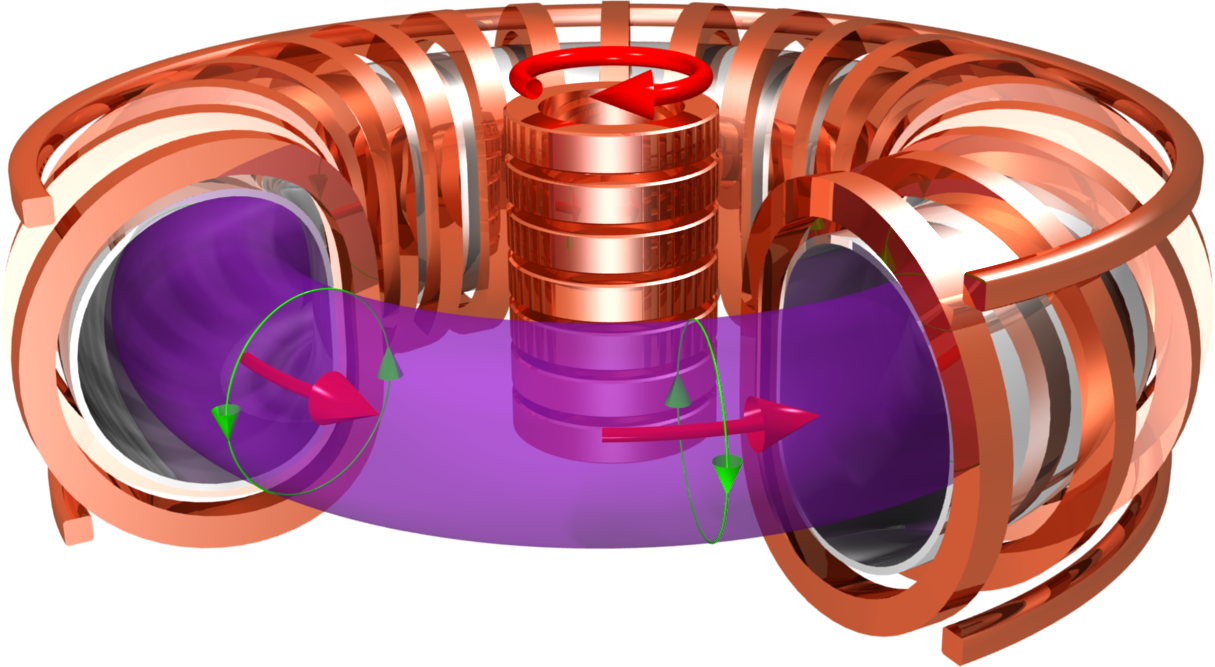
\includegraphics[width=\textwidth]{graphics/7_Tokamak3D_41}
    \caption{Typical tokamak configuration}
    \end{figure}
  \column{0.57\textwidth}

    \begin{block}{Tokamak configuration}
      \begin{itemize}
        \item Toroidal field coils $\Rightarrow$ $B_{\phi}$
        \item Plasma current $\quad \,\,\Rightarrow$ $B_{\theta}$
        \item Poloidal field coils for shaping
        \item Transformer $\Rightarrow$ pulsed operation
      \end{itemize}
    \end{block}
  \end{columns}


\blfootnote{Image: MPI f\"{u}r Plasmaphysik (IPP), accessed from \url{http://www.ideen2020.de/en/51/energy/}}

\end{frame}

%----------------------------------------------------------------------------------------------------%
%----------------------------------------------------------------------------------------------------%

\begin{frame}{Core characteristics for two tokamaks}
\begin{table}\centering
\begin{tabular}{@{}llclcl@{}}\toprule[2 pt]
&\multicolumn{1}{c}{C-Mod} & \phantom{abc} & \multicolumn{1}{c}{DIII-D}  \\
\midrule
\phantom{a}Parameters & &&  \\
\phantom{a}Major radius $R$ [m] 	&	$0.61 - 0.74$	&&	$1.49-1.88$		  	\\
\phantom{a}Minor radius $a$ [m] 	&	$0.169-0.264$	&& 	$0.331-0.752$	          	\\
\phantom{a}Aspect ratio	$R/a$           &       $2.8-3.6$	&&	$2.5-4.5$        	  	\\
\phantom{a}Magnetic field $B$ [T]       &       $2.0-8.0$	&&	$0.5-2.2$                       \\
\phantom{a}Max plasma volume [$\text{m}^3$]	&	1	&&	24			  	\\
\phantom{a}Max  $T_i, T_e$ [keV]	&	5.6, 6.0	&&	27.0, 16.0		  	\\
\phantom{a}Max current $I$ [MA]         &	2.05	        &&	3			  	\\
\phantom{a}Max power density [MW/$\text{m}^3$]	& 6.7    	&&	1.3			  	\\
\phantom{a}Shot length [s] at $B_{max}$  &	1	        &&	6			  	\\
\phantom{a}PFCs	                        &	Mo, W	        &&	C			  	\\
\bottomrule[2 pt]
\end{tabular}
\label{tbl:tokamak_params_juxtaposition}
\end{table}

\tiny{Reproduced from MIT PSFC}

\end{frame}

%----------------------------------------------------------------------------------------------------%
%----------------------------------------------------------------------------------------------------%

\begin{frame}{Core characteristics for two additional tokamaks}
\begin{table}\centering
\begin{tabular}{@{}llclcl@{}}\toprule[2 pt]
& \multicolumn{1}{c}{NSTX}  && \multicolumn{1}{c}{ITER} \\
\midrule
\phantom{a}Parameters & &&  \\
\phantom{a}Major radius $R$ [m] 	&	$0.8-1.0$	 && 	$6.2$		\\
\phantom{a}Minor radius $a$ [m] 	&	$0.5-0.787$	 &&     $2$	        \\
\phantom{a}Aspect ratio	$R/a$           &       $1.27-1.6$	 && 	$3.1$		\\
\phantom{a}Magnetic field $B$ [T]       &  	$0.8 \sim 1.6$	 && 	$3.1$		\\
\phantom{a}Max plasma volume [$\text{m}^3$]	&14        	 && 	700		\\
\phantom{a}Max  $T_i, T_e$ [keV]	&	2.5, 4.1	 && 	30, 30		\\
\phantom{a}Max current $I$ [MA]         &	1.5        	 && 	15		\\
\phantom{a}Max power density [MW/$\text{m}^3$] &	1.1	         && 	0.7		\\
\phantom{a}Shot length [s] at $B_{max}$  &	1.5        	 && 	400		\\
\phantom{a}PFCs	                        &	CFC/Graphite	 && 	W, C and Be	\\
	                                &	Li coating	 && 			\\
\bottomrule[2 pt]
\end{tabular}
\label{tbl:tokamak_params_juxtaposition}
\end{table}

\tiny{Reproduced from MIT PSFC}

\end{frame}

%----------------------------------------------------------------------------------------------------%
%----------------------------------------------------------------------------------------------------%

\begin{frame}{Plasma confinement configurations: stellarators}
  Confinement requires toroidal magnetic fields with a poloidal twist
  \begin{columns}
  \column{0.6\textwidth}
  \begin{block}{Stellarator configuration}
      \begin{itemize}
        \item modular coils $\Rightarrow$ helical field lines
        \item no net plasma current required
        \item steady state operation
      \end{itemize}
    \end{block}
   \column{0.4\textwidth}
    \begin{figure}
    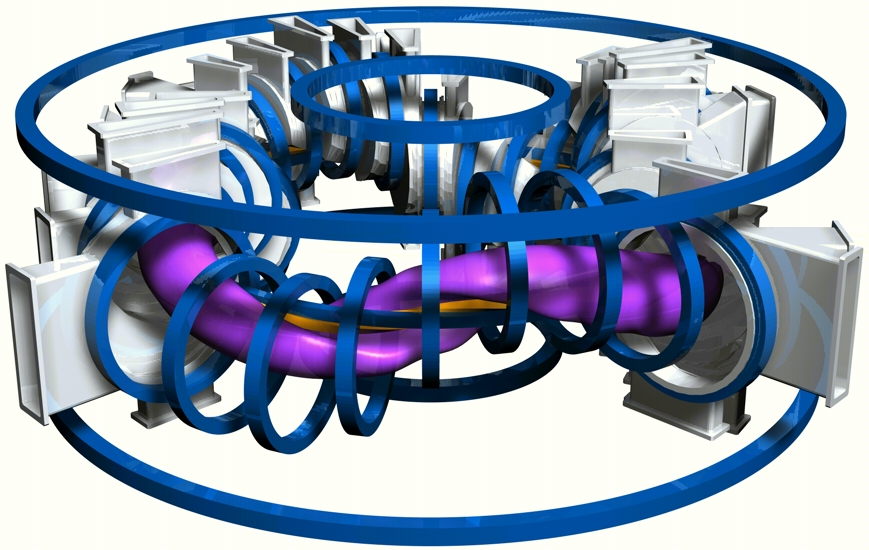
\includegraphics[width=\textwidth]{graphics/TJII_model1}
    \caption{TJII} % http://www-fusion.ciemat.es/New_fusion/en/TJII/presentacion.shtml
    \end{figure}
   \end{columns}
\blfootnote{Image: Laboratorio Nacional de Fusi\'{o}n, CIEMAT, Madrid. \url{http://www-fusion.ciemat.es/New_fusion/en/TJII/presentacion.shtml}}
\end{frame}

%----------------------------------------------------------------------------------------------------%
%----------------------------------------------------------------------------------------------------%

\begin{frame}{Core characteristics for two stellarators}
\begin{table}\centering
\begin{tabular}{@{}llclcl@{}}\toprule[2 pt]
&\multicolumn{1}{c}{HSX} & \phantom{abc} & \multicolumn{1}{c}{LHD}  \\
\midrule
\phantom{a}Parameters & &&  \\
\phantom{a}Major radius $R$ [m] 	&	$1.20$ (avg.)  	&&	$4.0$ (avg.)		  	\\
\phantom{a}Minor radius $a$ [m] 	&	$0.15$ (avg.)	&& 	$0.6$ (avg.)	          	\\
\phantom{a}Aspect ratio	$R/a$           &       $8$      	&&	$6.5$        	  	\\
\phantom{a}Magnetic field $B$ [T]       &       $1.25$	        &&	$3$                       \\
\phantom{a}No. of field periods/$2\pi R_0$ &    4	        &&	5                       \\
\phantom{a}Plasma volume [$\text{m}^3$]	&	0.44     	&&	30			  	\\
\phantom{a}Max  $T_e$ [keV]	        &	$\sim 20 - 25$	&&	$10$		  	\\
\phantom{a}Max power density [MW/$\text{m}^3$]   	&       0.46  	&&	0.040 		  	\\
\phantom{a}Shot length [s] at $B_{max}$  &	1.5        	 && 	127		\\
\bottomrule[2 pt]
\end{tabular}
\label{tbl:tokamak_params_juxtaposition}
\end{table}

\tiny{Data compiled from \url{http://www.hsx.wisc.edu/parameters.shtml}, \url{http://www.lhd.nifs.ac.jp/en/home/lhd.html}, Fujiwara, M. et al. \emph{Plasma confinement studies in LHD}. IAEA-F1-CN-69/EX2/3, and \url{http://www.nifs.ac.jp/itc/itc12/Motojima.pdf}}

\end{frame}

%----------------------------------------------------------------------------------------------------%
%----------------------------------------------------------------------------------------------------%

\begin{frame}{The focus of this work is to simulate the edge}
\begin{figure}[h!]
  \centering
    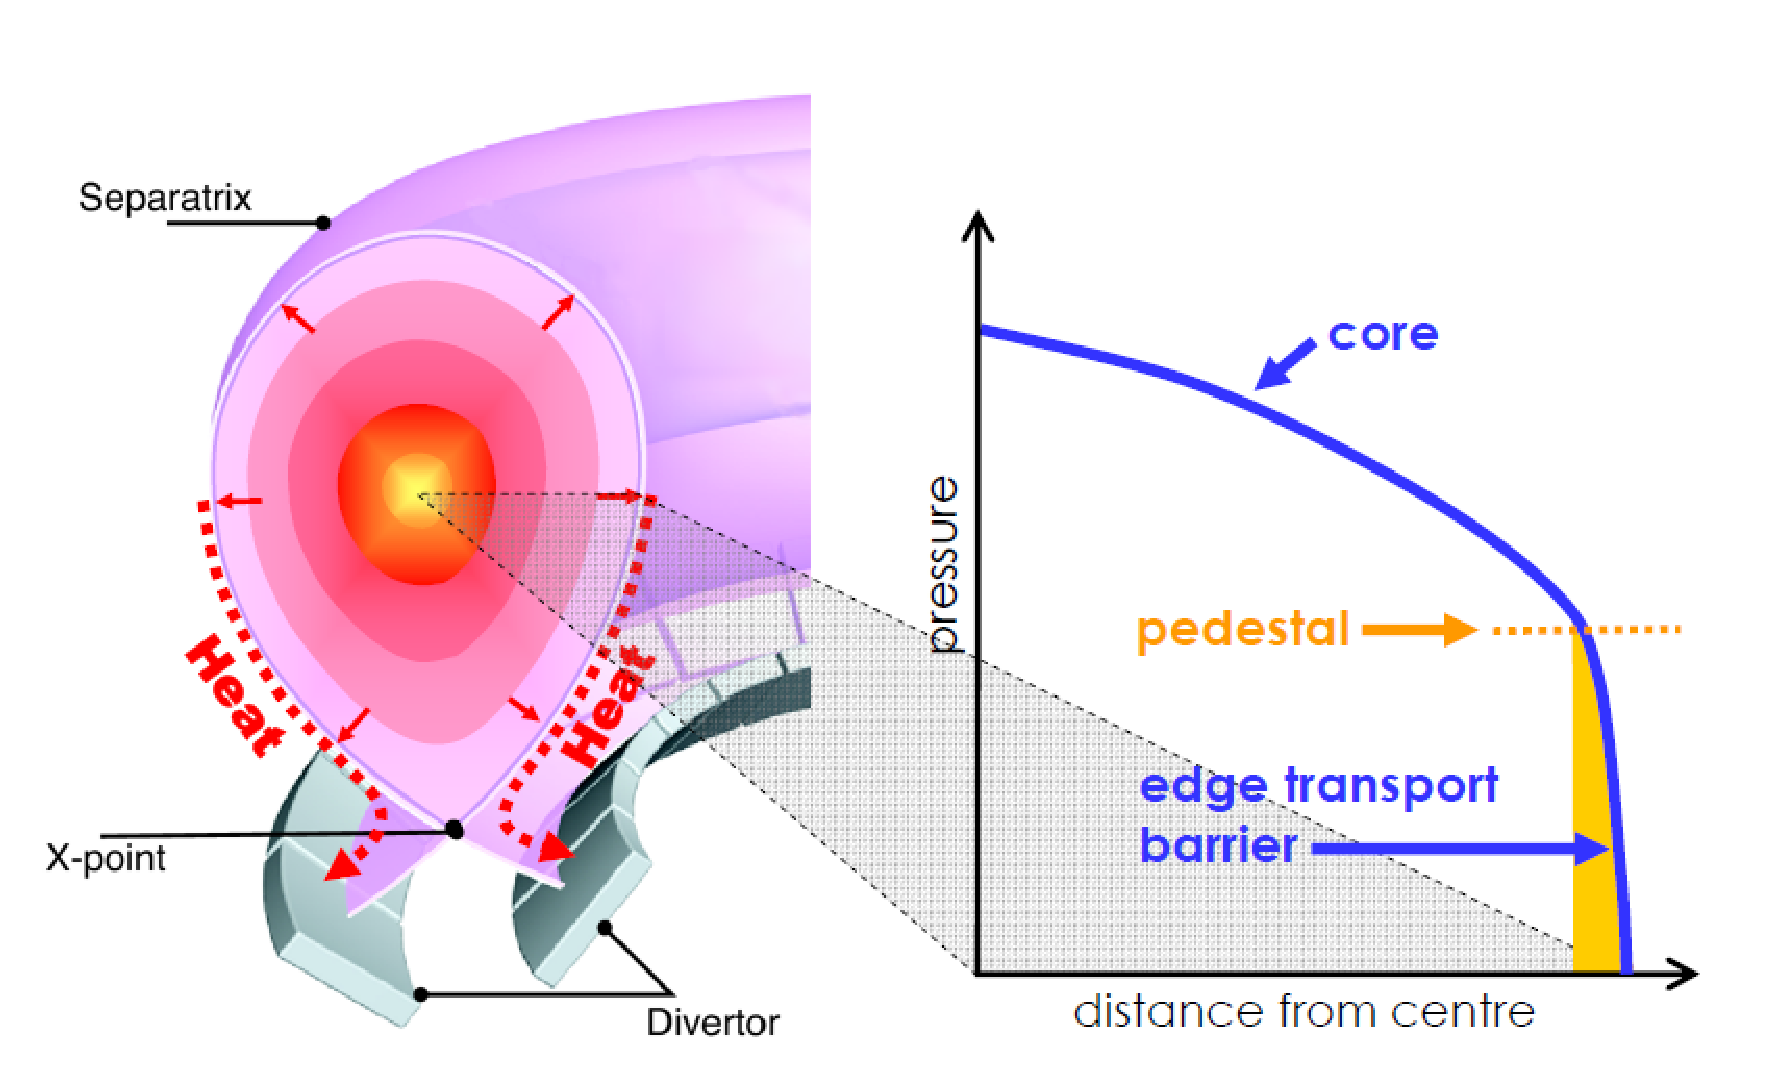
\includegraphics[width=0.75\textwidth]{graphics/pedestal_and_poloidal_xsec}
  \caption{A poloidal cross-section of the magnetic configuration is shown on the left, whereas the plasma pressure from the core center to the edge is shown for the indicated radial arm\blfootnote{Connor, J.W., et al. Edge localised modes (ELMs): experiments and theory. Presented at the first ITER international summer school.}}
\end{figure}
\end{frame}

%----------------------------------------------------------------------------------------------------%
%----------------------------------------------------------------------------------------------------%

\begin{frame}{The edge defines a region of vastly different scales}
\begin{columns}
  \column{0.5\textwidth}
    \begin{figure}
    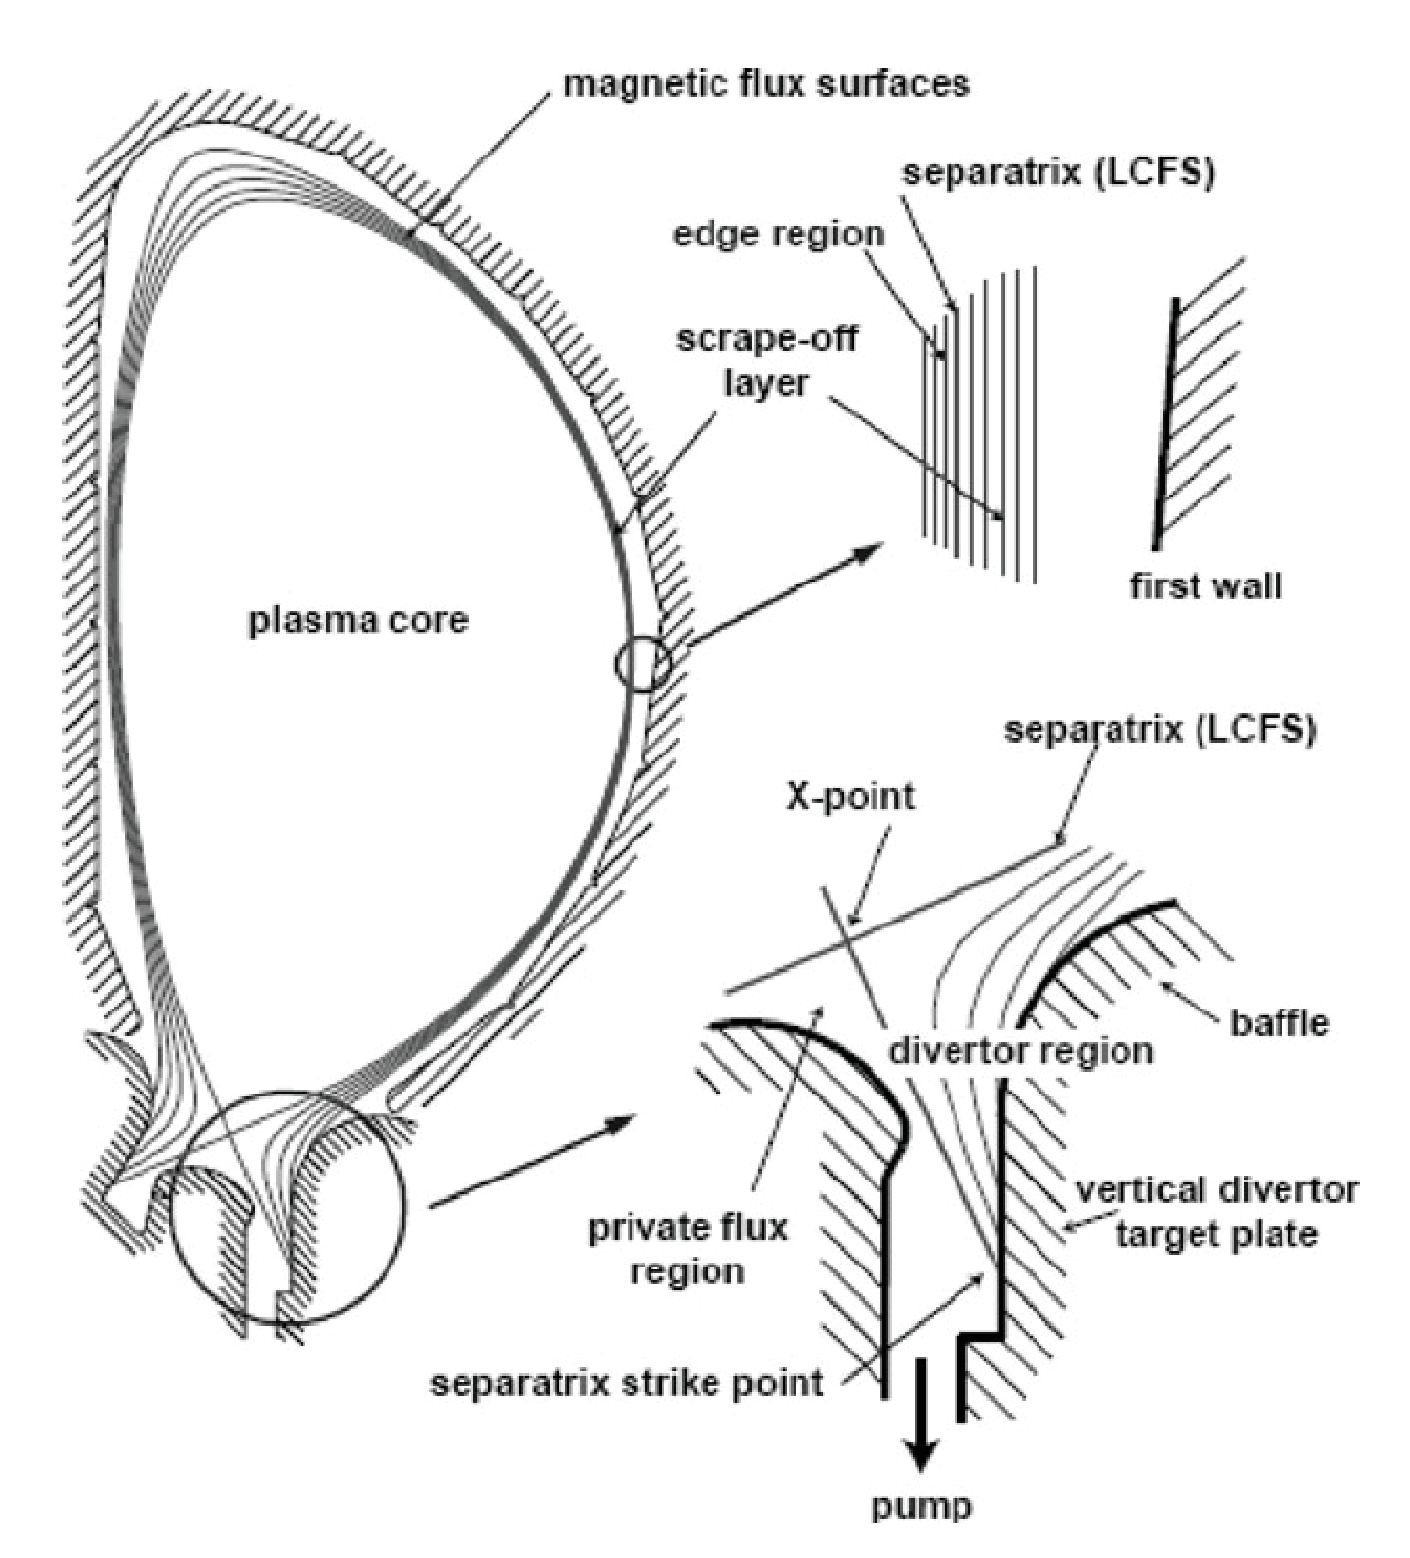
\includegraphics[height=6cm, keepaspectratio]{graphics/edge_anatomy}
    \end{figure}
  \column{0.5\textwidth}
core radius: $\sim$ $10^{-1} - 10^0$ m \\
edge thickness: $\sim$ $10^{-3} - 10^{-2}$ m
    \begin{block}{Edge features}
      \begin{itemize}
        \item last closed flux surface (LCFS): \emph{separatrix}
        \item region outboard of LCFS: \emph{scrape-off layer} (SOL)
        \item material boundaries (PFCs)
        \item \emph{not} generally at LTE
        \item \emph{not} guaranteed to be collisional (cf. next slide)
      \end{itemize}
    \end{block}
  \end{columns}

\blfootnote{Image: Stangeby, P.C. \emph{The Plasma Boundary of Magnetic Fusion Devices}. CRC Publishing, Bristol, England, United Kingdom, January 2000.}

\end{frame}

%----------------------------------------------------------------------------------------------------%
%----------------------------------------------------------------------------------------------------%

\begin{frame}{Edge region exhibits variability}
\begin{table}\centering
%\ra{1.4}
\begin{tabular}{@{}llclclcl@{}}\toprule[2 pt]
&\multicolumn{1}{c}{JET} & \phantom{abc} & \multicolumn{1}{c}{C-mod} \\
\midrule
\phantom{a}Parameters & &&  \\
\phantom{a}electron density $n_e$ [$\text{m}^{-3}$]	&	$10^{19}$	&&	$10^{20} -10^{21}$       \\
\phantom{a}$T_e$ [eV]	&	50	&&	10 \\
\phantom{a}Connection length $L$ [m]         &	40	        &&	8	\\
\phantom{a}$\nu_e^* = \nu_e / \nu_{e,bounce}$	& 25    	&&	1000	\\
\phantom{a}self-collisional mean free paths $\lambda_{ee}, \lambda_{ii}$ [m]  &	2.5	        &&	0.01	\\
\phantom{a}SOL dwell time $\tau_{SOL} = L / c_s$ [ms]  &	0.6	        &&	0.3	\\
\bottomrule[2 pt]
\end{tabular}
\caption{Parameters in the scrape-off layer (SOL) for two tokamak devices.}
\end{table}

\blfootnote{Table: Stangeby, P.C. \emph{The Plasma Boundary of Magnetic Fusion Devices}. CRC Publishing, Bristol, England, United Kingdom, January 2000.}

\end{frame}

%----------------------------------------------------------------------------------------------------%
%----------------------------------------------------------------------------------------------------%

\begin{frame}{Edge physics affects core confinement}
\begin{itemize}
\item Edge conditions determine to a great extent the quality of confinement and dictate transport in the \emph{core}.

\begin{figure}
  \centering
    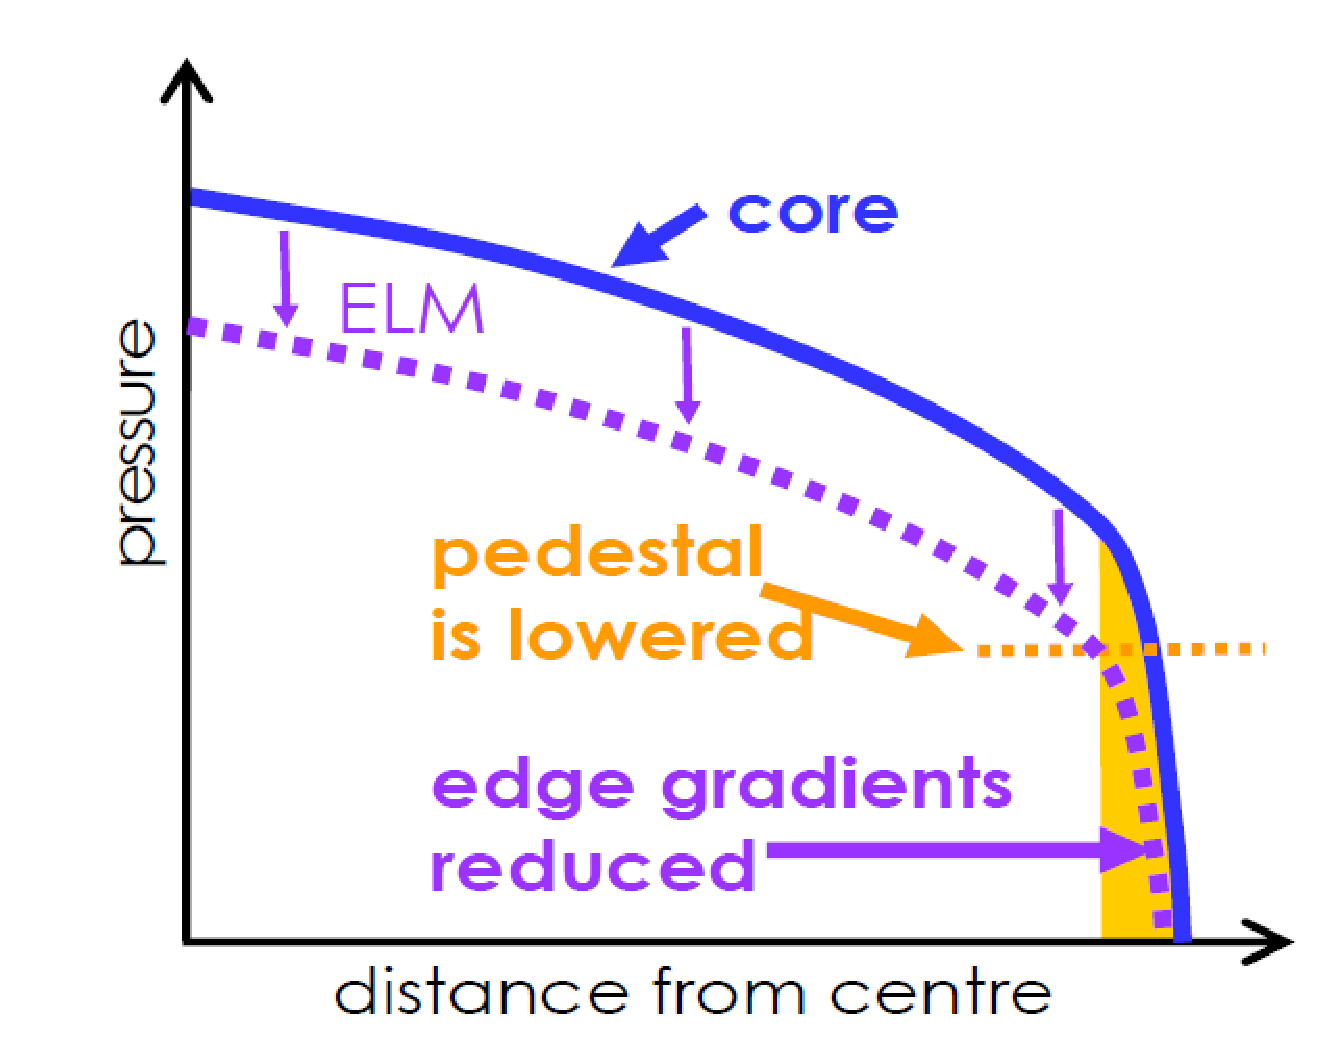
\includegraphics[width=0.45\textwidth]{graphics/ELM_effect_on_confinement}
  \caption{When any means (e.g. ELMs) causes removal of density from the edge region, the edge gradients decrease and so does the pedestal which directly reduces the confinement of the core.}
%  \label{fig:ELM_effecT_on_confinement}
\end{figure}
\end{itemize}

\blfootnote{Connor, J.W., et al. Edge localised modes (ELMs): experiments and theory. Presented at the first ITER international summer school.}

\end{frame}

%----------------------------------------------------------------------------------------------------%
%----------------------------------------------------------------------------------------------------%

\begin{frame}{The edge defines a region of vastly different scales}
  \begin{columns}
  \column{0.5\textwidth}
    \begin{figure}
    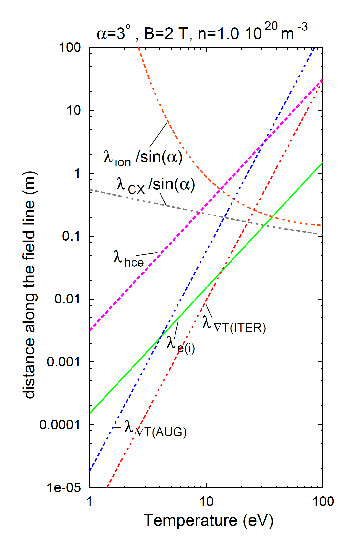
\includegraphics[width=\textwidth, height = 6.5cm, keepaspectratio]{graphics/lengthscales_SOL}
%    \caption{SOL length scales for magnetic field line angle of incidence of $3^{\circ}$ with respect to the surface normal [Schneider] } %
    \end{figure}
     \column{0.5\textwidth}
    \begin{figure}
    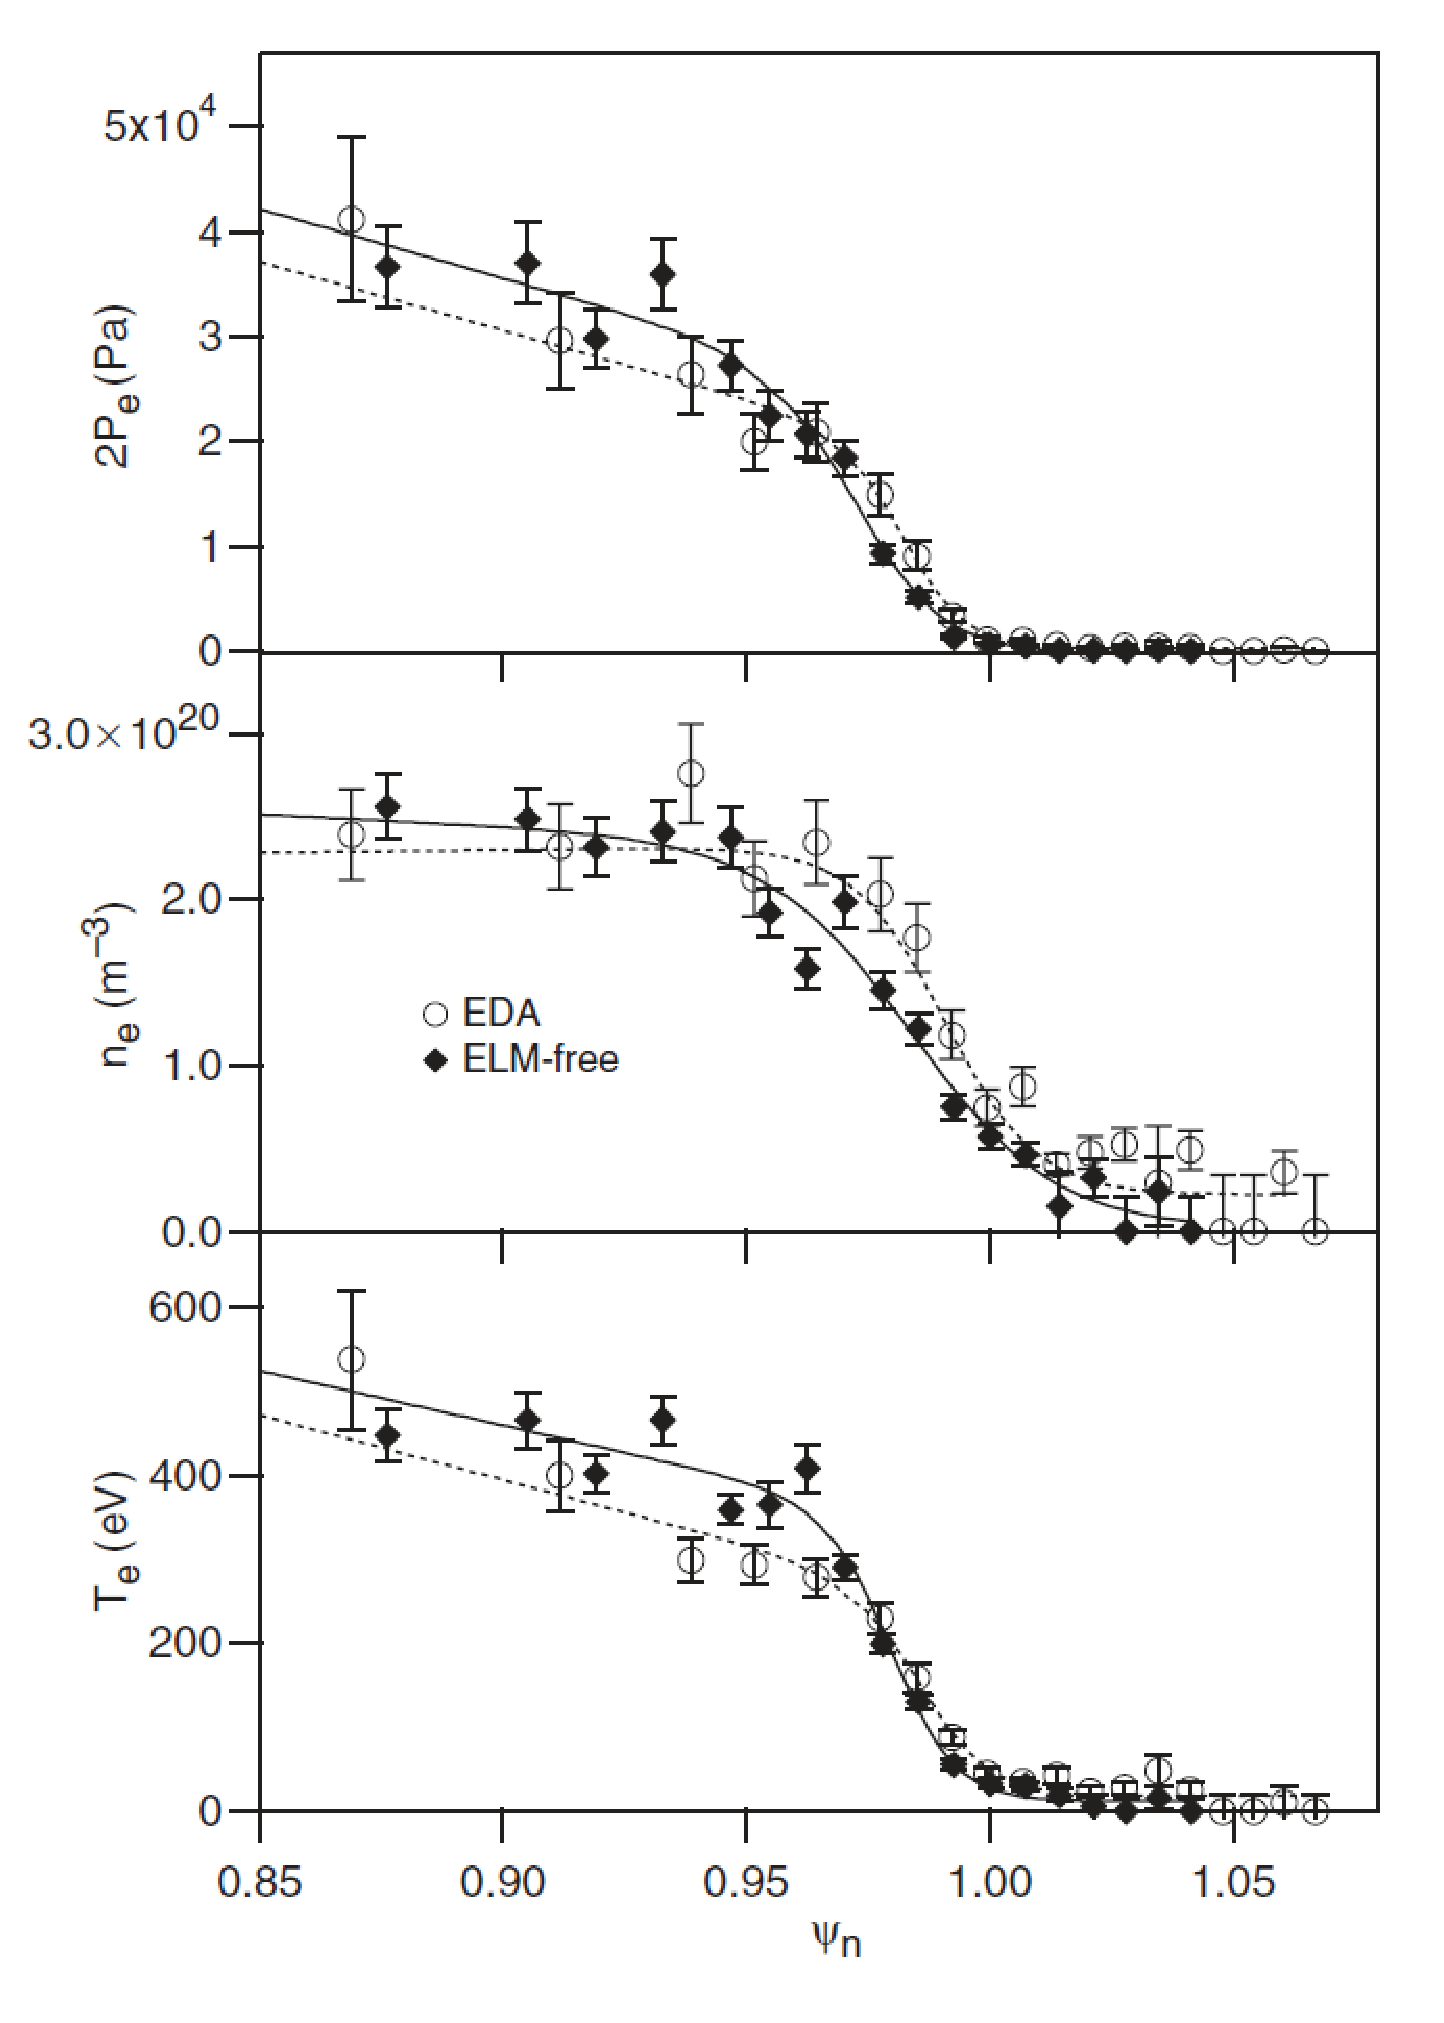
\includegraphics[height = 6.5cm, keepaspectratio]{graphics/pedestal_traces}
 %   \caption{SOL parameters, p.21 Stangeby } %
    \end{figure}
   \end{columns}

\blfootnote{Left image: Stangeby, P.C. \emph{The Plasma Boundary of Magnetic Fusion Devices}. CRC Publishing, Bristol, England, United Kingdom, January 2000., Right image: Mossessian, D. A. et al. \emph{H-mode pedestal characteristics and MHD stability of the edge plasma in Alcator C-mod.} Plasma physics and controlled fusion 44, 4 (2002), 423}

  \end{frame}

%----------------------------------------------------------------------------------------------------%
%----------------------------------------------------------------------------------------------------%

\begin{frame}{The utility of computer simulation}
\begin{center} \fbox{Theory} $\Leftrightarrow$ \fbox{Computation} $\Leftrightarrow$ \fbox{Experiment}\end{center}
Computer simulations are indispensible in contributing to the understanding of magnetically confined plasmas
\begin{itemize}
\item Numerical simulations help guide experiments by
  \begin{itemize}
    \item simulating and fine-tuning proposed experiments % $\Rightarrow$ reduces burden on experiments, and focuses both efforts and time
    \item producing results that have not yet been explored
    \item post-processing can simulate diagnostic measurements
    \item numerical solutions can aid design of devices (e.g. stellarators)
    \end{itemize}
\item Numerical simulations can access costly ventures (e.g. the \emph{burning plasma} experiment)
\item As more detailed and higher fidelity computational models are developed, the utility of computation increases and the feedback cycle becomes more efficient and useful.
\end{itemize}
\end{frame}

%----------------------------------------------------------------------------------------------------%
%----------------------------------------------------------------------------------------------------%

\begin{frame}{Examples of contributions from computation}
Computation contributes in manifold ways to theory/experiment:
\begin{itemize}
\item \textbf{Global stability and major disruption prevention}: By predicting the particular circumstances that cause them, e.g. Fredickson, et al explained TFTR discharge collapse\footnote{E. Fredrickson, W. Park, et al, “High-beta disruption in tokamaks”} %, \\Phys. Rev. Lett, 75 1763 (1995)}
\begin{itemize}
\item Most energetically favorable configuration for that discharge caused relaxation to a long wavelength helical structure (nonlinear evolution to 3D equilibrium)
\item The resulting equilibrium aligns with the curvature of the device such that a pressure gradient is present in the bad curvature side
\item The local pressure bulge pushes outboard $\Rightarrow$ stochastization $\Rightarrow$ thermal quench
\end{itemize}
\end{itemize}

\end{frame}

%----------------------------------------------------------------------------------------------------%
%----------------------------------------------------------------------------------------------------%

\begin{frame}{Examples of contributions from computation}
Computation contributes in manifold ways to theory/experiment:
\begin{itemize}
\item \textbf{Design of three dimensional configurations}:
\begin{itemize}
\item Optimized 3D codes in $N$ parameter space (e.g. 30$\sim$40 Fourier modes) can be used to explore magnetic topologies that meet desired transport, stability, and confinement requirements $\Rightarrow$ \textbf{stellarators}\footnote{A. S. Ware et al., “High-beta equilibria of drift-optimized compact stellarators”, Phys.Rev. Lett. 89, 125503 (2002)}
\item Examples: Quasi-poloidal compact stellarator (QPS) at ORNL, NCSX at PPPL\footnote{Fusion simulation project (FSP): integrated simulation \& optimization of fusion systems. December 1, 2002.}
\end{itemize}
\end{itemize}


\end{frame}

%----------------------------------------------------------------------------------------------------%
%----------------------------------------------------------------------------------------------------%

\begin{frame}{Examples of contributions from computation}
Computation contributes in manifold ways to theory/experiment:
\begin{itemize}
\item \textbf{Computation has informed theory}:
\begin{itemize}
\item \emph{Experiment}: H-mode is accompanied by abrupt increase in poloidal rotation in pedestal region.
\item \emph{Computation}: Turbulence can spontaneously generate large radial flows $\Rightarrow$ transport barrier, agreement between gyrofluid and gyrokinetic codes!
\item \emph{Theory}: Experiment and numerical confirmations of Reynolds-stress-generated flows put on sound foundation through several analytical studies.
\end{itemize}
\end{itemize}

\blfootnote{A. Hasegawa and M. Wakatani, “Self-organization of electrostatic turbulence in a cylindrical plasma”, Phys.Rev. Lett. 59, 1581 (1987). }

\end{frame}

%----------------------------------------------------------------------------------------------------%

\subsection{Numerical challenges}

%----------------------------------------------------------------------------------------------------%
%----------------------------------------------------------------------------------------------------%
\begin{frame}{Numerical challenges}
\begin{enumerate}
\item \textbf{Multiple species}: electrons, multiple ions, neutrals\\[0.5em]
\item \textbf{Time scales} span  $9 - 12$ orders of magnitude
\begin{itemize}
\item $\Omega_{ce}^{-1} \gtrsim 10^{-10}$ s : RF heating time scale \\[0.5em]
\item $\tau\phantom{_{ce}^{-1}} \lesssim 10^{2}\phantom{^{-0}}$ \,s : discharge time scale
\end{itemize}
\item \textbf{Spatial scales} span $4 - 6$ orders of magnitude
\begin{itemize}
\item $\lambda_{e,\nabla T} \gtrsim 10^{-5}$ m : $\nabla T$ length scale for electron conduction \\[0.5em]
\item $L\phantom{_{e,\nabla T}} \lesssim 40\phantom{^{-5}}$ m : connection length
\end{itemize}
\item \textbf{Velocity scales} span $\sim 7$ orders of magnitude
\begin{itemize}
\item $v_n\phantom{_i} \quad \,\,\,\,\sim 0$ \qquad \,\,\,\,\,\,\,\,\,\, re-emitted neutrals adsorbed on wall \\[0.5em]
\item $v_{Ti} \quad \,\,\,\,\sim 36.12$ \quad \,\,\,\, m/s for $H^+$ thermal ions $T_i = 0.025$ eV\\[0.5em]
\item $v_{Te,SOL} \sim 10^6$\qquad\,\,\,\,\,\,\,m/s for $e^-$ in edge $T_e = 10 - 50$ eV \\ [0.5em]  
\item $v_{Te} \quad \,\,\,\sim 7.26\times 10^{7}$ m/s for $e^-$ at max $T_e \sim 30$ keV \\[0.5em]
\end{itemize}
\end{enumerate}

Fully dimensional simulation requires $10^{11}$ phase space cells with $10^8$ time steps over full discharge based on physical scales alone

 

\end{frame}

%----------------------------------------------------------------------------------------------------%
%----------------------------------------------------------------------------------------------------%

\begin{frame}{The vastness in scales has motivated isolated codes}
   \centering
    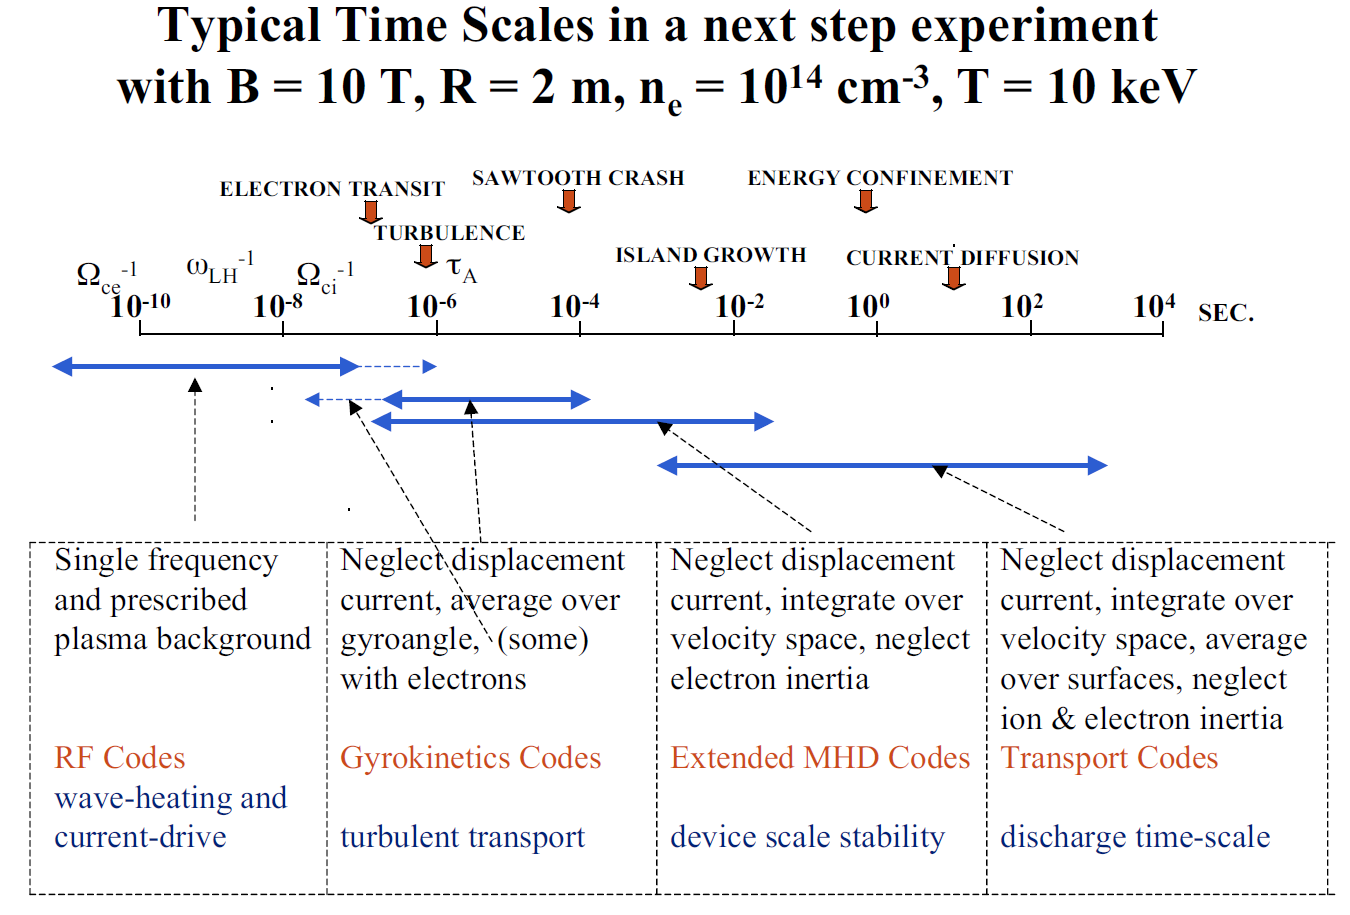
\includegraphics[width=0.912\textwidth]{graphics/codes_timescales}


\blfootnote{FESAC ISOFS subcommittee. \emph{Fusion simulation project (FSP): integrated simulation \& optimization of fusion systems}. December 1, 2002.}

\end{frame}

%----------------------------------------------------------------------------------------------------%
%----------------------------------------------------------------------------------------------------%

\begin{frame}{Numerical challenges, cont'd}
\begin{enumerate}  
\item \textbf{Multiple collisional processes}\footnote{G\"{u}\c{c}lu, Y., et al. \emph{Arbitrarily high-order semi-Lagrangian methods for the kinetic description of plasmas}, October 2, 2013}:\\[0.5em]
\begin{itemize}
\item \underline{\emph{elastic}}: Coulomb (charged particles), Van der Waals (neutrals), charged particle - neutral momentum exchange\\[0.3em]
\item \underline{\emph{inelastic}}: excitation, ionization, recombination, attachment, dissociation, etc. \\[0.3em]
\item collision operator requires integral formulation in most cases\\[0.3em]
\end{itemize} 
\item \textbf{Other challenges}: \\[0.5em]

\begin{itemize}
\item long-range nature of EM forces $\Rightarrow$ ``grazing collisions''\\[0.3em]
\item radiation transport $\Rightarrow$ need opacity and emissivity feedback \\[0.3em]
\item plasma-surface interaction \\[0.3em]
\item if non-LTE, require atomic rate kinetics  \\[0.3em]
\end{itemize}
\end{enumerate}
\end{frame}

%----------------------------------------------------------------------------------------------------%
%----------------------------------------------------------------------------------------------------%

\begin{frame}{The need for deterministic semi-Lagrangian solutions}
Deterministic solutions offer clear advantages:
\begin{itemize}
\item Statistical methods must simulate enough particles to resolve sparse regions $\Rightarrow$ high computational cost
\item Deterministic models can:
\begin{itemize}
\item resolve high energy tail $\Rightarrow$ accurate ionization rates
\item resolve electric fields in quasi-neutral regions; require no partitioning of scales
\end{itemize}
\end{itemize}

Alternative numerical solutions have disadvantages:

\begin{itemize}
\item \textbf{\emph{Eulerian}} : strict time step requirement (CFL number), significant memory storage for a needed high resolution mesh
\item \textbf{\emph{Lagrangian}} : no CFL restriction, but require a Green's function to propagate solution. 
\item \textbf{\emph{Semi-Lagrangian}} : no CFL restriction, trajectories pushed along known characteristic curves
\end{itemize}



\end{frame}

%----------------------------------------------------------------------------------------------------%
%----------------------------------------------------------------------------------------------------%


%\item Sparse regions of phase space require statistical solutions to simulate large number of particles to sufficienlty resolve
%\item  $\Rightarrow$ Deterministic solutions have significant advantage

%----------------------------------------------------------------------------------------------------%
%----------------------------------------------------------------------------------------------------%

%----------------------------------------------------------------------------------------------------%
%----------------------------------------------------------------------------------------------------%

\subsection{Model equations}

%----------------------------------------------------------------------------------------------------%
%----------------------------------------------------------------------------------------------------%

\begin{frame}{\subsecname} % model equations 
The plasma system is described by distribution functions for each particle species $\alpha$:
$$f_{\alpha} = f_{\alpha}(t,\vec{x},\vec{v}) \, : \, \mathbb{R}^+ \times \mathbb{R}^{d_x} \times \mathbb{R}^{d_v} \mapsto \mathbb{R}$$

the evolution of which is tied to the Boltzmann-Maxwell system:

\begin{equation*}
\frac{\partial f_{\alpha}}{\partial t} + \vec{v}\cdot \frac{\partial f_{\alpha}}{\partial \vec{x}} + \frac{q_{\alpha}}{m_{\alpha}}\left( \vec{E} + \vec{v} \times \vec{B}\right)\cdot \frac{\partial f_{\alpha}}{\partial \vec{v}}  =  \left(\frac{\partial f_{\alpha}}{\partial t}\right)_{coll}\end{equation*}\\[0.9em]
\vspace{-1em}
\begin{eqnarray*}
\epsilon_0\vec{\nabla}\cdot \vec{E} =\sum_{\alpha} q_{\alpha}\int f_{\alpha}(t,\vec{x},\vec{v}) d^3\vec{v} \,\, &,& \vec{\nabla}\cdot\vec{B} = 0\\
\vec{\nabla} \times \vec{B} = \mu_0\sum_{\alpha} q_{\alpha} \int \vec{v}\,f_{\alpha}(t,\vec{x},\vec{v}) d^3\vec{v} + \frac{1}{c^2}\frac{\partial\vec{E}}{\partial t} &,& \vec{\nabla}\times\vec{E} = -\frac{\partial\vec{B}}{\partial t} \label{eq:Maxwell34}
\end{eqnarray*} 

\end{frame}

%----------------------------------------------------------------------------------------------------%


%\begin{frame}{movie test slide}
%Variable velocity field $v(x)$  \\
%\movie[autostart,loop]{}{movies/N_v_S_F8_Nx256Nt400.mpeg}
%\end{frame}

\section{Literature review}

\subsection{Alternative approaches}



%----------------------------------------------------------------------------------------------------%
%----------------------------------------------------------------------------------------------------%

\begin{frame}{Eulerian schemes}
$$\frac{\partial f_{\alpha}}{\partial t} + \vec{v}\cdot \frac{\partial f_{\alpha}}{\partial \vec{x}} + \frac{q_{\alpha}}{m_{\alpha}}\left( \vec{E} + \vec{v} \times \vec{B}\right)\cdot \frac{\partial f_{\alpha}}{\partial \vec{v}}  =  \left(\frac{\partial f_{\alpha}}{\partial t}\right)_{coll}$$

\begin{itemize}
\item Distribution function $f_{\alpha} = f_{\alpha}(t,\vec{x},\vec{v})$ lies on a fixed grid
\item $(t,\vec{x},\vec{v})$ are independent variables
\item Derivatives are replaced with $N$th order finite differences
\item Severe time step restriction (Courant-Friedrichs-Lewy, CFL) parameter to ensure stability

$$\text{e.g. } \qquad |\mathcal{C}| \coloneqq |\tfrac{v\Delta t}{\Delta x}| \leq \delta, \delta \in\mathbb{R}$$

\item usually requires the fine meshes with many phase space cells $\Rightarrow$ large memory requirements and costly numerical solutions

\item Examples: WENO, MUSCL

\end{itemize}

\end{frame}

%----------------------------------------------------------------------------------------------------%
%----------------------------------------------------------------------------------------------------%

\begin{frame}{Lagrangian schemes}

The distribution $f_{\alpha} = f_{\alpha}(t,\vec{x}(t),\vec{v}(t))$ is evolved in a moving frame:
 
$$\frac{df_{\alpha}}{dt} =  \left(\frac{\partial f_{\alpha}}{\partial t}\right)_{coll}$$

defined by characteristics corresponding to particle trajectories:

$$\frac{d\vec{x}}{dt} = \vec{v}, \qquad \text{and } \qquad \frac{d\vec{v}}{dt} =  \frac{q_{\alpha}}{m_{\alpha}}\left( \vec{E} + \vec{v} \times \vec{B}\right)$$

Solution is obtained by computing
$$f_{\alpha}(t,\vec{x},\vec{v}) = \int d\vec{x}' d\vec{v}' G(t,\vec{x},\vec{v}; t',\vec{x}',\vec{v}') f_{\alpha}(t',\vec{x}',\vec{v}'), \quad t > t'$$

$\Rightarrow$ need Green's function for particular problem\footnote{Wichaidit, and Hitchon, W.N.G. \emph{Propagator methods for plasma simulations: application ot breakdown}. J. Comput. Phys. \textbf{203} (2005) p.650--667}

\end{frame}
 
%----------------------------------------------------------------------------------------------------%
%----------------------------------------------------------------------------------------------------%


\subsection{Semi-Lagrangian methods}

%----------------------------------------------------------------------------------------------------%
%----------------------------------------------------------------------------------------------------%

\begin{frame}{\subsecname}
The distribution $f_{\alpha} = f_{\alpha}(t,\vec{x},\vec{v})$ lies on a fixed grid. Two steps:

\begin{enumerate}
\item \emph{\underline{Eulerian step}}: Update velocities according to collisions on fixed grid:
$$\frac{\partial f_{\alpha}}{\partial t} = \left(\frac{\partial f_{\alpha}}{\partial t}\right)_{coll}$$ 
\item \emph{\underline{Lagrangian step}}: Solve collisionless equation on Lagrangian mesh:
$$\frac{df_{\alpha}}{dt} = 0$$
by convecting $f_{\alpha}(t,\vec{x},\vec{v})$ along characteristics over a step $\Delta t$
$$\frac{d\vec{x}}{dt} = \vec{v}, \qquad \text{and } \qquad \frac{d\vec{v}}{dt} =  \frac{q_{\alpha}}{m_{\alpha}}\left( \vec{E} + \vec{v} \times \vec{B}\right)$$

Remap $f_{\alpha}(t + \Delta t, \vec{x}, \vec{v})$ to Eulerian mesh

\end{enumerate} 

Examples: Cheng and Knorr,  CS, discontinuous Galerkin
  
%\blfootnote{Cheng, C.Z., and Knorr, G. \emph{The integration of the Vlasov equation in configuration space}. J. Comput. Phys. \textbf{22} (1976), p.330--351}
%\blfootnote{G\"{u}\c{c}lu, Y. et al. \emph{A high order cell-centered semi-Lagrangian scheme for multidimensional kinetic simulations of neutral gas flows}. J. Comput. Phys. \textbf{231} (2012)}
%\blfootnote{Rossmanith, J. A. and Seal, D.C. \emph{A positivity-preserving high-order semi-Lagrangian discontinuous Galerkin scheme for the Vlasov-Poisson equations}. J. Comput. Phys. \textbf{230}, 16 (2011), p.6203--6232}

\end{frame}

%----------------------------------------------------------------------------------------------------%
%----------------------------------------------------------------------------------------------------%


\subsection{Classic convected scheme}

%----------------------------------------------------------------------------------------------------%

\begin{frame}{\subsecname}
  
\begin{enumerate}
  \setcounter{enumi}{1}
 
\item \emph{\underline{Lagrangian step}}: convect $f_{\alpha}(t_0,\vec{x}_0,\vec{v}_0) \rightarrow f_{\alpha}(t,\vec{x},\vec{v})$ along characteristics:
$$\frac{d\vec{x}}{dt} = \vec{v}, \qquad \text{and } \qquad \frac{d\vec{v}}{dt} =  \frac{q_{\alpha}}{m_{\alpha}}\left( \vec{E} + \vec{v} \times \vec{B}\right)$$

\textbf{Remap $f_{\alpha}(t, \vec{x}, \vec{v})$ to Eulerian mesh}
\end{enumerate} \vspace{0.4em} 

\begin{columns}
\column{0.5\textwidth}
Moving cell (MC) is a control volume:\\[1em]
  
$\int_{MC(t)} f(t,\vec{x},\vec{v})d^3\vec{x}d^3\vec{v}$ \\[1em]  $= \int_{MC(t_0)} f(t_0,\vec{x}_0,\vec{v}_0)d^3\vec{x}_0d^3\vec{v}_0$
\column{0.5\textwidth}
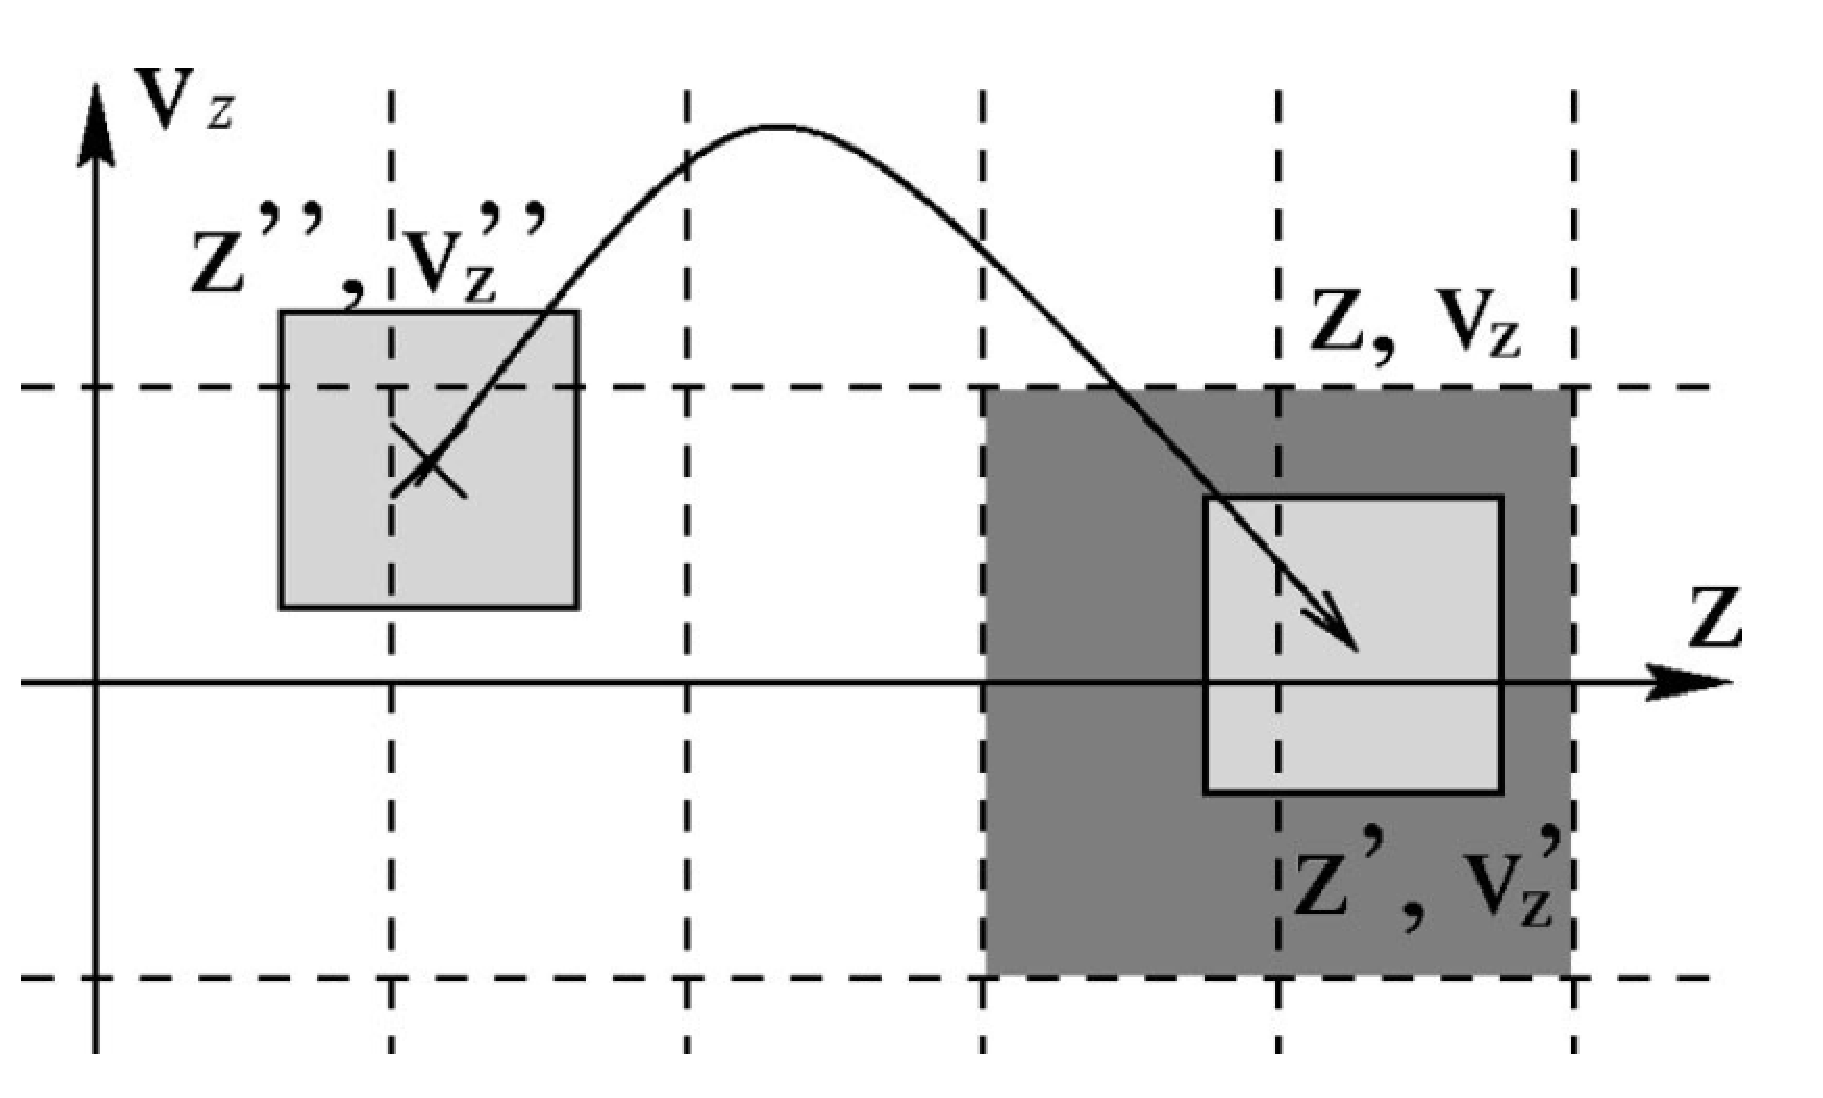
\includegraphics[scale=0.18]{graphics/remap_rule}\\
If $f_{MC}$ is constant $\Rightarrow$ Remap to each cells at $(\vec{x},\vec{v})$ according to cell volume overlap
\end{columns}

%\blfootnote{Image: Feng, J., Hitchon, W.N.G. \emph{Self-consistent kinetic simulations of plasmas}. Physical Review E \textbf{61}, 3 (2000)}

\end{frame}

%----------------------------------------------------------------------------------------------------%

\subsection{High order convected scheme}

%----------------------------------------------------------------------------------------------------%

\begin{frame}{\subsecname : motivation}
\textbf{Problem}: remapping assignment has $\mathcal{O}(\Delta x^2)$ error 
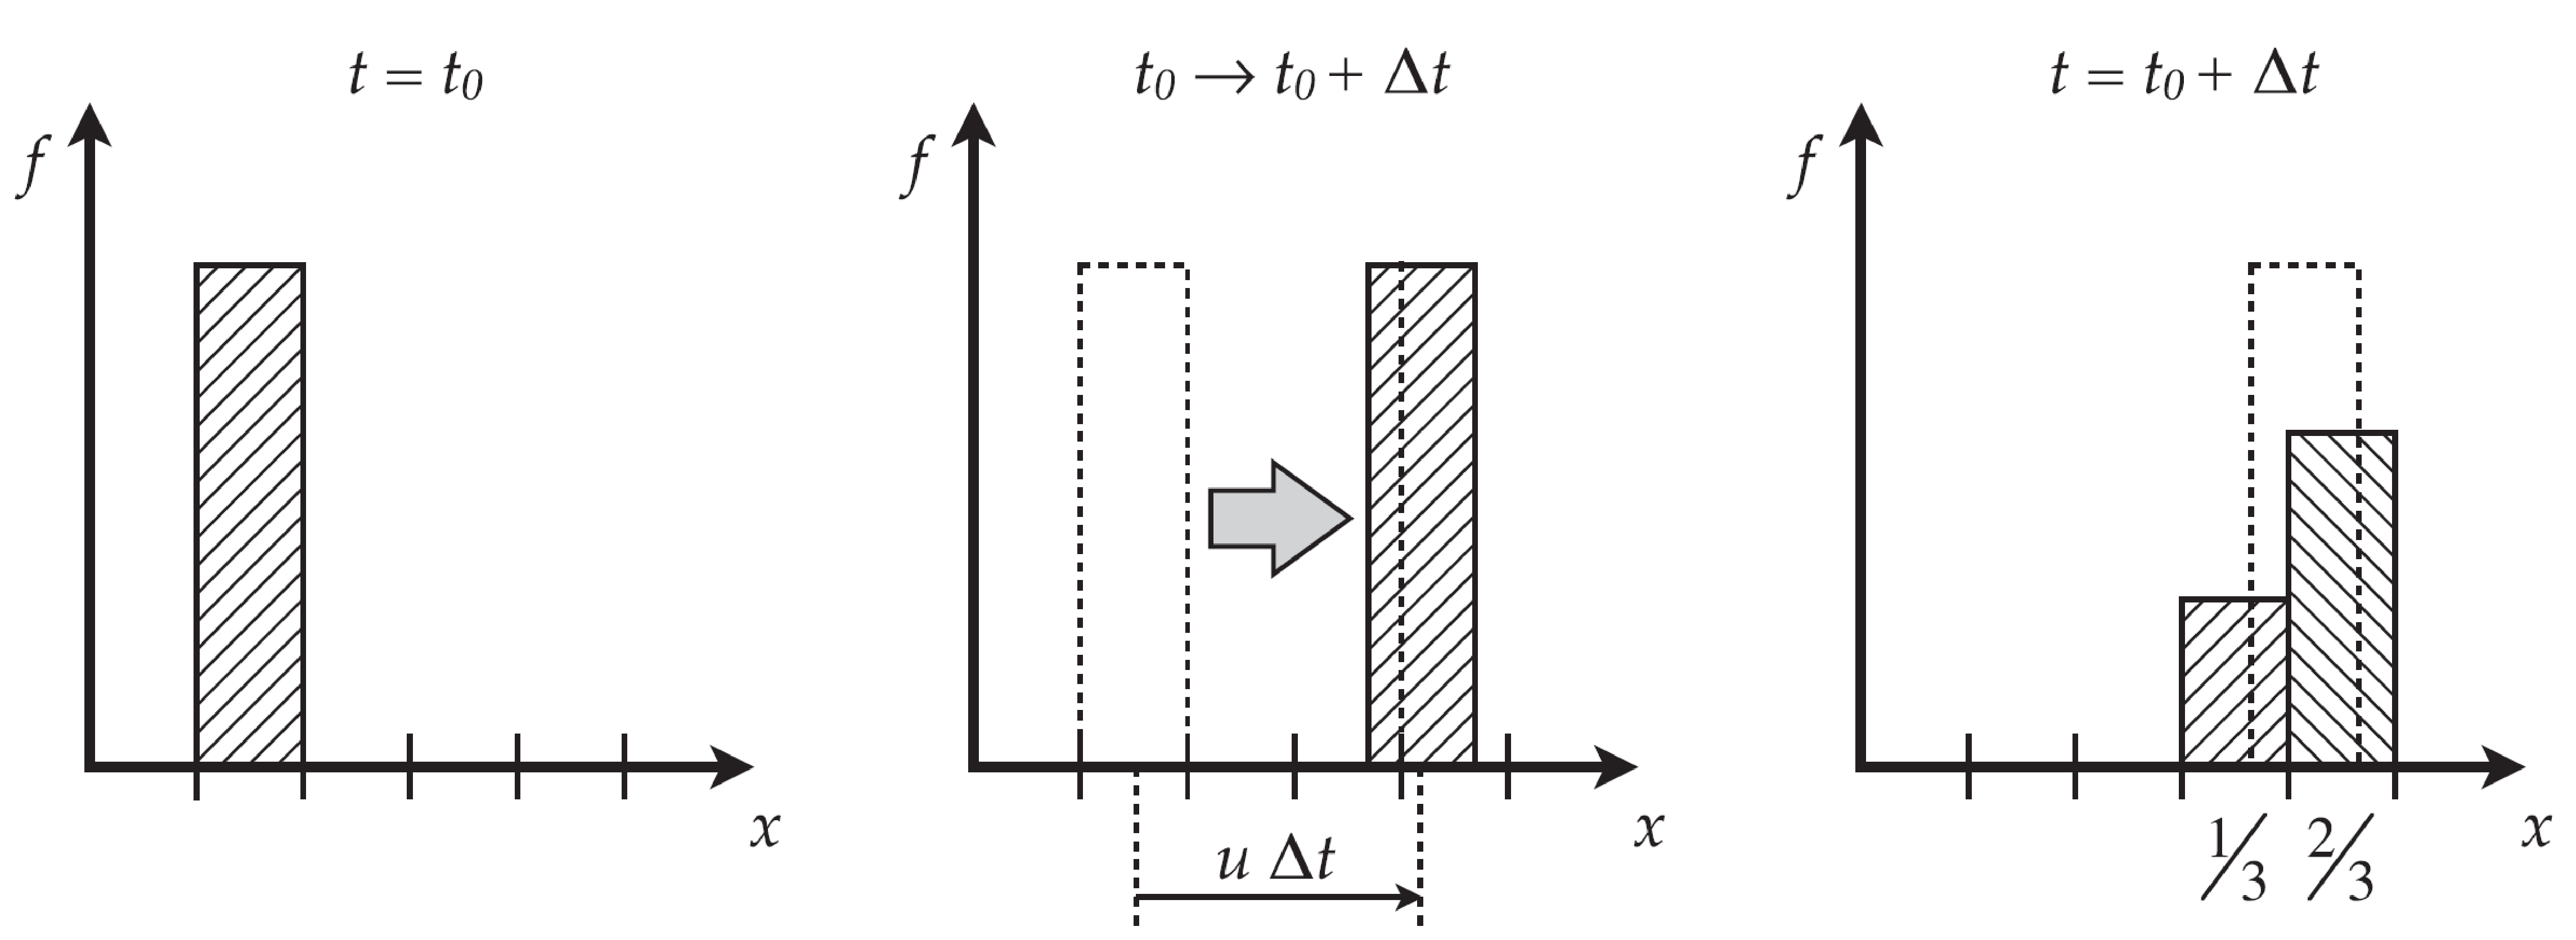
\includegraphics[width=\textwidth]{graphics/ClassicCS_diffusion}

Through modified equation analysis\footnote{Image: G\"{u}\c{c}lu, Y. et al. \emph{A high order cell-centered semi-Lagrangian scheme for multidimensional kinetic simulations of neutral gas flows}. J. Comput. Phys. \textbf{231} (2012)} this error is identified as \underline{\emph{numerical diffusion}}



\end{frame}

%----------------------------------------------------------------------------------------------------%
%----------------------------------------------------------------------------------------------------%

\begin{frame}{Higher order convected scheme}

The 1D constant advection equation ($v \geq 0$) is given by

$$\frac{\partial f}{\partial t} + v\frac{\partial f}{\partial x} = 0$$

The CS update from time $t^n = n\Delta t \rightarrow t^{n+1}$ is found to be 

$$(f_{i+S}^{n+1})_{_{\mathrm{CS}}} = \alpha_{i-1}^{n} f_{i-1}^n + (1 - \alpha_i^n)f_i^n$$

Where the number of cells (width $\Delta x$) travelled is 

$$\mathcal{C} \coloneqq \frac{v\Delta t}{\Delta x} = S + \alpha, \qquad S\in\mathbb{N},\, \alpha\in [0,1)$$


\end{frame}

%----------------------------------------------------------------------------------------------------%
%----------------------------------------------------------------------------------------------------%
\begin{frame}{Higher order convected scheme}

\textbf{High order CS seeks a correction $\alpha\rightarrow U$}\footnote{This stepthrough was developed by G\"{u}\c{c}lu, Y., et al. \emph{Arbitrarily high order convected scheme solution of the Vlasov-Poisson system}. J. Comput. Phys. \textbf{270}, 0 (2014), p.711-752.}:

$$U(t,x) = [v + \tilde{v}]\frac{\Delta t}{\Delta x} = \alpha + \tilde{\alpha}(t,x)$$

$\tilde{\alpha}$ is an \emph{anti-diffusive} correction. The corrected CS update reads:

$$(f_{i+S}^{n+1})_{_{\mathrm{CS}}} = U_{i-1}^{n} f_{i-1}^n + (1 - U_i^n)f_i^n$$

We find order conditions by matching expansions about $(x_i,t^n)$ of the exact solution with the CS solution
 
\end{frame}
 
 
%----------------------------------------------------------------------------------------------------%
%----------------------------------------------------------------------------------------------------%
\begin{frame}{Higher order convected scheme}

Find order conditions:

\begin{itemize}
\item Expand the exact solution $f(t+\Delta t,x) = f(t, x - v\Delta t)$ noting $v\Delta t = \alpha\Delta x$:

$$\hspace*{-9mm}(f_{i+S}^{n+1})_{_{\mathrm{exact}}} =  f(t,x) + \sum_{p = 1}^{N}\alpha^p \frac{(-\Delta x)^p}{p!}\frac{\partial^p f}{\partial x^p}\biggr|_{(t,x)} + \mathcal{O}(\Delta x^{N+1})$$

\item Expanding $U_{i-1}^n f_{i-1}^n  =  U(t,x - \Delta x) f(t,x - \Delta x)$ in the CS update, we find

$$\hspace*{-9mm}(f^{n+1}_{i+S})_{_{\mathrm{CS}}}  =   f(t,x) + \sum_{p = 1}^{N}\frac{(-\Delta x)^p}{p!}\frac{\partial^p(Uf)}{\partial x^p}\biggr|_{(t,x)} + \mathcal{O}(\Delta x^{N+1})$$

\end{itemize}

\end{frame}
 
 
%----------------------------------------------------------------------------------------------------%
%----------------------------------------------------------------------------------------------------%
\begin{frame}{Higher order convected scheme}

Correct so that the local truncation error ($\mathrm{LTE}$) is correct up to order $N$:
$$\hspace*{-6.5mm}\mathrm{LTE}\,(t,x,\Delta x) \coloneqq f_{_{\mathrm{exact}}}(t + \Delta t,x + S\Delta x) - f_{_{\mathrm{CS}}}(t + \Delta t,x + S\Delta x) = \mathcal{O}(\Delta x^{N+1})$$

This requires 

$$\sum_{p = 1}^{N} \frac{(-\Delta x)^p}{p!}\alpha^p \frac{\partial^p f}{\partial x^p}\biggr|_{(t,x)} -\sum_{p = 1}^{N} \frac{(-\Delta x)^p}{p!} \frac{\partial^p(Uf)}{\partial x^p}\biggr|_{(t,x)} = 0$$
 

\end{frame}
 
%----------------------------------------------------------------------------------------------------%
%----------------------------------------------------------------------------------------------------%
\begin{frame}{Higher order convected scheme}

To proceed further, assert a form for $Uf$:

$$U(t,x)f(t,x) \coloneqq \sum_{q = 0}^{N-1} \beta_q(\alpha )(-\Delta x)^q\frac{\partial^q f}{\partial x^q}\biggr|_{(t,x)} + \mathcal{O}(\Delta x^{N+1})$$

Inserting these into the above order conditions, closed form solutions for each coefficient function $\beta$ are found:

$$\beta_p(\alpha ) = \frac{\alpha^{p+1}}{(p+1)!} - \sum_{q = 0}^{p - 1}\frac{\beta_q(\alpha )}{(p + 1 - q)!}, \quad p = 1,2,\ldots $$
 
and $\beta_0 = \alpha$. 

\end{frame}
 
%----------------------------------------------------------------------------------------------------%
%----------------------------------------------------------------------------------------------------%
\begin{frame}{Higher order convected scheme}

Thus, the following permit calculation of the correction flux $Uf$ to order $N$:

$$U(t,x)f(t,x) \coloneqq \sum_{q = 0}^{N-1} \beta_q(\alpha )(-\Delta x)^q\frac{\partial^q f}{\partial x^q}\biggr|_{(t,x)}$$

$$\beta_p(\alpha ) = \frac{\alpha^{p+1}}{(p+1)!} - \sum_{q = 0}^{p - 1}\frac{\beta_q(\alpha )}{(p + 1 - q)!}, \quad p = 1,2,\ldots $$

with $\beta_0 = \alpha = \mathcal{C} - S$.

The method of how the $N - 2$ derivatives are computed delineates two methods of high order CS:

\begin{itemize}
\item \textbf{FDN} : derivatives are calculated by finite differences
\item \textbf{FN}\phantom{D}  : derivatives are calculated in Fourier space
\end{itemize}

Here, the the marker $N$ denotes the order of accuracy (e.g. $FD5$ is a 5th order CS method corrected by finite difference calculcations).

\end{frame}
 
%----------------------------------------------------------------------------------------------------%



\subsection{Split operator methods}

%----------------------------------------------------------------------------------------------------%

\begin{frame}{\subsecname}

Higher dimensional PDE model case: the \textbf{Vlasov equation}

$$\frac{\partial f_{\alpha}}{\partial t} + v\frac{\partial f_{\alpha}}{\partial x} + \frac{q_{\alpha}E}{m_{\alpha}}\frac{\partial f}{\partial v} = 0$$

Define the Hamiltonian $H = \frac{m_{\alpha}v^2}{2} + q_{\alpha}\phi(x)$, then the Vlasov equation is equivalently

$$\frac{\partial f_{\alpha}}{\partial t} = \frac{1}{m_{\alpha}}\{H,f_{\alpha}\} \equiv \Lambda f_{\alpha}$$

$\Lambda$ is the \emph{Liouvillian operator}. Since the PDE does not explicitly depend on time, The exact solution after $t\in [0,\tau ]$ is given by:
$$f_{\alpha}(\tau,x,v) = e^{\tau \Lambda} f_{\alpha}(0,x_0,v_0) = T^{\tau}f_{\alpha}(0,x_0,v_0)$$
$T^{\tau}$ is a time evolution operator:
$$T^{\tau} = e^{\tau \Lambda} = e^{\tau \Lambda_x + \tau \Lambda_v}$$

\end{frame}

%----------------------------------------------------------------------------------------------------%
%----------------------------------------------------------------------------------------------------%

\begin{frame}{\subsecname}

\fbox{%
\parbox{\linewidth}{
The form of the total time evolution operator is not known; however, we will see it can be decomposed into sub-operators we \textbf{do} know}
}%

\vspace{2mm}
\textbf{Operator splitting}: to partition an operator into several parts whose compositional action approximates the original operator



\vspace{1mm}
Here, we consider how to parse the time evolution operator $T^{\tau} = e^{\tau \Lambda}$, where
$$\hspace{-4.5mm}\Lambda = m_{\alpha}^{-1}\{H,\cdot\} = m_{\alpha}^{-1}\{H_T + H_V,\cdot \} = m_{\alpha}^{-1}\{H_T,\cdot\} + m_{\alpha}^{-1}\{H_V,\cdot\} = \Lambda_x + \Lambda_v$$

is an exact partition; however, the exponential splitting incurs some error:

$$T^{\tau} = e^{\tau \Lambda} = e^{\tau \Lambda_x + \tau \Lambda_v} = e^{\tau \Lambda_x} e^{\tau \Lambda_v} + \mathcal{O}(\tau^2)$$

\textbf{Problem}: need to know the form or action of these sub-operators ($e^{\tau \Lambda_x}$, $e^{\tau \Lambda_v}$) to use them

\end{frame} 

%----------------------------------------------------------------------------------------------------%
%----------------------------------------------------------------------------------------------------%

\begin{frame}{\subsecname}
\vspace*{-2mm} 
\textbf{Solution}: the action of these operators = convection along characteristics!
\begin{eqnarray*}
\frac{\partial f_{\alpha}}{\partial t} + v\frac{\partial f_{\alpha}}{\partial x} + \frac{q_{\alpha}E}{m_{\alpha}}\frac{\partial f}{\partial v} & = & 0 \\
\frac{\partial f_{\alpha}}{\partial t} - \underbrace{\frac{1}{m_{\alpha}}\{H_T(v),f_{\alpha}\}}_{= \Lambda_xf_{\alpha}} -  \underbrace{\frac{1}{m_{\alpha}}\{H_V(x),f_{\alpha}\}}_{= \Lambda_vf_{\alpha}}  & = & 0 \\
\end{eqnarray*}

\vspace*{-3.5mm}The Vlasov equation is equivalent to

$$\frac{\partial f_{\alpha}}{\partial t} - \Lambda_xf_{\alpha} -  \Lambda_vf_{\alpha}   =  0 $$

And, these operators are used to solve the split problems
$$\frac{\partial f_{\alpha}}{\partial t} - v\frac{\partial f_{\alpha}}{\partial x}  =  0  \qquad\, \Rightarrow  f_{\alpha}(\tau ,x,v) = e^{\tau \Lambda_x}f_{\alpha}(0,x,v) = f_{\alpha}(0,x-v\tau , v)$$
$$\frac{\partial f_{\alpha}}{\partial t} - \frac{q_{\alpha}E}{m_{\alpha}}\frac{\partial f}{\partial v} =  0  \quad \Rightarrow  f_{\alpha}(\tau ,x,v) = e^{\tau \Lambda_v}f_{\alpha}(0,x,v) = f_{\alpha}(0,x,v-\tfrac{q_{\alpha}E}{m_{\alpha}}\tau )$$
 

\end{frame}

%----------------------------------------------------------------------------------------------------%
%----------------------------------------------------------------------------------------------------%

\begin{frame}{\subsecname}

Thus, multidimensional equations 

$$\frac{\partial f_{\alpha}}{\partial t} + v\frac{\partial f_{\alpha}}{\partial x} + \frac{q_{\alpha}E}{m_{\alpha}}\frac{\partial f}{\partial v} = 0$$

can be split into simple 1D advection equations in phase space:

$$\frac{\partial f_{\alpha}}{\partial t} - v\frac{\partial f_{\alpha}}{\partial x}  =  0  \Rightarrow  f_{\alpha}(\tau ,x,v) = e^{\tau \Lambda_x}f_{\alpha}(0,x,v) \equiv \mathcal{X}^{\tau}f_{\alpha}(0,x,v)$$
$$\frac{\partial f_{\alpha}}{\partial t} - \frac{q_{\alpha}E}{m_{\alpha}}\frac{\partial f}{\partial v} =  0  \Rightarrow  f_{\alpha}(\tau ,x,v) = e^{\tau \Lambda_v}f_{\alpha}(0,x,v) \equiv \mathcal{V}^{\tau}f_{\alpha}(0,x,v)$$

whose solutions are computed through high order CS, though at the cost of a time error $\mathcal{O}(\tau^N)$
 

\end{frame}

%----------------------------------------------------------------------------------------------------%
%----------------------------------------------------------------------------------------------------%

\begin{frame}{\subsecname}

Notation summary: 

$$\underline{\text{Exact operator in } (x,v)}: \quad T^{\tau} = e^{\tau(\Lambda_x + \Lambda_v)}$$
 
$$\underline{\text{Split operator in } x}: \quad \mathcal{X}^{\tau} = e^{\tau\Lambda_x}$$
 
$$\underline{\text{Split operator in } v}: \quad \mathcal{V}^{\tau} = e^{\tau\Lambda_v}$$

A first order splitting:
 
$$T^{\tau}f_{\alpha}(\tau,x,v) = \mathcal{X}^{\tau}\circ\mathcal{V}^{\tau}f_{\alpha}(0,x,v) + \mathcal{O}(\tau^2)$$

In general, we can seek coefficients that describe fractional time steps $c_i, d_i$ so that the above equation is order $N$ accurate:
$$T^{\tau} = \prod_{i=1}^s \mathcal{X}^{c_i\tau} \mathcal{V}^{d_i\tau} + \mathcal{O}(\tau^{N+1}),\qquad \sum_i c_i = \sum_i d_i = 1$$

\end{frame}

\section{Preliminary work}  

%----------------------------------------------------------------------------------------------------%
%----------------------------------------------------------------------------------------------------% 

\begin{frame}

\centering{\LARGE{Preliminary work}}

\end{frame}

%----------------------------------------------------------------------------------------------------%
%----------------------------------------------------------------------------------------------------% 

\begin{frame}{Verifying numerical order of accuracy}
\begin{itemize}
\item For an $N$th order method, the \emph{local truncation error} (LTE) for a mesh with spacing $\Delta x$ is:

$$\mathrm{LTE}_{\Delta x} = \mathcal{O}(\Delta x^{N+1})$$

\item The global error (GE) accumulated over the simulation time $0 \leq t \leq T$ with $N_t = T / \Delta t	$ time steps is then:
$$N_t \,\cdot \, \mathrm{LTE}_{\Delta x} = N_t \cdot \mathcal{O}(\Delta x^{N+1}) = \tfrac{T}{\Delta t}\cdot \mathcal{O}(\Delta x^{N+1}) \sim \mathcal{O}(\Delta x^{N+1} / \Delta t)$$
\item We fix the CFL number so that the errors are simply related: 
$$\mathcal{C} = v\Delta t / \Delta x \Rightarrow \mathcal{O}(\Delta t) = \mathcal{O}(\Delta x)$$
\item Thus, the global error calculated is expected to be 
$$\mathrm{GE}_{\Delta x} = \mathcal{O}(\Delta x^N)$$
for an $N$th order method
\end{itemize}
\end{frame}

%----------------------------------------------------------------------------------------------------%
%----------------------------------------------------------------------------------------------------% 

\begin{frame}{Verifying numerical order of convergence, cont'd}
\begin{itemize}
\item We consider the normalized root-mean-square ($\mathrm{NRMS}$) of the $L^2$ error norm averaged over the domain length $|\mathcal{D}| = L$. The global error ($\mathrm{GE}$) at end of simulation $t = T$ is given by:
$$\mathrm{NRMS(GE_{\Delta x})} = \frac{1}{\sqrt{L}}\left[\sum\limits_{i = 0}^{N_x - 1} [f_{_{\mathrm{CS}}}(T,x_i) - f_{_{\mathrm{exact}}}(T,x_i)]^2\Delta x\right]^{1/2}$$
\item It can be shown that the order $N$ is calculated according to:

$$N \coloneqq \log_2 \left(\frac{\overline{\text{GE}}_{\Delta x\phantom{/ 2}}}{\overline{\text{GE}}_{\Delta x / 2}} \right), \quad \Delta x \rightarrow 0 $$
  \end{itemize}

Thus, refining the mesh $\Delta x \rightarrow \Delta x / 2 \rightarrow \Delta x / 4 \rightarrow \ldots $ converges on the order $N$

\end{frame}


%----------------------------------------------------------------------------------------------------%
%----------------------------------------------------------------------------------------------------% 

\begin{frame}{Verifying numerical order of accuracy, cont'd}

\emph{\underline{Model problem}}: 1D uniform speed advection solutions
    \begin{itemize}
    \item We solve the 1D unit velocity ($v = 1$) advection equation subject to a periodic boundary condition:
        $$\frac{\partial f}{\partial t} + \frac{\partial f}{\partial x} =  0, \qquad x\in\mathcal{D}, t\in [0,T]$$
        $$f(0,x) = f_0(x)$$
        $$f(t,x + L) = f(t,x) $$\\[0.5em]
    \item For a grid described by:
        $$N_x = \frac{|\mathcal{D}|}{\Delta x} \qquad \text{spatial cells}$$ \\[0.5em]
        $$N_t = \frac{T}{\Delta t} \qquad \text{time steps}$$ 
    \end{itemize}
 

\end{frame}

%----------------------------------------------------------------------------------------------------%
%----------------------------------------------------------------------------------------------------% 

\begin{frame}{Classic CS: convergence analysis}\vspace{-1.8em}
A classic CS method has been implemented for\vspace{-0.3em}
$$f_0(x) = 1.1 + \cos(2x), \qquad x\in\mathcal{D} = [-\pi, \pi], \quad t\in [0,2\pi]$$\vspace{-1.5em}
\begin{columns}
  \column{0.65\textwidth}
    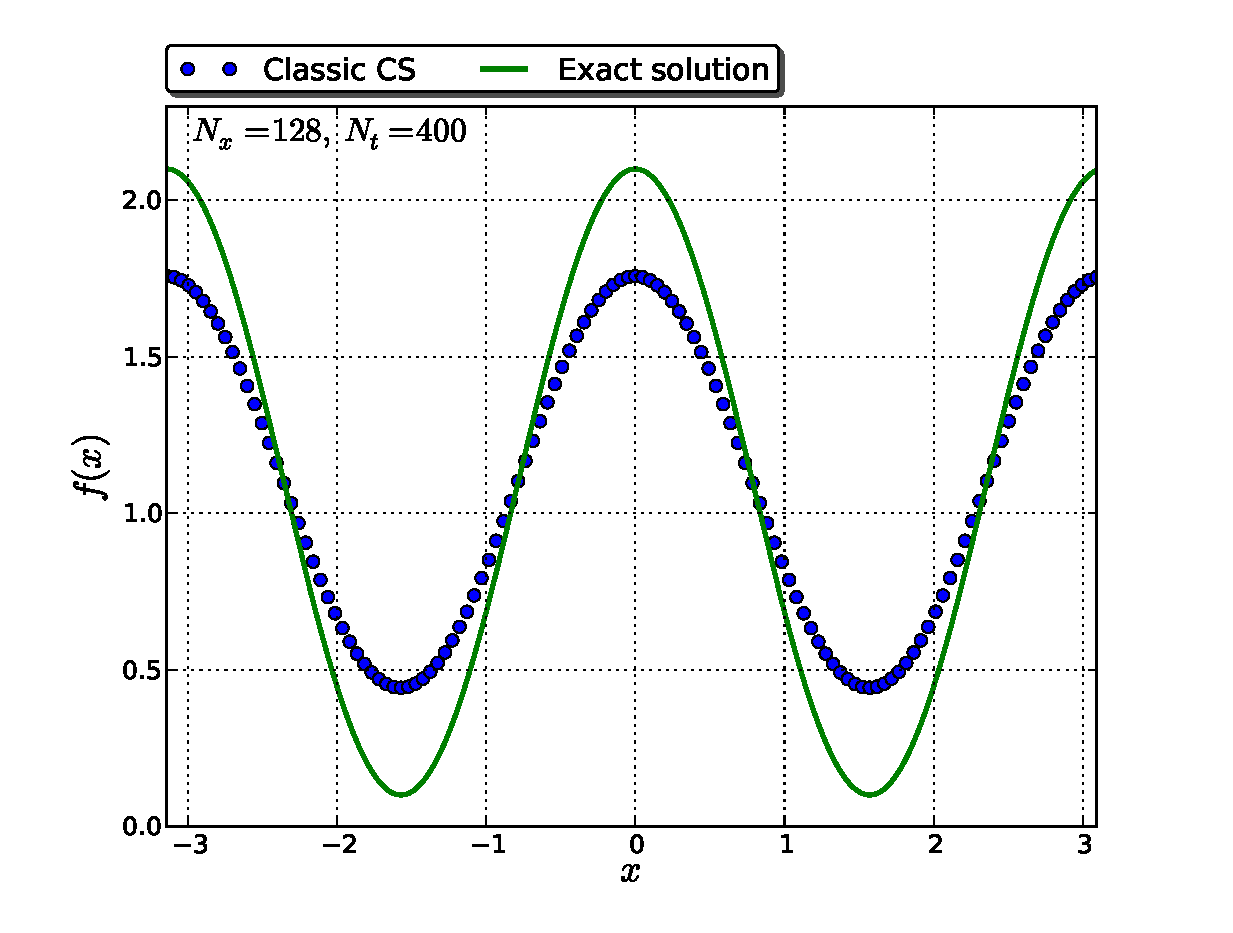
\includegraphics[width=\textwidth]{graphics/plot_-_cos2x_ClassicCS__Nx128Nt400_w_f0_itmax}

  \column{0.52\textwidth}
\begin{tabular}{@{}llll@{}}\toprule
&\multicolumn{3}{c}{\phantom{$^2$ glob }Classic CS} \phantom{Ordera}\\
\cmidrule{2-4}& $\text{NRMS}(\text{GE}_{\Delta x})$ & Order \\ \midrule
$\phantom{a}N_x$\\
$\phantom{a}32$ & $1.4448\phantom{\times 10^{-1}}$ & $-$ \\
$\phantom{a}64$ & $1.0073\phantom{\times 10^{-1}}$ & 0.5204 \\
$\phantom{a}128$ & $6.0739\times 10^{-1}$ & 0.7298 \\
$\phantom{a}256$ & $3.3537\times 10^{-1}$ & 0.8569 \\
$\phantom{a}512$ & $1.7646\times 10^{-1}$ & 0.9264  \\
$\phantom{a}1024$ & $9.0539\times 10^{-2}$ & 0.9626 \\
$\phantom{a}2048$ & $4.5863\times 10^{-2}$ & \textcolor{red}{0.9812} \\
\bottomrule
\end{tabular}

  \end{columns}


\end{frame}

%----------------------------------------------------------------------------------------------------%
%----------------------------------------------------------------------------------------------------%

\begin{frame}{Classic CS: mesh refinement results ($\mathrm{CFL} = 0.32$)}\vspace{-0.2em}
    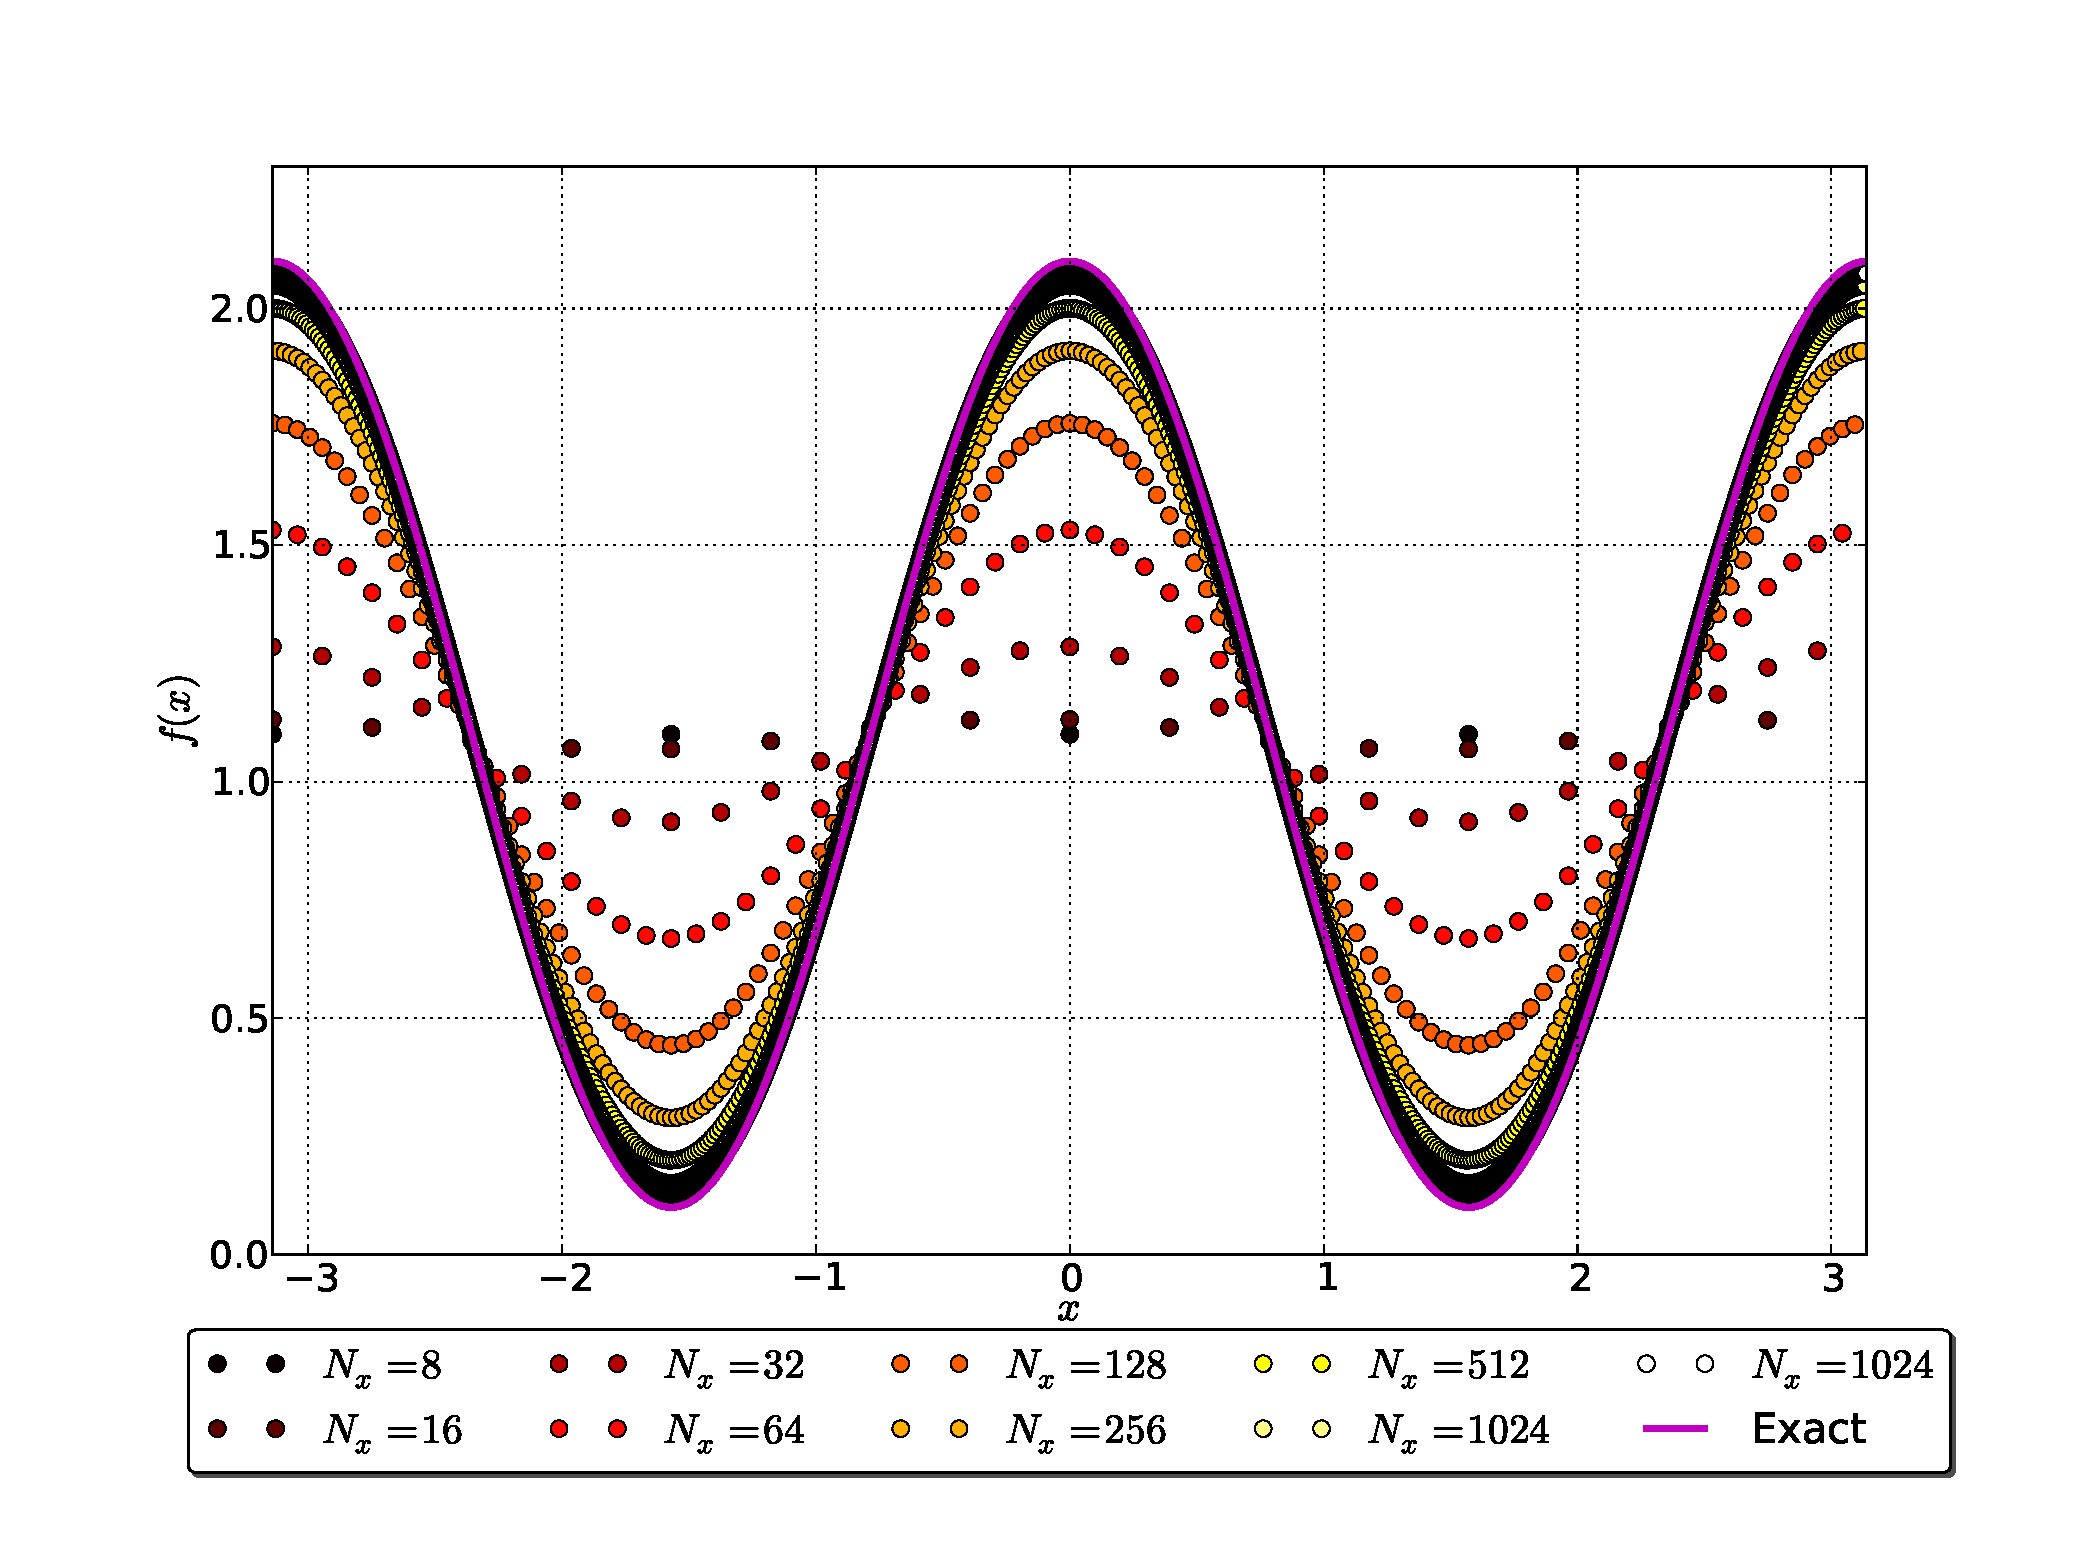
\includegraphics[width=\textwidth]{graphics/plot_-_ClassicCS_cosine2x_Nxall} 
\end{frame}

%----------------------------------------------------------------------------------------------------%
%----------------------------------------------------------------------------------------------------%

\begin{frame}{Classic CS: demonstration} 

\centering [show movie: plot\_-\_cos2x\_ClassicCS\_Nx64Nt200.mpeg and plot\_-\_cos2x\_ClassicCS\_Nx1024Nt3200.mpeg]

\end{frame}

%----------------------------------------------------------------------------------------------------%
%----------------------------------------------------------------------------------------------------%

\begin{frame}{Higher order CS ($FD5$): convergence analysis}
A 5th order CS method with finite differences ($FD5$)\vspace{-0.3em} has been implemented:\vspace{-1em}
$$f_0(x)  = \tfrac{1}{2}e^{-\left(\tfrac{x + 0.2}{0.03}\right)^2} + e^{-\left(\tfrac{x}{0.06}\right)^2} + \tfrac{1}{2}e^{-\left(\tfrac{x - 0.02}{0.03}\right)^2}$$\vspace{-1.5em}
\begin{columns}
  \column{0.48\textwidth}
\begin{tabular}{@{}llll@{}}\toprule
&\multicolumn{3}{c}{\phantom{$^2$ glob }FD5} \phantom{ClasicOrdera}\\
\cmidrule{2-4}& $\text{NRMS}(\text{GE}_{\Delta x})$ & Order \\ \midrule
$\phantom{a}N_x$\\
$\phantom{a}32$ & $7.2912\times 10^{-2}$ & $-$ \\
$\phantom{a}64$ & $2.5443\times 10^{-2}$ & 1.5189 \\
$\phantom{a}128$ & $4.4472\times 10^{-3}$ & 2.5163 \\
$\phantom{a}256$ & $2.1447\times 10^{-4}$ & 4.3741 \\
$\phantom{a}512$ & $7.0343\times 10^{-6}$ & 4.9302  \\
$\phantom{a}1024$ & $2.2142\times 10^{-7}$ & 4.9895 \\
$\phantom{a}2048$ & $6.9307\times 10^{-9}$ & \textcolor{red}{4.9976} \\
\bottomrule
\end{tabular}

  \column{0.65\textwidth}
    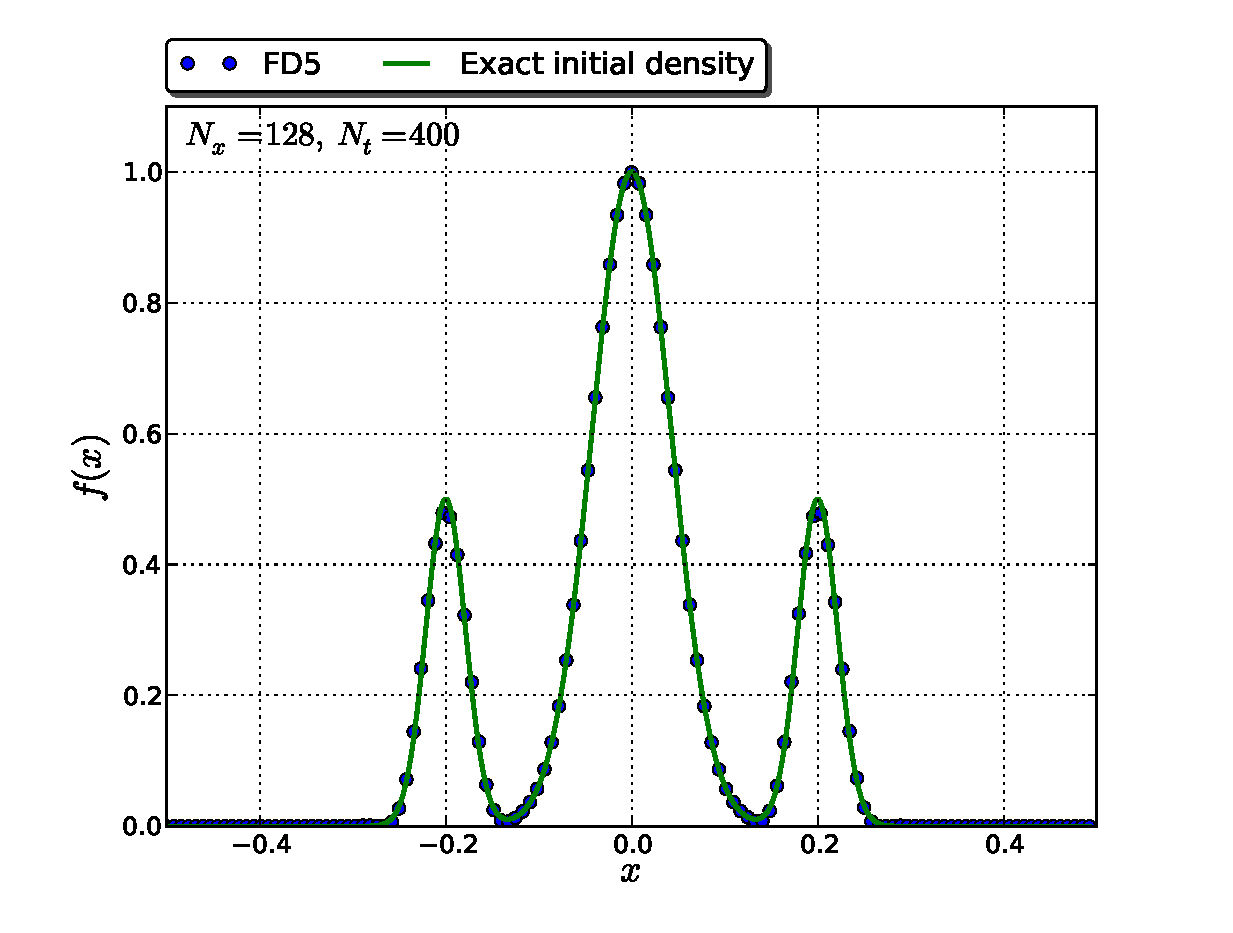
\includegraphics[width=\textwidth]{graphics/plot_-_GB3_FD5__Nx128Nt400_w_f0_itmax.eps}
  \end{columns}

\end{frame}

%----------------------------------------------------------------------------------------------------%
%----------------------------------------------------------------------------------------------------%

\begin{frame}{Higher order CS ($FD5$): mesh refinement ($\mathcal{C} = 0.32$)}\vspace{-0.2em}
    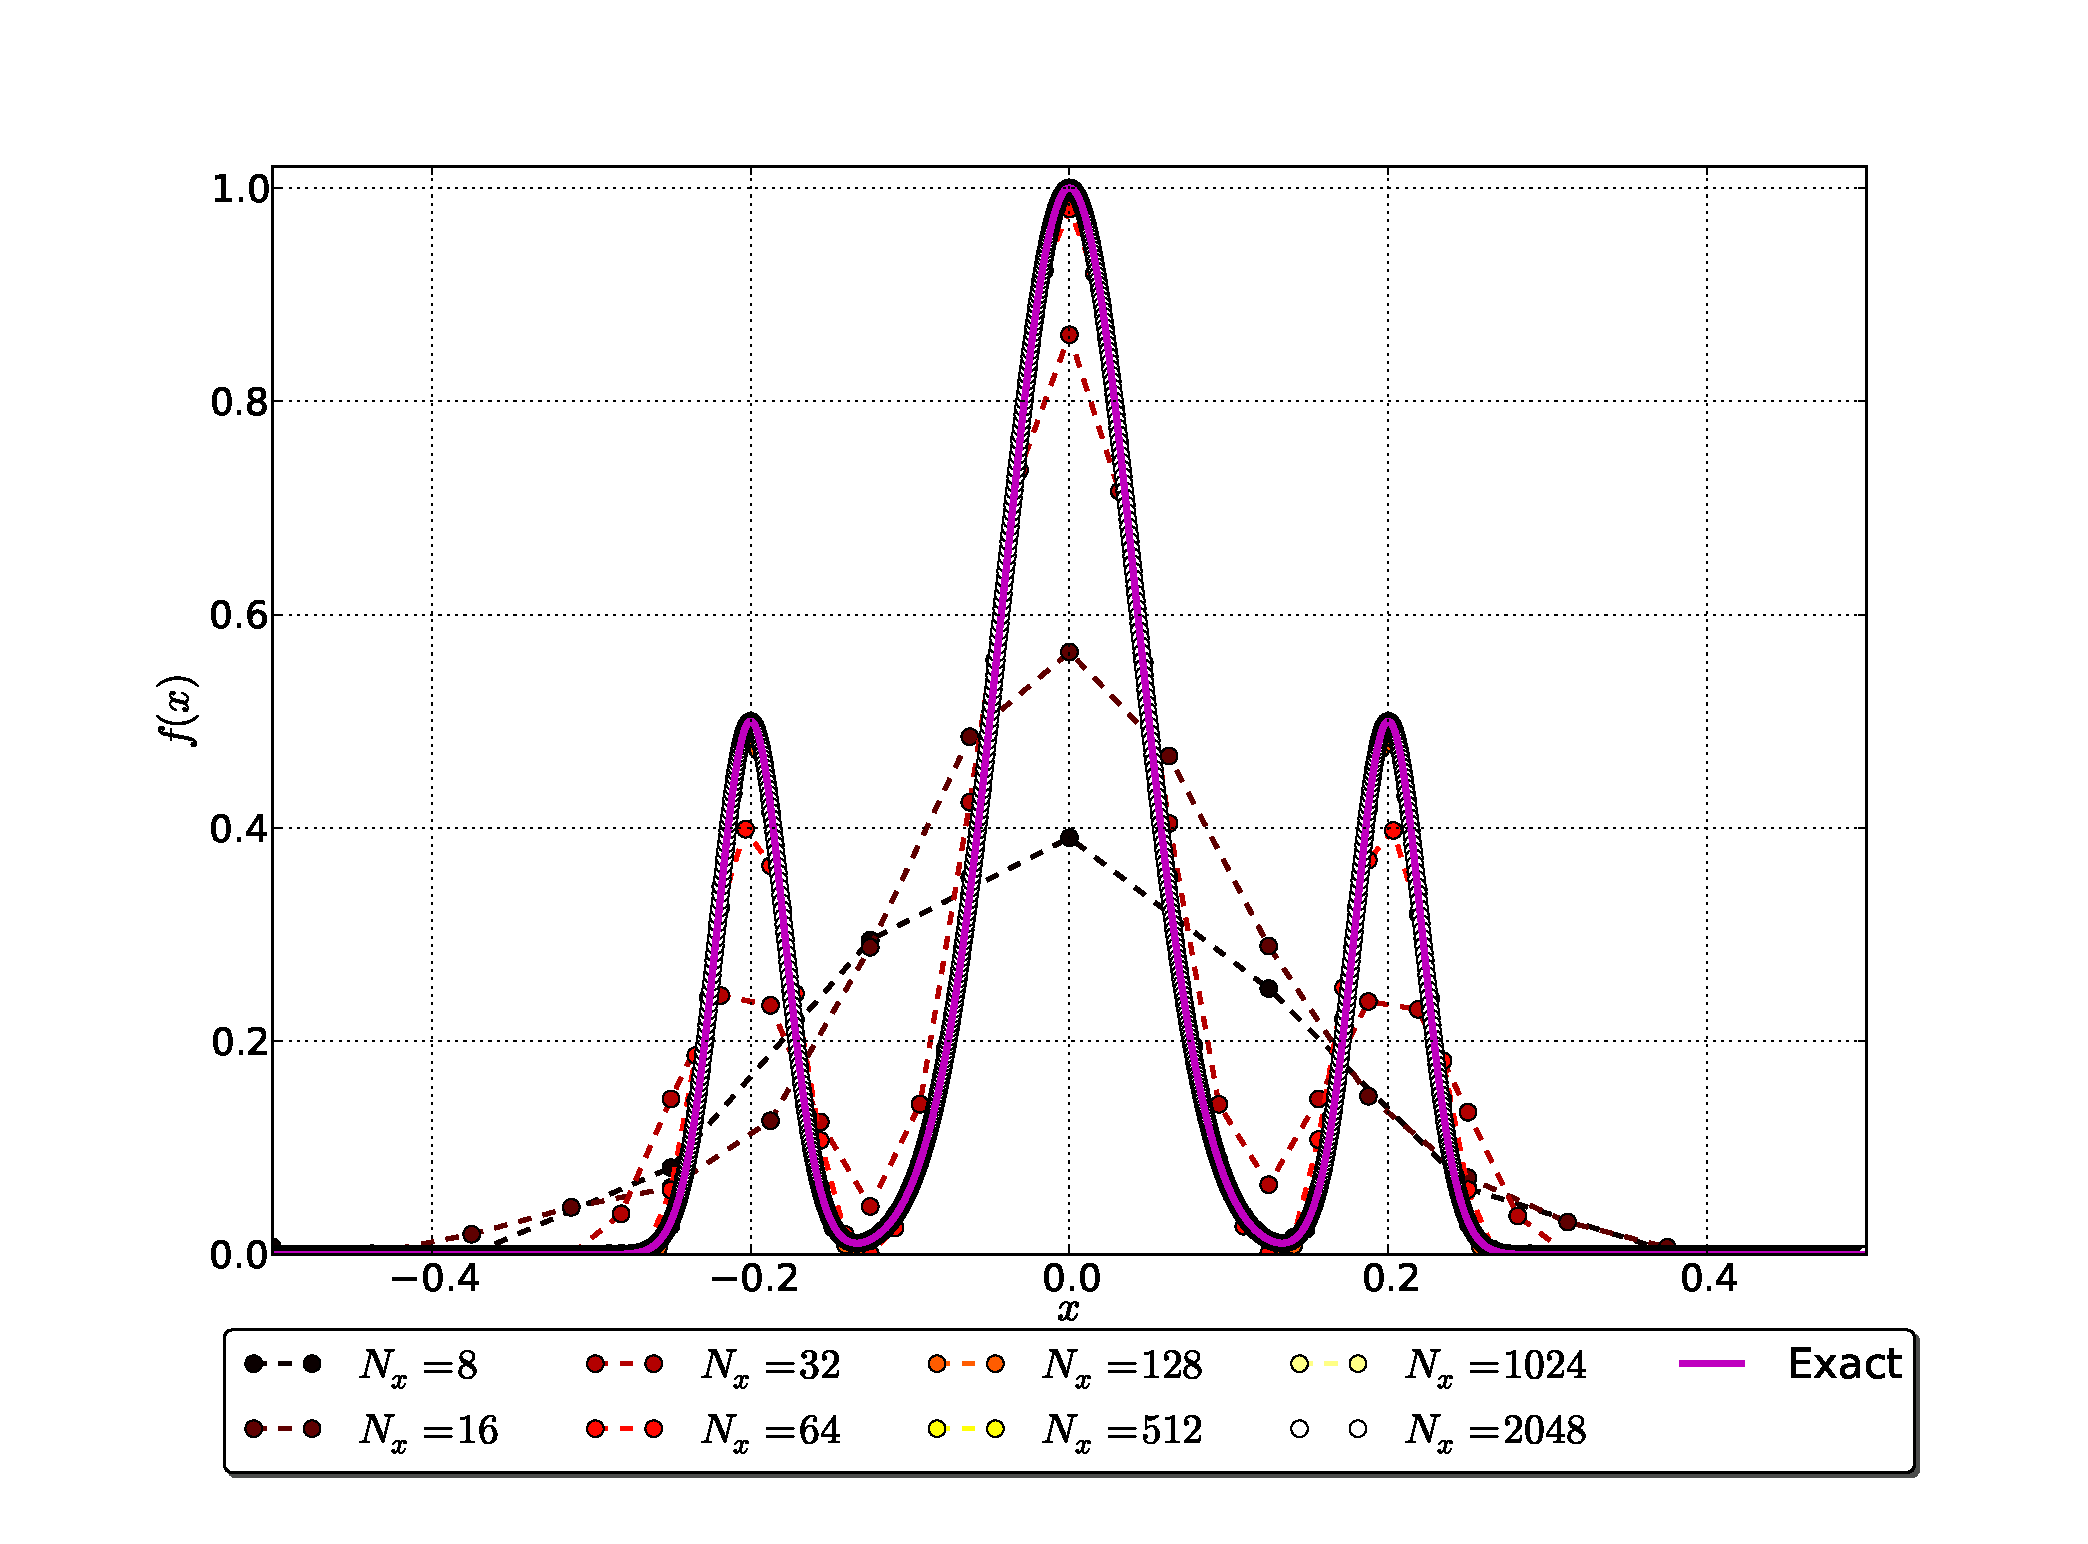
\includegraphics[width=\textwidth]{graphics/plot_-_GB3_FD5_Nxall_dashdot_w_Nx2048}
 
\end{frame}

%----------------------------------------------------------------------------------------------------%
%----------------------------------------------------------------------------------------------------%

\begin{frame}{Higher order CS ($FD5$): demonstration}

\centering  [show movie: plot\_-\_GB3\_FD5\_Nx128Nt400.mpeg]

\end{frame}

%----------------------------------------------------------------------------------------------------%
%----------------------------------------------------------------------------------------------------%

\begin{frame}{Higher order CS ($FN$ methods): various orders $N$}
\vspace*{-5.5mm}
\begin{columns}
  \column{0.5\textwidth}
\begin{figure}
\centering
 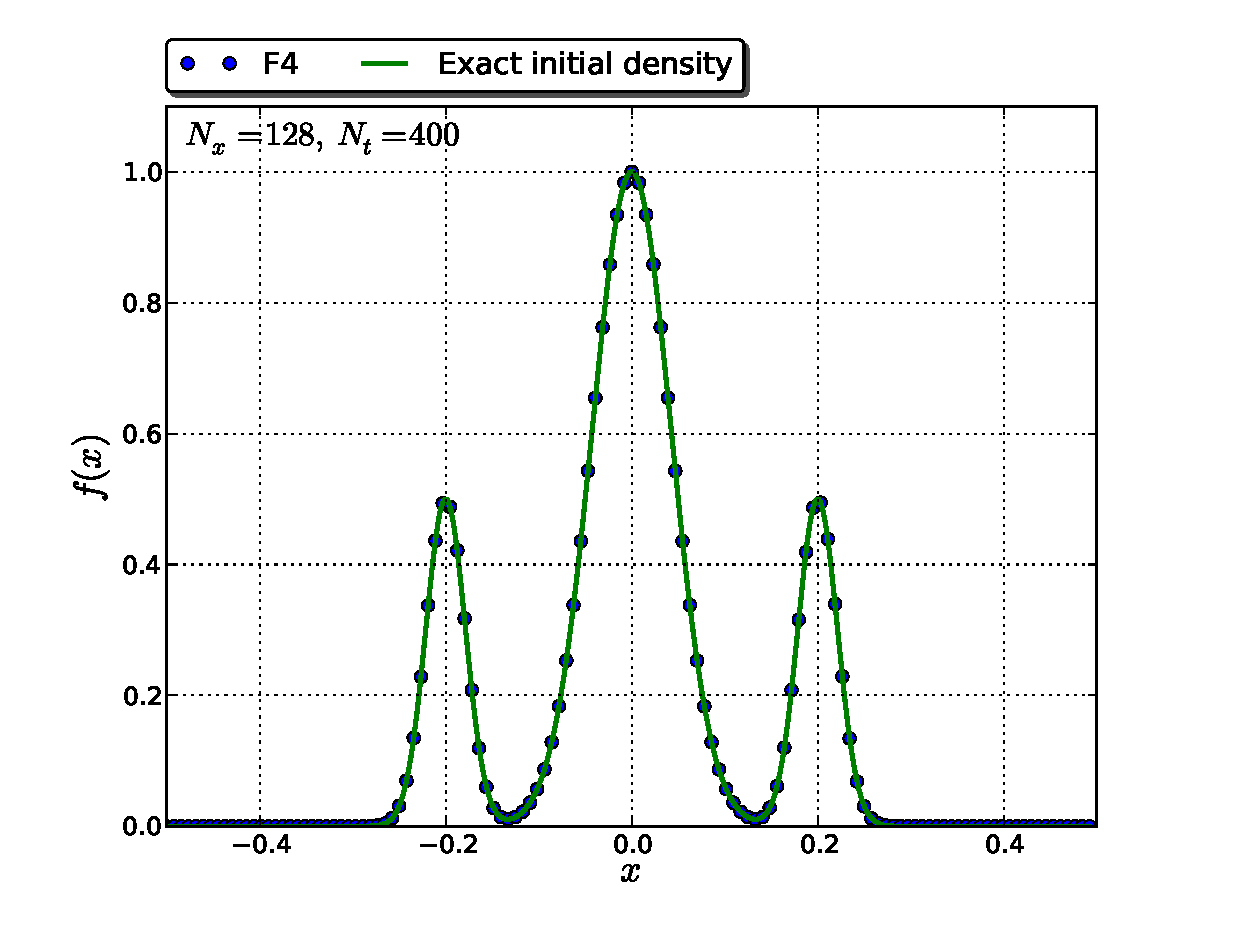
\includegraphics[width=\textwidth]{graphics/plot_-_GB3_F4__Nx128Nt400_w_f0_itmax}\\ \vspace*{-4mm}
 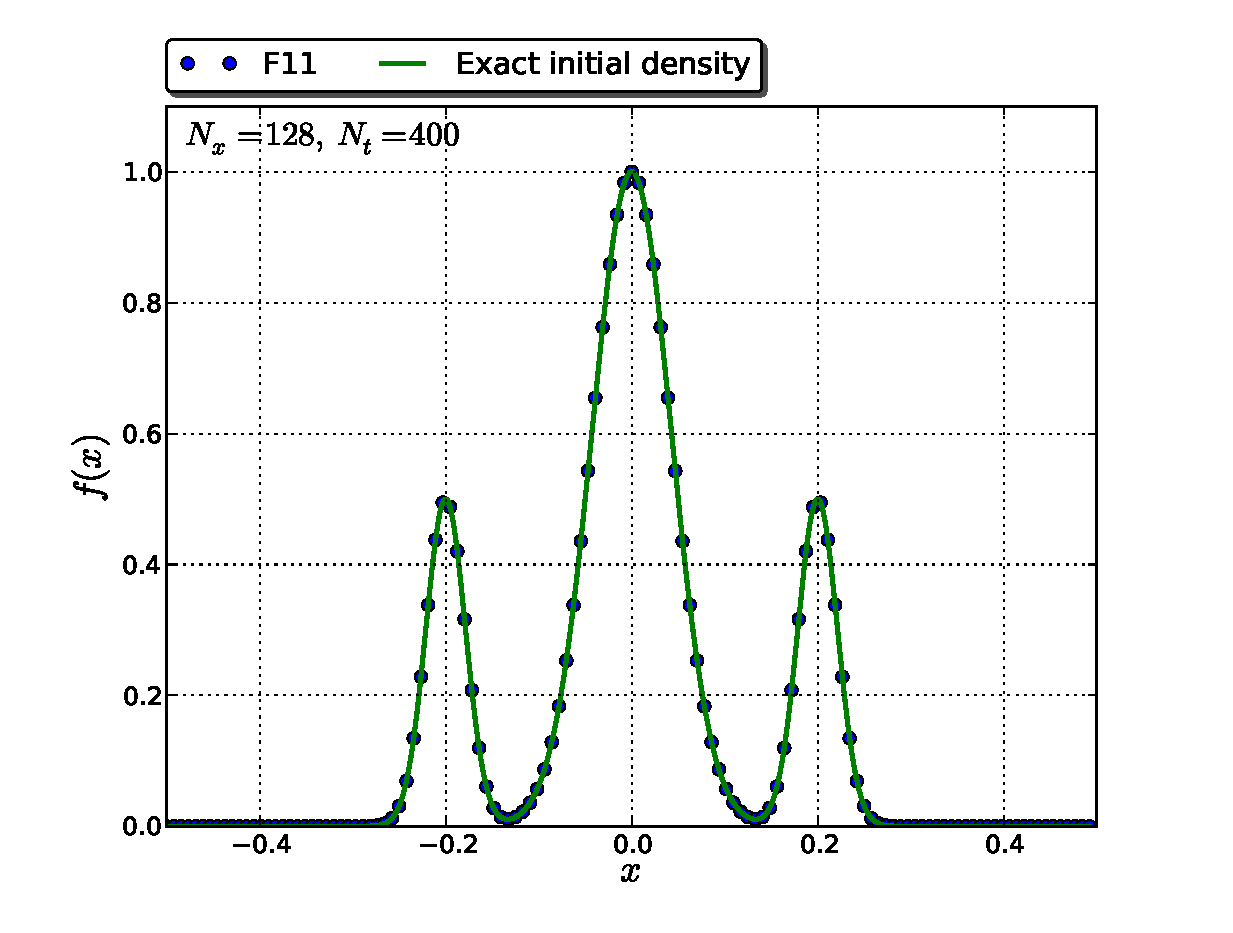
\includegraphics[width=\textwidth]{graphics/plot_-_GB3_F11__Nx128Nt400_w_f0_itmax}
\end{figure}
  \column{0.5\textwidth}
\begin{figure}
\centering
 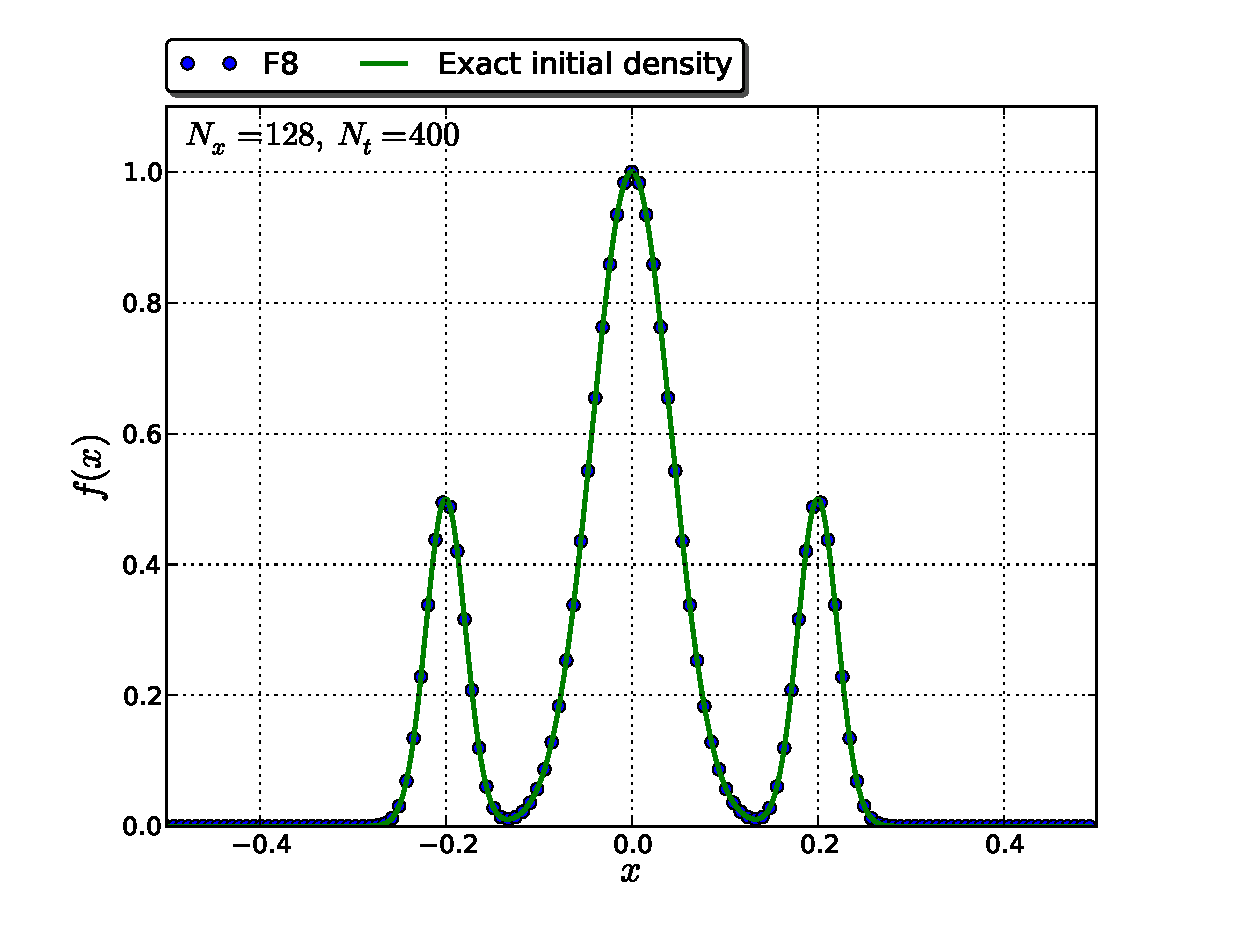
\includegraphics[width=\textwidth]{graphics/plot_-_GB3_F8__Nx128Nt400_w_f0_itmax}\\ \vspace*{-4mm}
 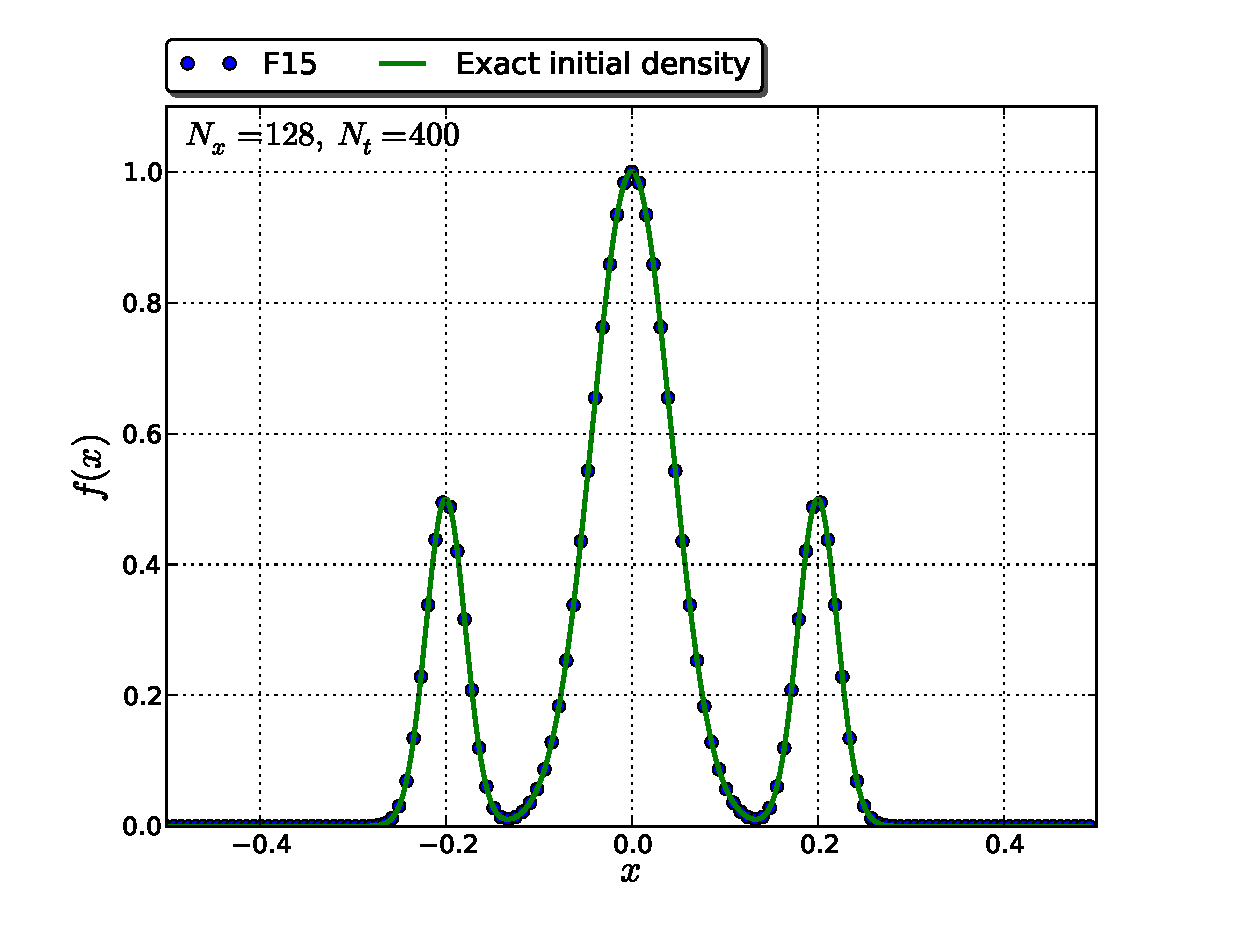
\includegraphics[width=\textwidth]{graphics/plot_-_GB3_F15__Nx128Nt400_w_f0_itmax}
\end{figure}
 \end{columns}
 
\end{frame}

%----------------------------------------------------------------------------------------------------%
%----------------------------------------------------------------------------------------------------%

\begin{frame}

\newcommand\Fontvi{\fontsize{5}{7.2}\selectfont}
\Fontvi
 
\begin{tabular}{@{}lllcllcllcll@{}}\toprule[2 pt]
&\multicolumn{2}{c}{$F2$} & \phantom{a} & \multicolumn{2}{c}{$F3$} &
\phantom{a} & \multicolumn{2}{c}{$F4$} & \\
\cmidrule{2-3} \cmidrule{5-6} \cmidrule{8-9} 
& $\text{NRMS}(\text{GE}_{\Delta x})$ & Order && $\text{NRMS}(\text{GE}_{\Delta x})$ & Order && $\text{NRMS}(\text{GE}_{\Delta x})$ & Order   & \\
\midrule
\phantom{a}$N_x$ \\
\phantom{a}32	&	$9.3763\times 10^{-2}$	&	--	                 	&&	$5.3484\times 10^{-2}$	&	--               		&&	$2.1076\times 10^{-2}$	&	--              		\\
\phantom{a}64	&	$4.7483\times 10^{-2}$	&	0.9816	                 	&&	$1.9892\times 10^{-2}$	&	1.4269           		&&	$4.9206\times 10^{-3}$	&	2.0987            		\\
\phantom{a}128	&	$2.06645\times 10^{-2}$	&	1.2003	                	&&	$4.4207\times 10^{-2}$	&	2.1698		                &&	$3.6497\times 10^{-4}$	&	3.7529            	        \\
\phantom{a}256	&	$6.170\times 10^{-3}$	&	1.7436           		&&	$6.2759\times 10^{-4}$	&	2.8163          		&&	$2.2817\times 10^{-5}$	&	3.9996                          \\
\phantom{a}512	&	$1.5708\times 10^{-3}$	&	\textcolor{red}{1.9739}		&&	$8.0046\times 10^{-5}$	&	\textcolor{red}{2.9709}		&&	$1.4228\times 10^{-6}$	&	\textcolor{red}{4.0032}	        \\	
\midrule
&\multicolumn{2}{c}{$F5$} & \phantom{abc} & \multicolumn{2}{c}{$F6$} &
\phantom{abc} & \multicolumn{2}{c}{$F7$} & \\
\cmidrule{2-3} \cmidrule{5-6} \cmidrule{8-9} 
& $\text{NRMS}(\text{GE}_{\Delta x})$ & Order && $\text{NRMS}(\text{GE}_{\Delta x})$ & Order && $\text{NRMS}(\text{GE}_{\Delta x})$ & Order  & \\
\midrule
\phantom{a}$N_x$ \\
\phantom{a}32	& $1.8251\times 10^{-2}$	&	--	                        && $1.4003\times 10^{-2}$	&	--              		&&	$1.3743\times 10^{-2}$	&	--                 		\\
\phantom{a}64	& $2.0776\times 10^{-3}$	&	3.1350		                && $4.7357\times 10^{-4}$	&	4.8860            		&&	$2.2053\times 10^{-4}$	&	5.9615               	        \\
\phantom{a}128	& $8.0741\times 10^{-5}$	&	4.6855		                && $7.7235\times 10^{-6}$	&	5.9381                		&&	$1.9207\times 10^{-6}$	&	6.8432          		\\
\phantom{a}256	& $2.5658\times 10^{-6}$	&	4.9757	                     	&& $1.1945\times 10^{-7}$	&	\textcolor{red}{6.0147}		&&	$1.5166\times 10^{-8}$	&	\textcolor{red}{6.9847}		\\
\phantom{a}512	& $8.0364\times 10^{-8}$	&	\textcolor{red}{4.9967}	        && $1.8608\times 10^{-9}$	&	6.0042           		&&	--	                &	--              		\\
\midrule
&\multicolumn{2}{c}{$F8$} & \phantom{abc} & \multicolumn{2}{c}{$F9$} &
\phantom{abc} & \multicolumn{2}{c}{$F10$} & \\
\cmidrule{2-3} \cmidrule{5-6} \cmidrule{8-9} 
& $\text{NRMS}(\text{GE}_{\Delta x})$ & Order && $\text{NRMS}(\text{GE}_{\Delta x})$ & Order && $\text{NRMS}(\text{GE}_{\Delta x})$ & Order  & \\
\midrule
\phantom{a}$N_x$ \\
\phantom{a}32	&	$1.3757\times 10^{-2}$	&	--	                  &&  $1.3711\times 10^{-2}$	&	--	    &&    $1.3742\times 10^{-2}$	&	--        \\
\phantom{a}64	&	$5.6229\times 10^{-5}$	&	7.934635	          &&  $3.0591\times 10^{-5}$	&	8.808078	    &&    $1.4822\times 10^{-5}$	&	9.8566    \\
\phantom{a}128	&	$2.1371\times 10^{-7}$	&	\textcolor{red}{8.039495} &&  $5.8963\times 10^{-8}$	&	\textcolor{red}{9.019098}		  &&    $7.3664\times 10^{-9}$	&	10.9745 	\\
\phantom{a}256	&	$8.2396\times 10^{-10}$	&	8.039495                  &&  $1.1657\times 10^{-10}$	&	8.982388		  &&    $7.0799\times 10^{-12}$	&	\textcolor{red}{10.0758}	\\
\phantom{a}512	&	--	                &	--		          &&         --	                &	--		  &&    $1.0180\times 10^{-13}$	&	$(m.p.)$	\\
\bottomrule[2 pt]
\end{tabular}

\end{frame}

%----------------------------------------------------------------------------------------------------%
%----------------------------------------------------------------------------------------------------%

\begin{frame}

\newcommand\Fontvi{\fontsize{7}{7.2}\selectfont}
\Fontvi
\renewcommand\arraystretch{2} 
\hspace*{-6.5mm}\begin{tabular}{@{}lllcllcllcll@{}}\toprule[2 pt]
&\multicolumn{2}{c}{$F11$} & \phantom{a} & \multicolumn{2}{c}{$F12$} &
\phantom{a} & \multicolumn{2}{c}{$F13$}  \\
\cmidrule{2-3} \cmidrule{5-6} \cmidrule{8-9} 
& $\text{NRMS}(\text{GE}_{\Delta x})$ & Order && $\text{NRMS}(\text{GE}_{\Delta x})$ & Order && $\text{NRMS}(\text{GE}_{\Delta x})$ & Order   \\
\midrule
\phantom{a}$N_x$ \\

\phantom{a}32	& $1.3733\times 10^{-2}$	&	--		        &&	$1.3736\times 10^{-2}$	&	--		&&	$1.3734\times 10^{-2}$	&	--	\\
\phantom{a}64	& $1.3397\times 10^{-5}$	&	10.0014		        &&	$1.2761\times 10^{-5}$	&	10.0721		&&	$1.2718\times 10^{-5}$	&	10.0766	\\
\phantom{a}128	& $2.2175\times 10^{-9}$	&	12.5607		        &&	$3.0450\times 10^{-10}$	&	15.3548		&&	$9.8644\times 10^{-11}$	&	16.9763	\\
\phantom{a}256	& $1.1011\times 10^{-12}$	&	10.9758&&	$9.7125\times 10^{-14}$	&	$(m.p.)$		&&	$6.7652\times 10^{-14}$	&	$(m.p.)$	\\
\phantom{a}512	& $1.0180\times 10^{-13}$	&	$(m.p.)$		&&	$1.0187\times 10^{-13}$	&	$(m.p.)$		&&	$1.0182\times 10^{-13}$	&	$(m.p.)$	\\

\bottomrule[2 pt]
\end{tabular}
${}$\\${}$\\
Accuracy achieves machine precision $(m.p.)$ too soon for higher orders to be confirmed
\end{frame}



%----------------------------------------------------------------------------------------------------%
%----------------------------------------------------------------------------------------------------%

\begin{frame}{Challenge case: juxtaposition of all schemes}

Sharp boundaries present challenges to adequately resolve\footnote{G\"{u}\c{c}lu, Y., et al. \emph{Arbitrarily high order convected scheme solution of the Vlasov-Poisson system}. J. Comput. Phys. \textbf{270}, 0 (2014), p.711-752.}
\vspace*{-3mm}
\begin{figure}[h!]
  \centering
    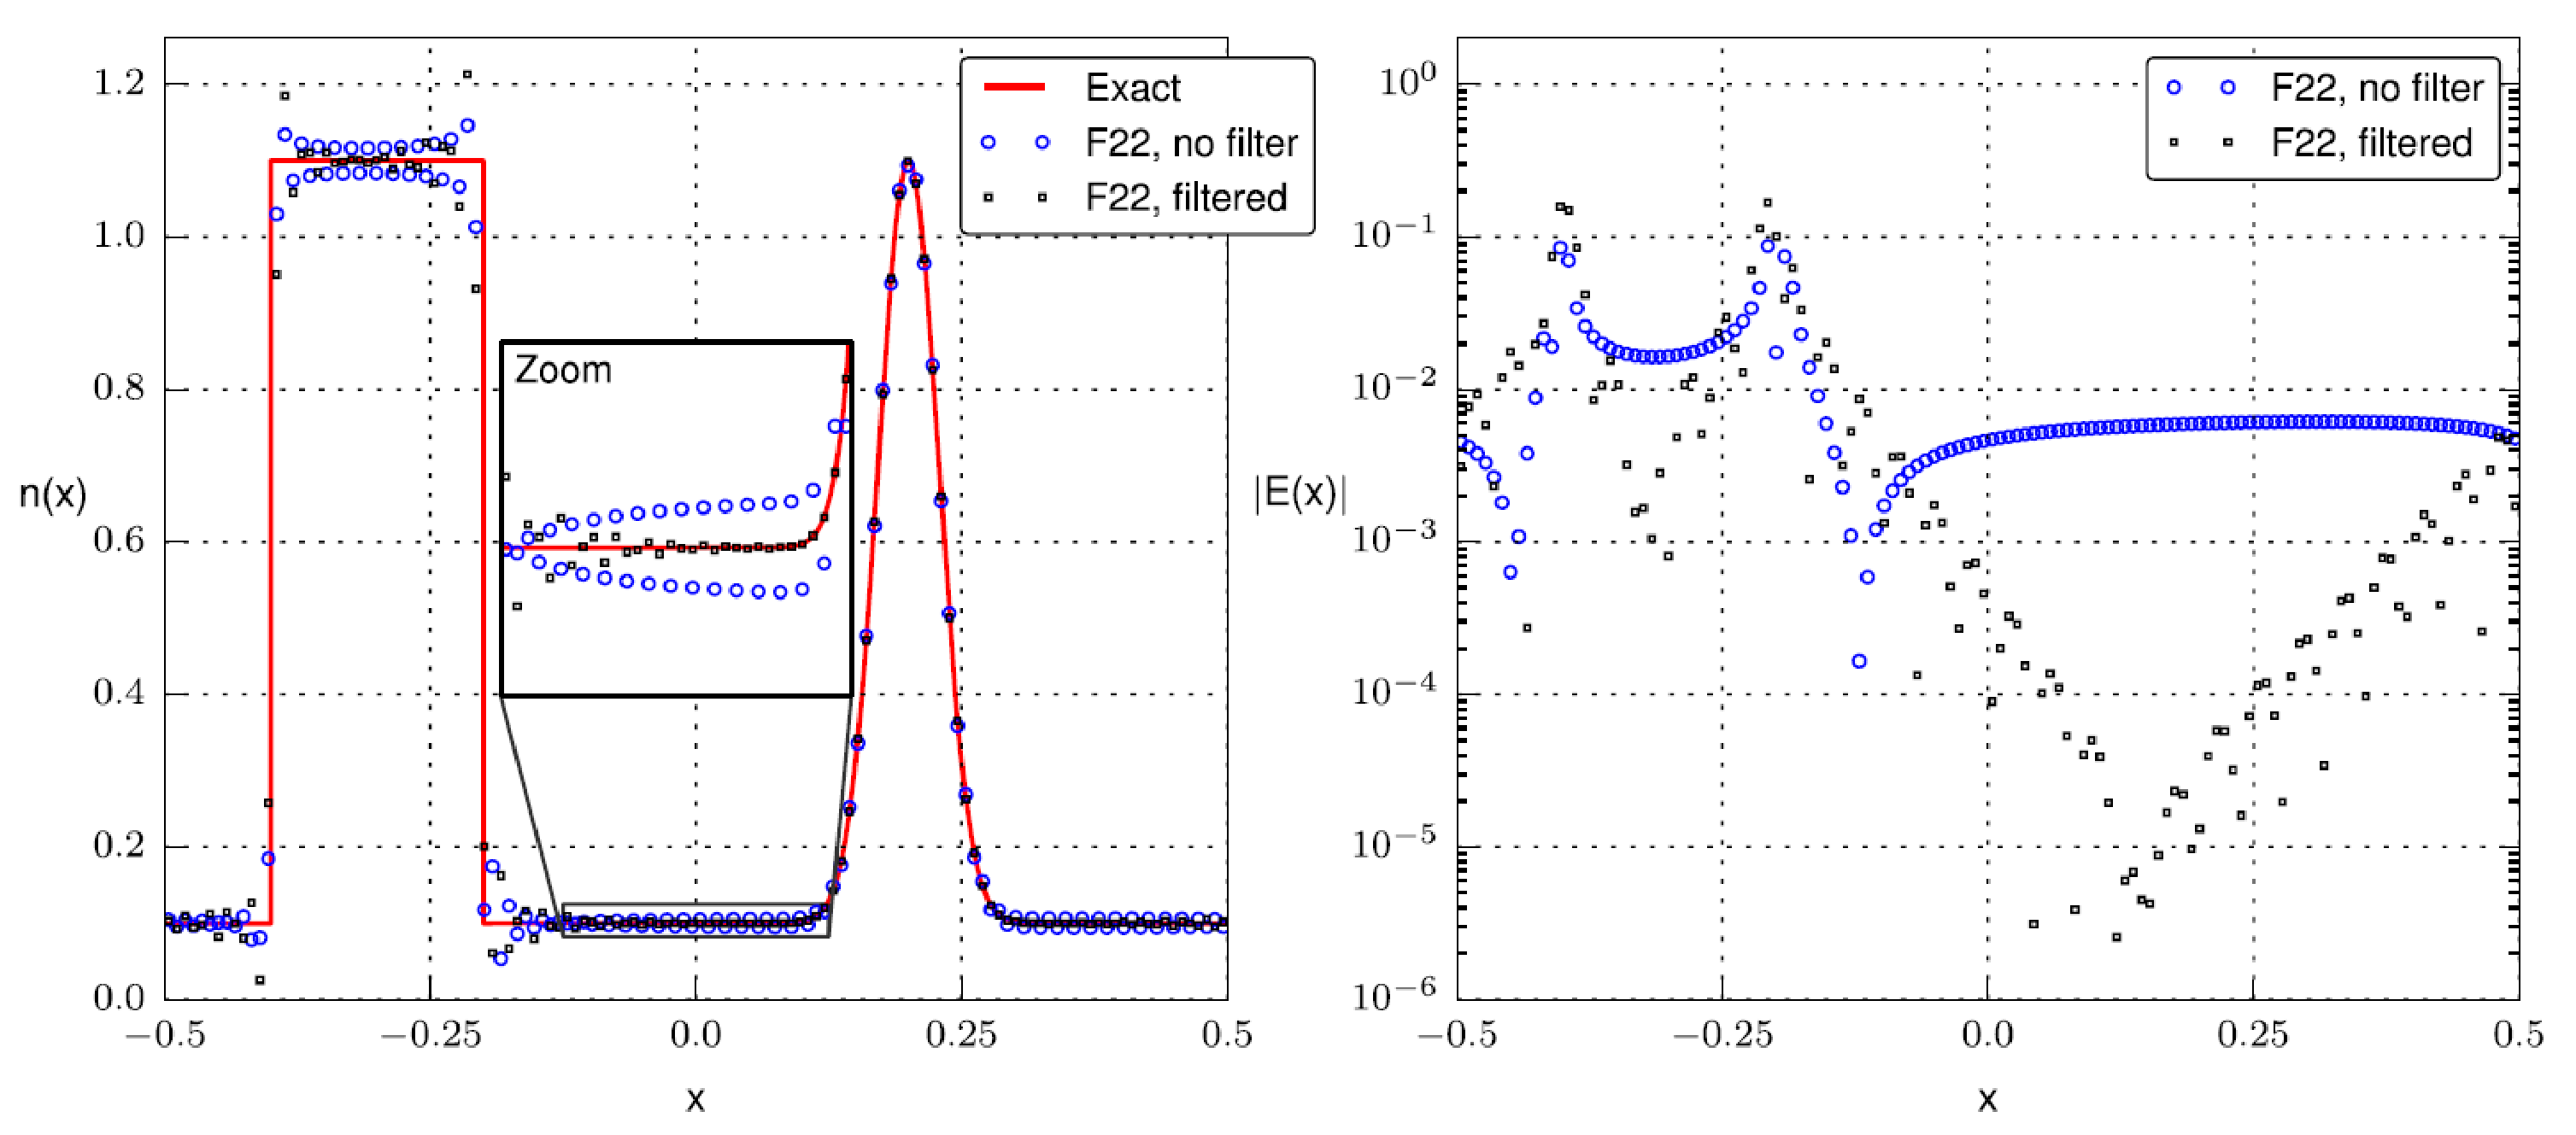
\includegraphics[width=\textwidth]{graphics/WFT_example}
\end{figure}
\vspace*{-5mm}
A windowed Fourier transform (WFT) can be applied to localize the jump errors (cf. preliminary document) 


\end{frame}

%----------------------------------------------------------------------------------------------------%
%----------------------------------------------------------------------------------------------------%

\begin{frame}{1D variable velocity advection solutions}

We now permit the velocity to vary as a function of position
 

$$\frac{\partial f}{\partial t} + v(x)\frac{\partial f}{\partial x} =  0, \qquad x\in\mathcal{D}, t\in [0,T]$$
$$f(0,x) = f_0(x) $$
$$f(t,x + L) = f(t,x)$$

And analyze the initial Gaussian distribution:

$$f_0(x) = e^{-x^2 / (2(0.04)^2)}, \qquad x\in [-0.5, 0.5]$$

With prescribed velocity field:

$$v_S(x) = \sin 2\pi x$$




\end{frame}

%----------------------------------------------------------------------------------------------------%
%----------------------------------------------------------------------------------------------------%

\begin{frame}{Variable velocity: snapshots}
\vspace*{-5.5mm}
\begin{columns}
  \column{0.5\textwidth}
\begin{figure}
\centering
 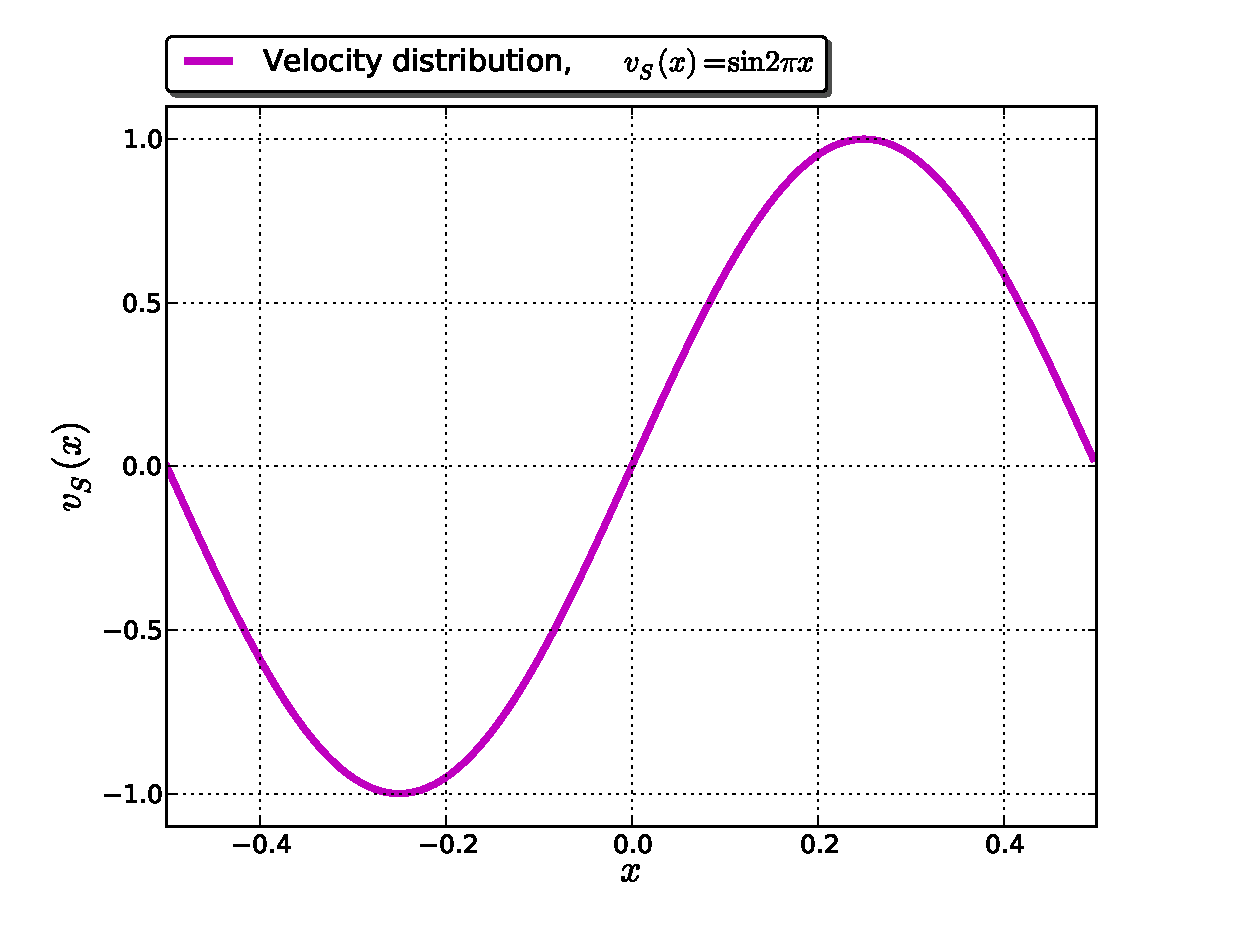
\includegraphics[width=\textwidth]{graphics/v_S_annotated}\\ \vspace*{-4mm}
 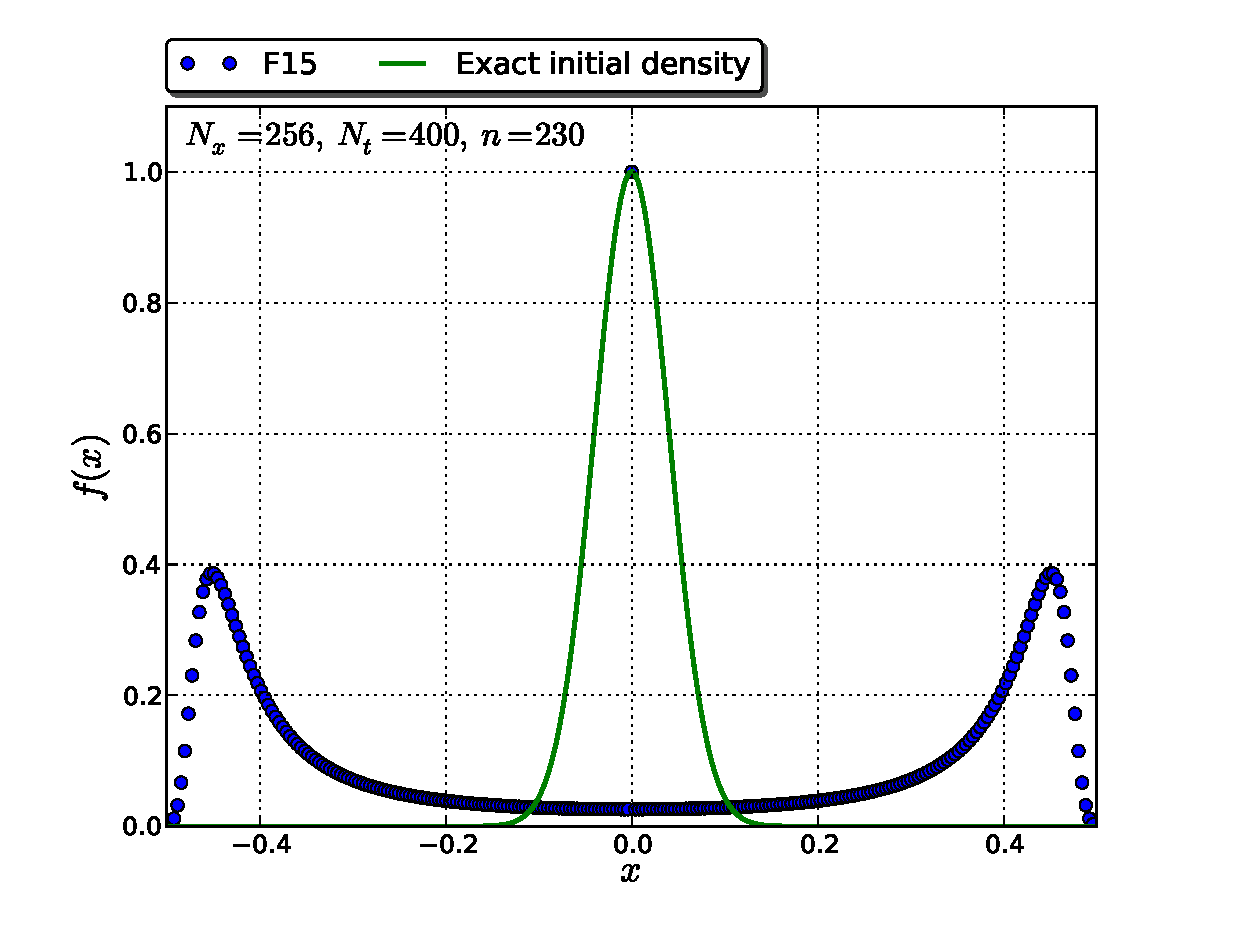
\includegraphics[width=\textwidth]{graphics/f_N_v_S_F15_Nx256Nt400_w_f0_it00230}
\end{figure}
  \column{0.5\textwidth}
\begin{figure}
\centering
 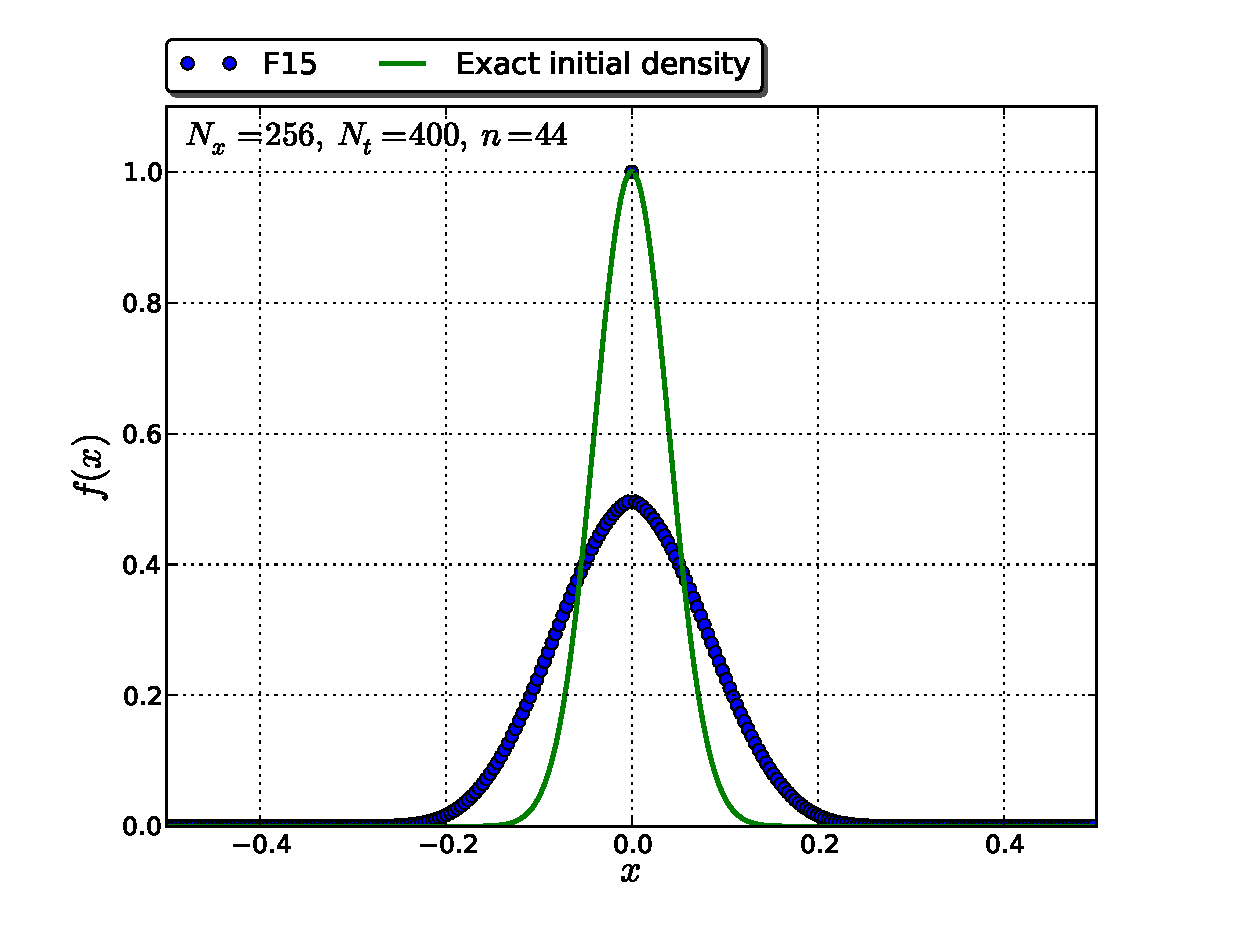
\includegraphics[width=\textwidth]{graphics/f_N_v_S_F15_Nx256Nt400_w_f0_it00044}\\ \vspace*{-4mm}
 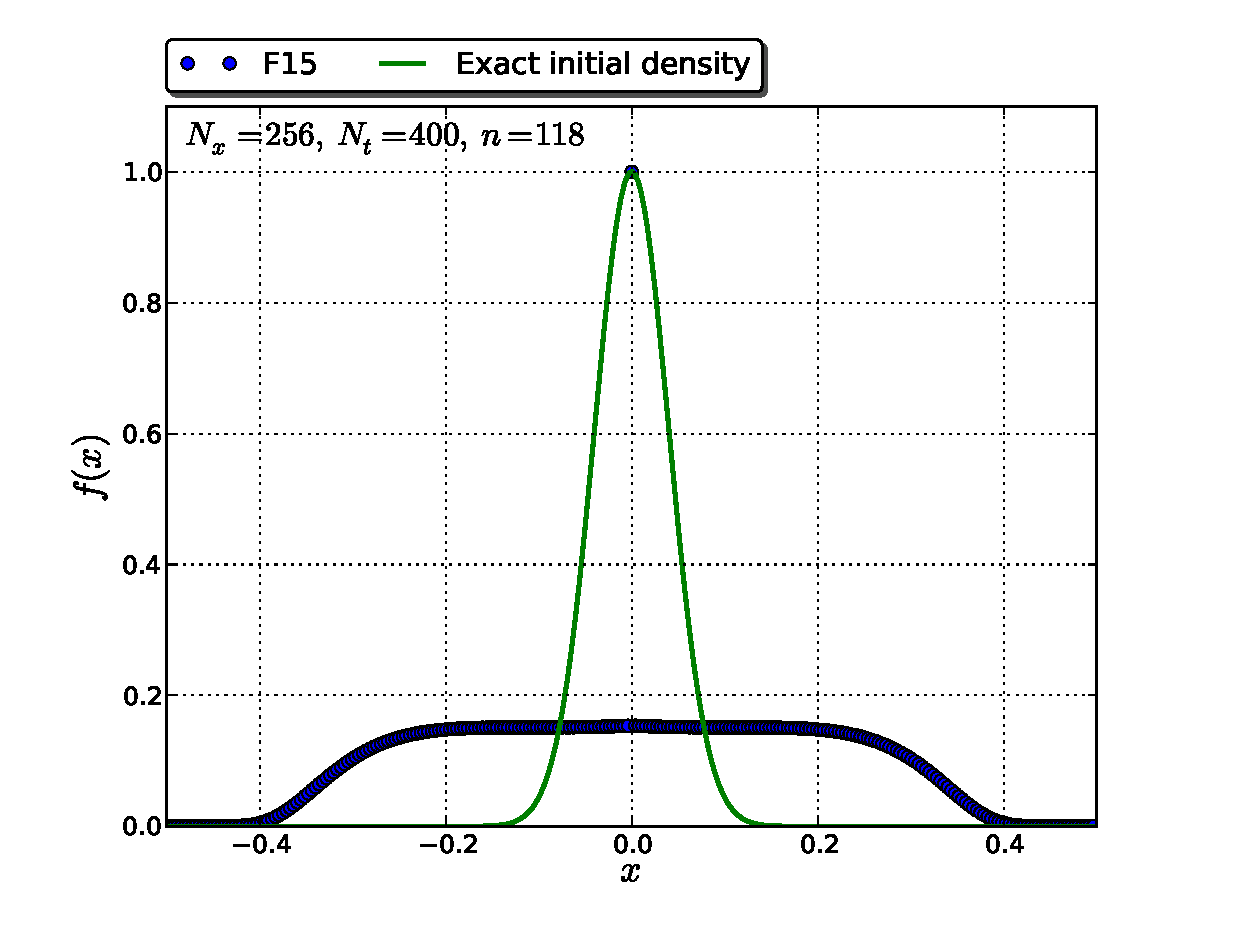
\includegraphics[width=\textwidth]{graphics/f_N_v_S_F15_Nx256Nt400_w_f0_it00118}
\end{figure}
 \end{columns}

\end{frame}

%----------------------------------------------------------------------------------------------------%
%----------------------------------------------------------------------------------------------------%

\begin{frame}{Variable velocity: demonstration}

\centering [show movie: N\_v\_S\_F8\_Nx256Nt400.mpeg]

\end{frame}

%----------------------------------------------------------------------------------------------------%
%----------------------------------------------------------------------------------------------------%

\begin{frame}{Operator splitting methods}
Four split methods were implemented:

\begin{itemize} 
\item \textbf{LF2}\phantom{12} -- 2nd order, 1 stage (\emph{Leapfrog} or \emph{Strang} scheme)
\item \textbf{Y4}\phantom{1-2}\,  -- 4th order, 3 stages (\emph{Yoshida} scheme)
\item \textbf{O6-4}\phantom{1} -- 6th order, optimized, 6 stages (\emph{optimized})
\item \textbf{O11-6} -- 6th order, optimized, 11 stages (\emph{optimized})
\end{itemize}

\blfootnote{Yoshida, H. \emph{Construction of higher order integrators}. Physics letters \textbf{150}, 5,6,7 (1990)}
\blfootnote{Blanes, S. et al. \emph{Practical symplectic partitioned Runge-Kuta and Runge-Kutta-Nystr\"{o}m methods}. J. Comput. and App. Mathe. \textbf{143}, 313--330}

\end{frame}

%----------------------------------------------------------------------------------------------------%
%----------------------------------------------------------------------------------------------------%
\begin{frame}{2D rotating advection equation}

We analyze a 2D rotating advection problem: 

$$\frac{\partial f}{\partial t} + 2\pi y \frac{\partial f}{\partial x} - 2\pi x \frac{\partial f}{\partial y} =  0$$\\[0.3em]
$$(x,y)\in[-1,1]\times [-1,1], \quad t\in [0,1]$$\\[0.3em]
$$f(t,x + L,y) = f(t,x,y),  \quad f(t,x,y+L) = f(t,x,y)$$\\[0.3em]

i.e. the velocities are spatially dependent: 

$$v_x(x,y) = 2\pi y, \quad v_y(x,y) = -2\pi x$$

which describes rotation about $(x_0,y_0) = (0,0)$ with constant angular velocity $\omega = 2\pi$ and period 1.


\end{frame}

%----------------------------------------------------------------------------------------------------%
%----------------------------------------------------------------------------------------------------%
\begin{frame}{2D rotating advection: initial distribution}

The initial distribution we consider is:

$$f_0(x,y) = 0.5 B(r_1(x,y)) + 0.5 B(r_2(x,y))$$

\begin{columns}
\column{0.5\textwidth}
\hspace*{-5mm}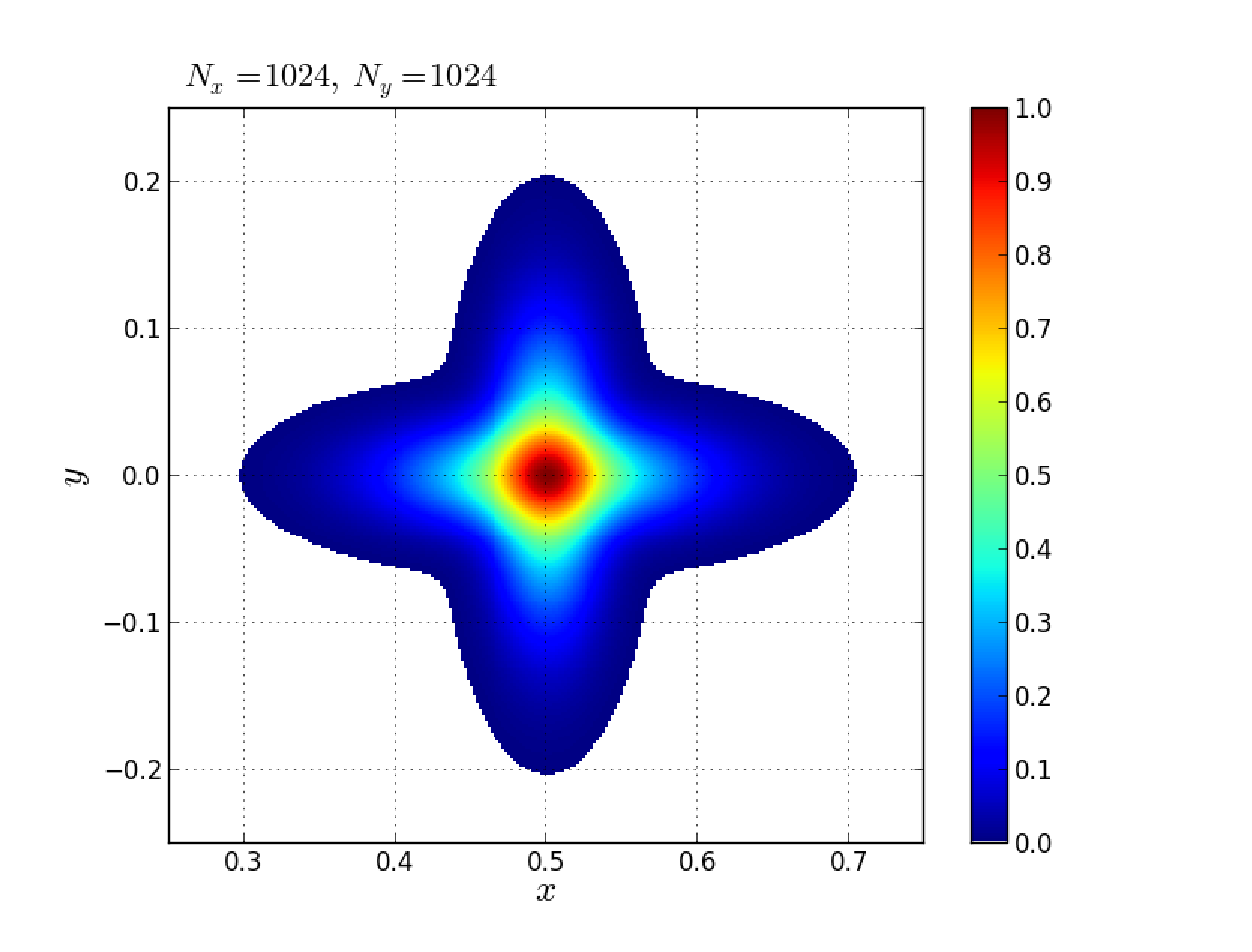
\includegraphics[scale = 0.35]{graphics/f0_2drot_exact_highres}
\column{0.5\textwidth}
\vspace*{-5mm}$$ B(r,a) =
  \begin{cases}
  \cos^{22}\left(\tfrac{\pi r}{2a}\right) & \text{for } r \leq a \\[0.5em]
   0       & \text{else }
  \end{cases}$$

\vspace*{-3mm}
 
$$r_1(x,y) = \sqrt{ (x - x_c)^2 + 8(y - y_c)^2}$$
$$r_2(x,y) = \sqrt{ 8(x - x_c)^2 + (y - y_c)^2}$$
$$2a = 1, \quad (x_c, y_c) = (0,0.5)$$
\end{columns}

\end{frame}

%----------------------------------------------------------------------------------------------------%
%----------------------------------------------------------------------------------------------------%
\begin{frame}{2D rotating advection: snapshots}

\vspace*{-5.5mm}
\begin{columns}
  \column{0.5\textwidth}
\begin{figure}
\centering
 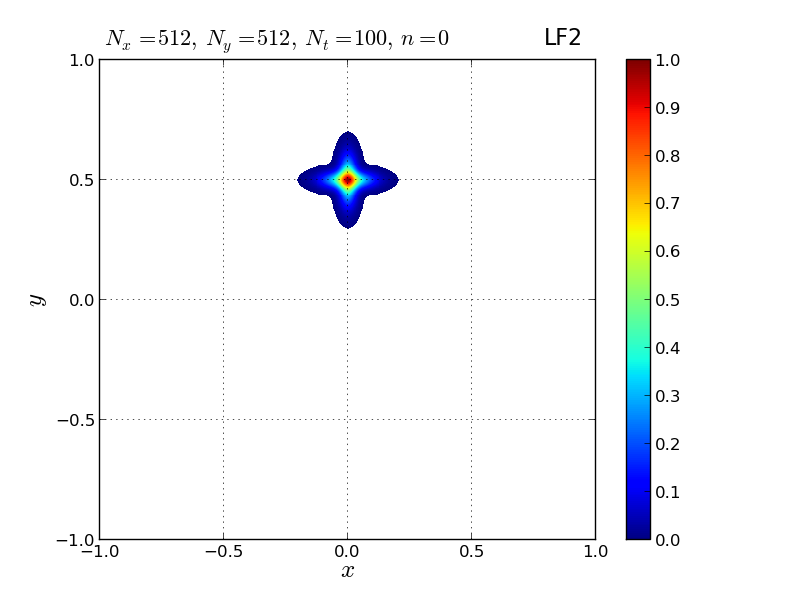
\includegraphics[width=\textwidth]{graphics/plot_-_flower_F12_LF2_Nx512Nt100_it00000}\\ \vspace*{-4mm}
 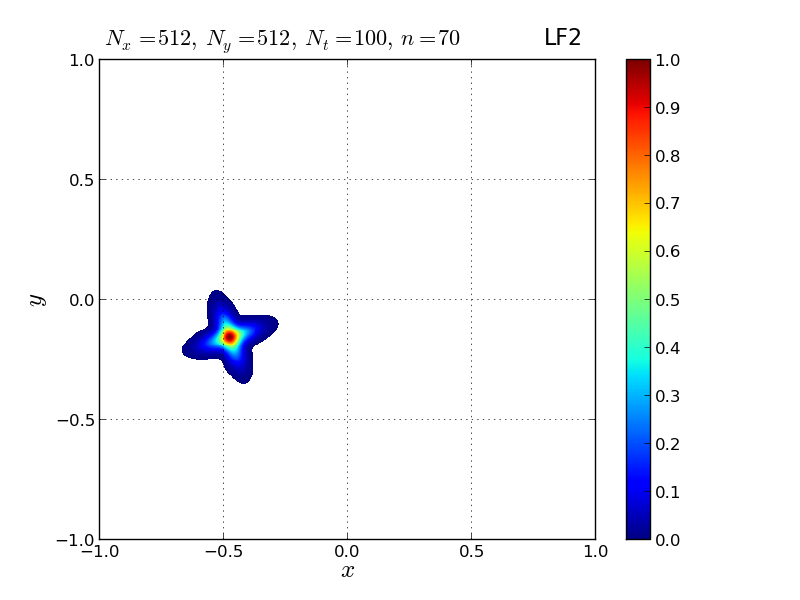
\includegraphics[width=\textwidth]{graphics/plot_-_flower_F12_LF2_Nx512Nt100_it00070}
\end{figure}
  \column{0.5\textwidth}
\begin{figure}
\centering
 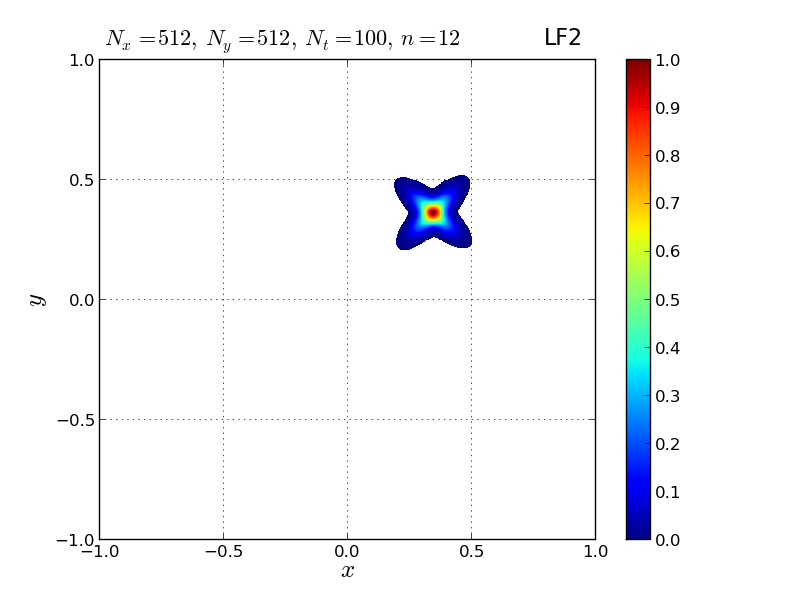
\includegraphics[width=\textwidth]{graphics/plot_-_flower_F12_LF2_Nx512Nt100_it00012}\\ \vspace*{-4mm}
 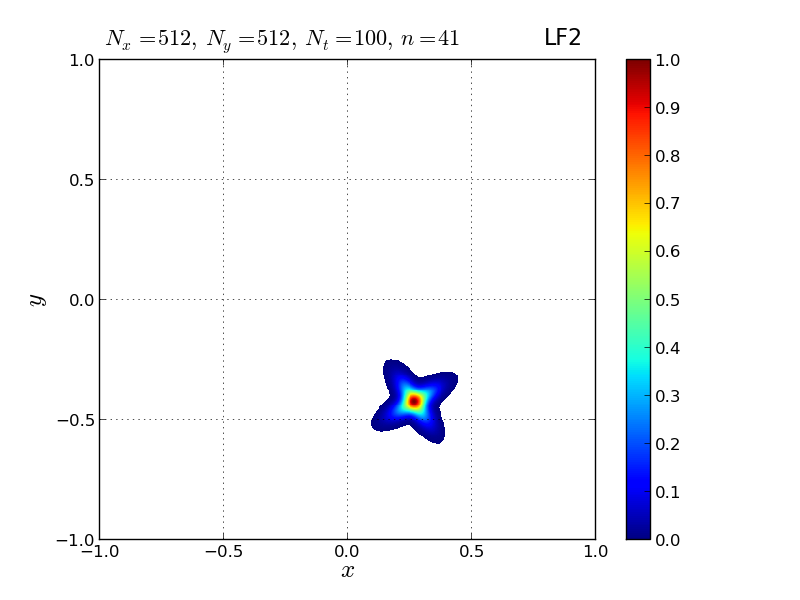
\includegraphics[width=\textwidth]{graphics/plot_-_flower_F12_LF2_Nx512Nt100_it00041}
\end{figure}
 \end{columns}

\end{frame}

%----------------------------------------------------------------------------------------------------%
%----------------------------------------------------------------------------------------------------%
\begin{frame}{2D rotating advection: errors in different split schemes}

\centering [show movie: plot\_-\_flower\_F12\_LF2\_Nx512Nt100.mpeg]
\end{frame}

%----------------------------------------------------------------------------------------------------%
%----------------------------------------------------------------------------------------------------%
\begin{frame}{2D rotating advection: errors in different split schemes}

The $\mathrm{NRMS(GE_{\Delta x, \Delta y})}$ in 2D is the Frobenius norm $||\cdot ||_F$ normalized by the area $|\mathcal{D}_x||\mathcal{D}_y|$.
CS solver was the $F12$ scheme.

\begin{columns}
\column{0.5\textwidth}
\hspace*{-5mm}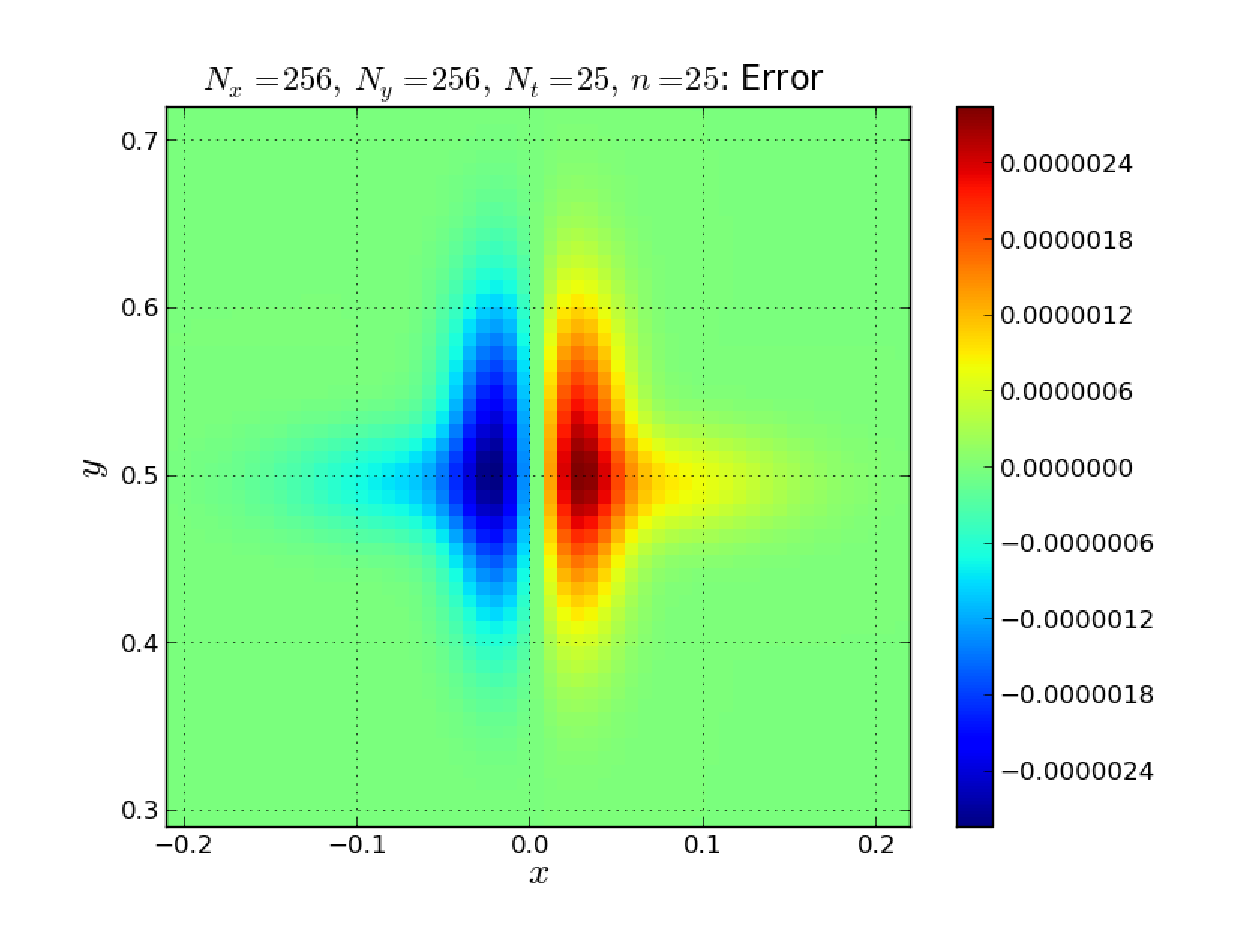
\includegraphics[scale = 0.35]{graphics/Error_closeup8}
\column{0.5\textwidth}
\hspace*{4mm}\begin{tabular}{@{}llll@{}}\toprule
& $\mathrm{NRMS(GE_{\Delta x, \Delta y})}$ \\ \midrule
$\phantom{a}$Scheme\\
$\phantom{a}LF2$ & $4.5338\times 10^{-3}$ \\
$\phantom{a}Y4$ & $1.4368\times 10^{-3}$ \\
$\phantom{a}O6$-4 & $2.1483\times 10^{-5}$ \\
$\phantom{a}O11$-6 & $3.9634\times 10^{-7}$ \\
\bottomrule
\end{tabular}
\end{columns}

\end{frame}

%----------------------------------------------------------------------------------------------------%
%----------------------------------------------------------------------------------------------------%

\begin{frame}{1D-1V Vlasov equation: prescribed $\vec{E}$-field}

Setup:
\begin{itemize}
\item Trapped electrons ($q = -e$) are simulated in a prescribed electric ($\vec{E}$) field as governed by the \emph{Vlasov} equation.
\item normalize according to
    \begin{itemize}
    \item $t \rightarrow t / \tau,$ where $\tau^{-1} = \omega_{pe} / 2\pi$\\[0.5em]
    \item $x \rightarrow x / \lambda_D$\\[0.5em]
    \item $v \rightarrow v / v_{Te} = v / (\lambda_D\omega_{pe})$\\[0.5em]
    \item $E \rightarrow E / \bar{E}$, where $\bar{E} = \tfrac{1}{2}m_ev_{Te}^2 / q \cdot \omega_{pe}$  \\[0.5em]
    \item $f \rightarrow f / \bar{f}$, where $\bar{f} = \langle f \rangle_{v} / v_{Te}^3$
    \end{itemize}

\item Recall $E = -\partial_x \phi$
\end{itemize}

Then the Vlasov equation takes the form:

$$\frac{\partial f}{\partial t} + v\frac{\partial f}{\partial x} + \frac{\partial\phi}{\partial x}\frac{\partial f}{\partial v} = 0$$

\end{frame}

%----------------------------------------------------------------------------------------------------%
%----------------------------------------------------------------------------------------------------%

\begin{frame}{1D-1V Vlasov equation: prescribed $\vec{E}$-field}

$$\frac{\partial f}{\partial t} + v\frac{\partial f}{\partial x} + \frac{\partial\phi}{\partial x}\frac{\partial f}{\partial v} = 0$$

Trapped electrons are simulated with the $F12$ CS by considering the potential:
\vspace*{-2mm}
$$\phi(x) = 0.2 + 0.2\cos(\pi x^4) + 0.1\sin(\pi x)$$
\vspace*{-2mm}
\begin{columns}
\column{0.5\textwidth}
\hspace*{-5mm}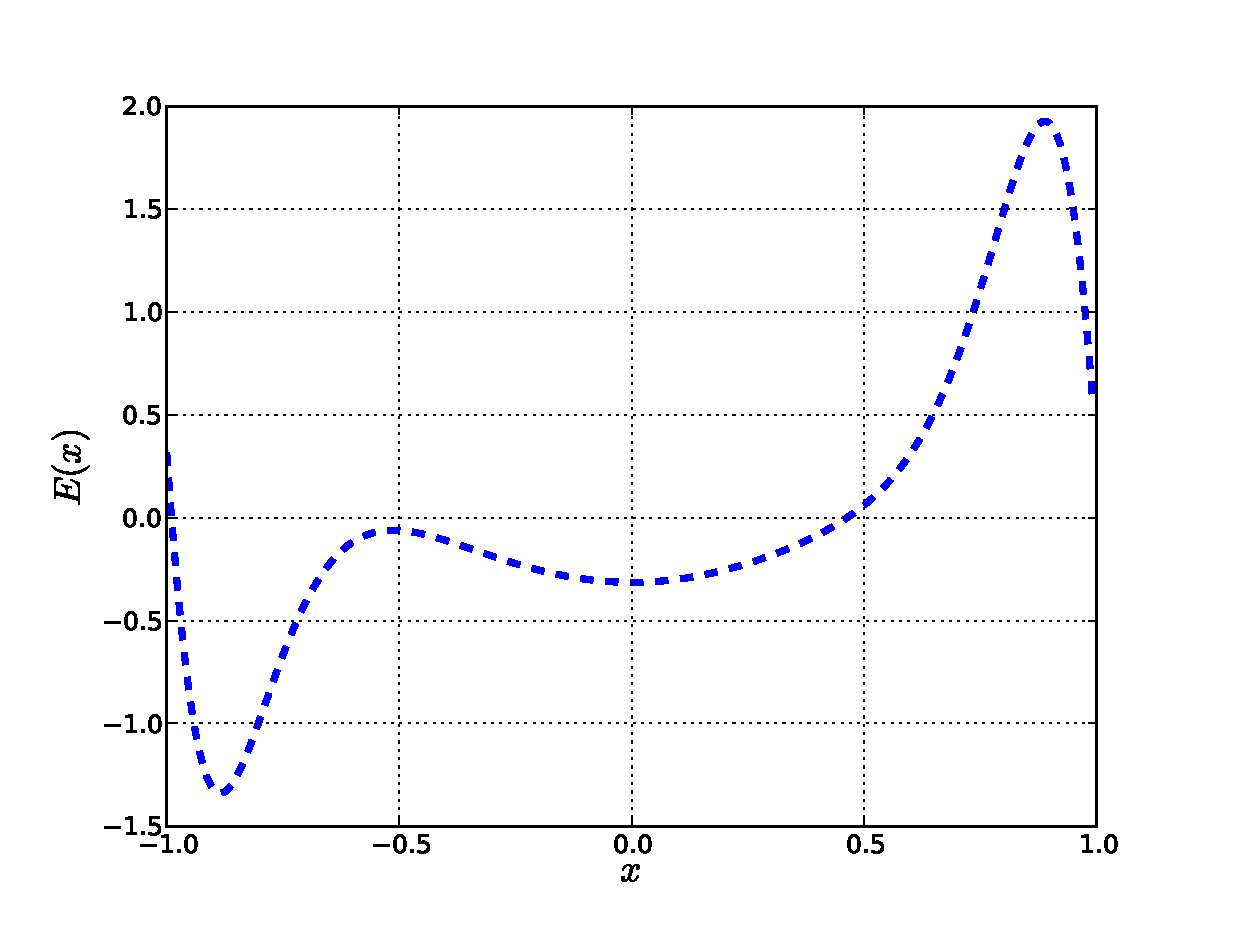
\includegraphics[width = \columnwidth]{graphics/E}
\column{0.5\textwidth} 
\hspace*{-5mm}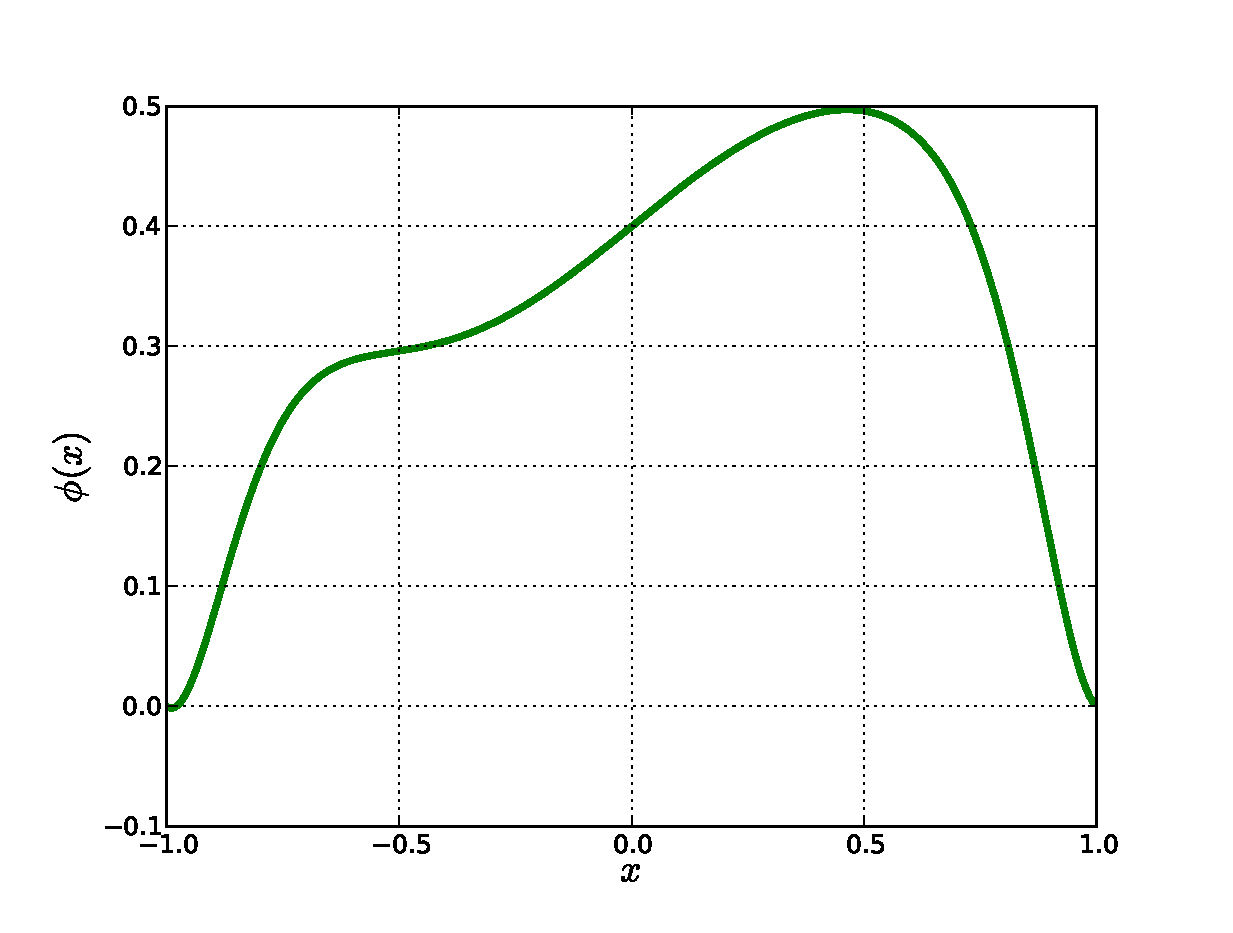
\includegraphics[width = \columnwidth]{graphics/phi}
\end{columns} 

over a simulation time $0 \leq t \leq 6.4$

\end{frame}

%----------------------------------------------------------------------------------------------------%
%----------------------------------------------------------------------------------------------------%
\begin{frame}{1D-1V Vlasov equation: prescribed $\vec{E}$-field}

Initial distribution

\begin{columns}
\column{0.5\textwidth}
$$ B(r,a) =
  \begin{cases}
  \cos^{22}\left(\tfrac{\pi r}{2a}\right) & \text{for } r \leq a \\
   0       & \text{else }
  \end{cases}$$
\vspace*{-3.5mm}
$$r = \sqrt{(x - x_c)^2 + (v - v_c)^2}$$ 
\column{0.5\textwidth}
The Hamiltonian is constant:
$$H = \frac{1}{2}v_0^2 - \phi (x_0) = \frac{1}{2}v(t)^2 - \phi (x(t))$$
\end{columns}
 

\begin{columns}
\column{0.5\textwidth}
\hspace*{-5mm}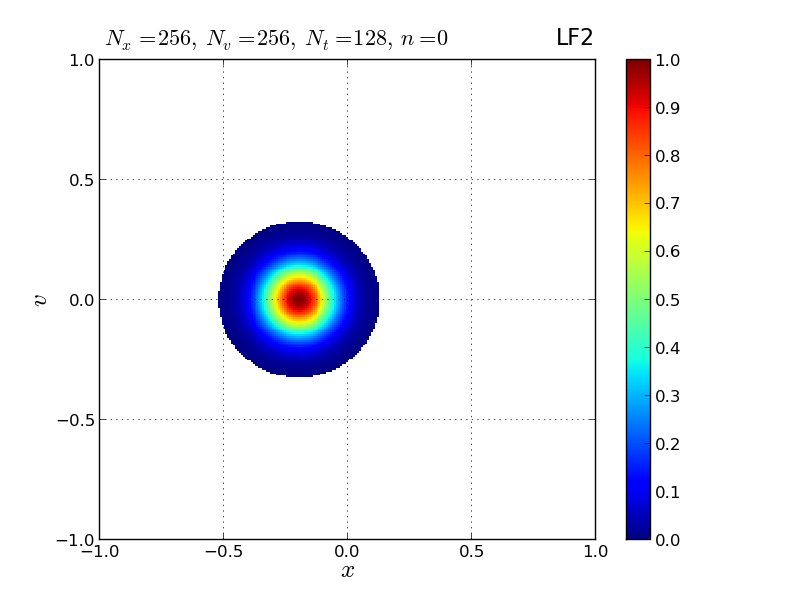
\includegraphics[scale = 0.30]{graphics/plot_-_1DVP_F12_Nx256Nv256Nt128_it00000}
\column{0.5\textwidth}
\hspace*{-5mm}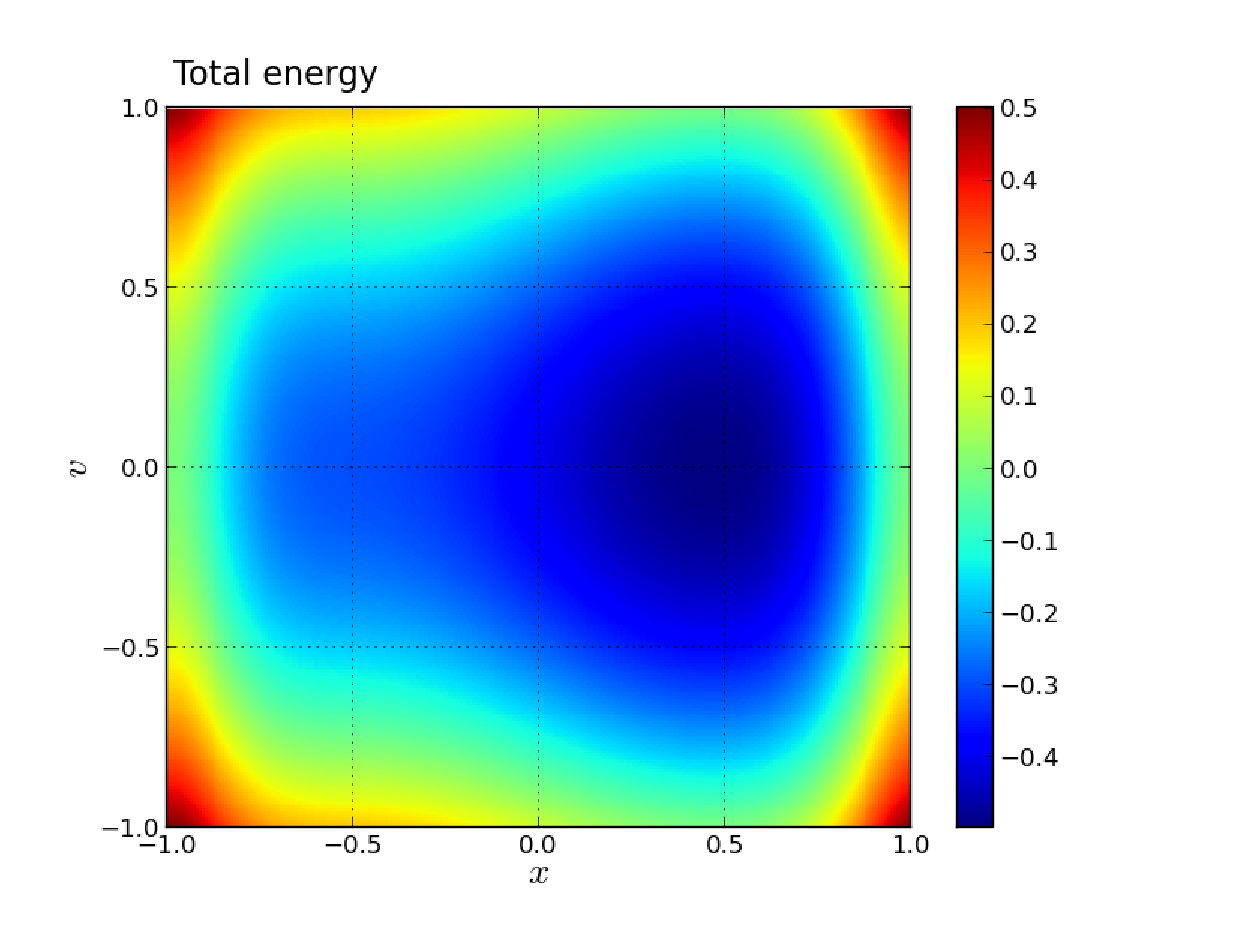
\includegraphics[scale = 0.30]{graphics/W_tot}
\end{columns}

\end{frame}

%----------------------------------------------------------------------------------------------------%
%----------------------------------------------------------------------------------------------------%

\begin{frame}{1D-1V Vlasov equation: prescribed $\vec{E}$-field, snapshots}

\vspace*{-5.5mm}
\begin{columns}
  \column{0.5\textwidth}
\begin{figure}
\centering
 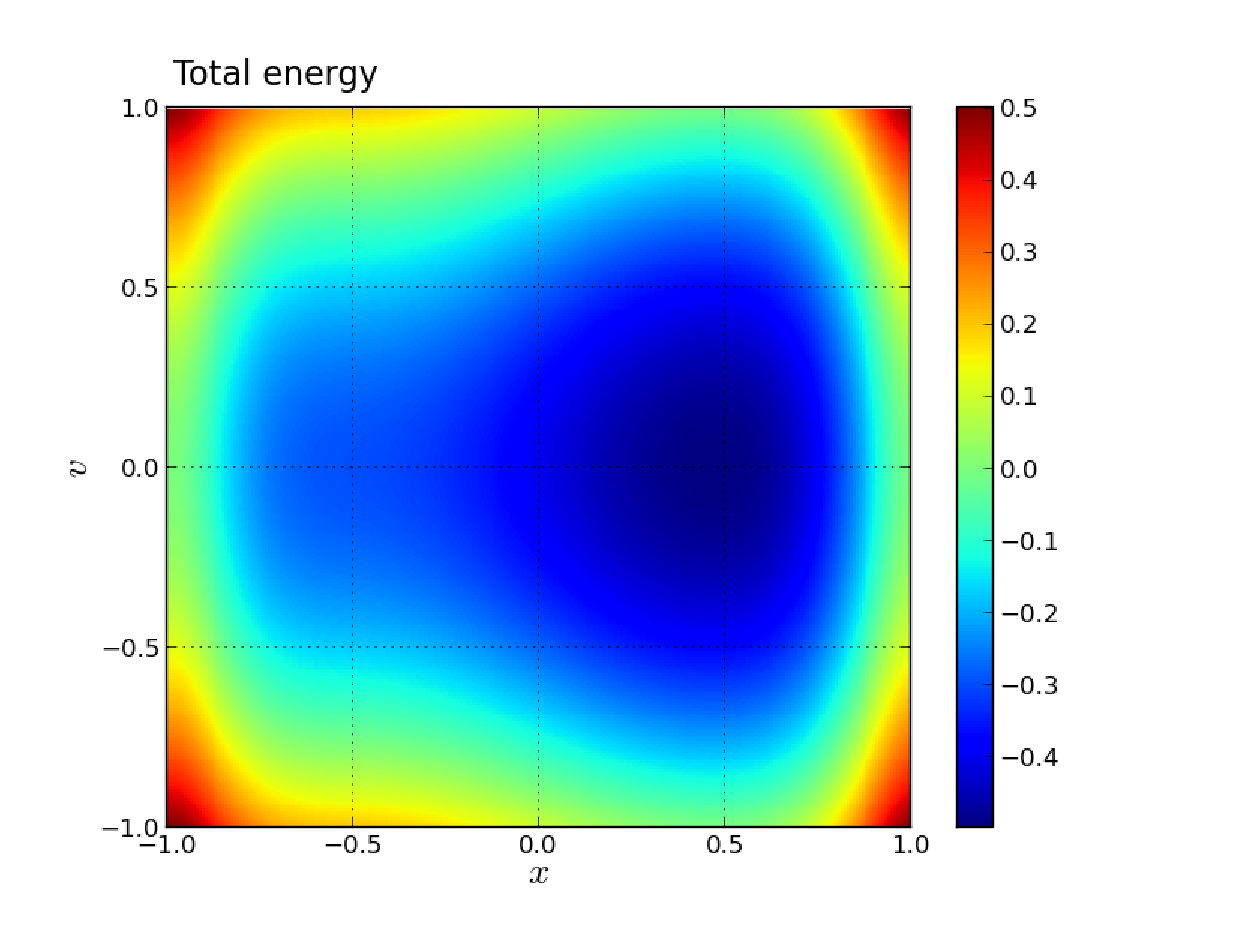
\includegraphics[width=\textwidth]{graphics/W_tot}\\ \vspace*{-4mm}
 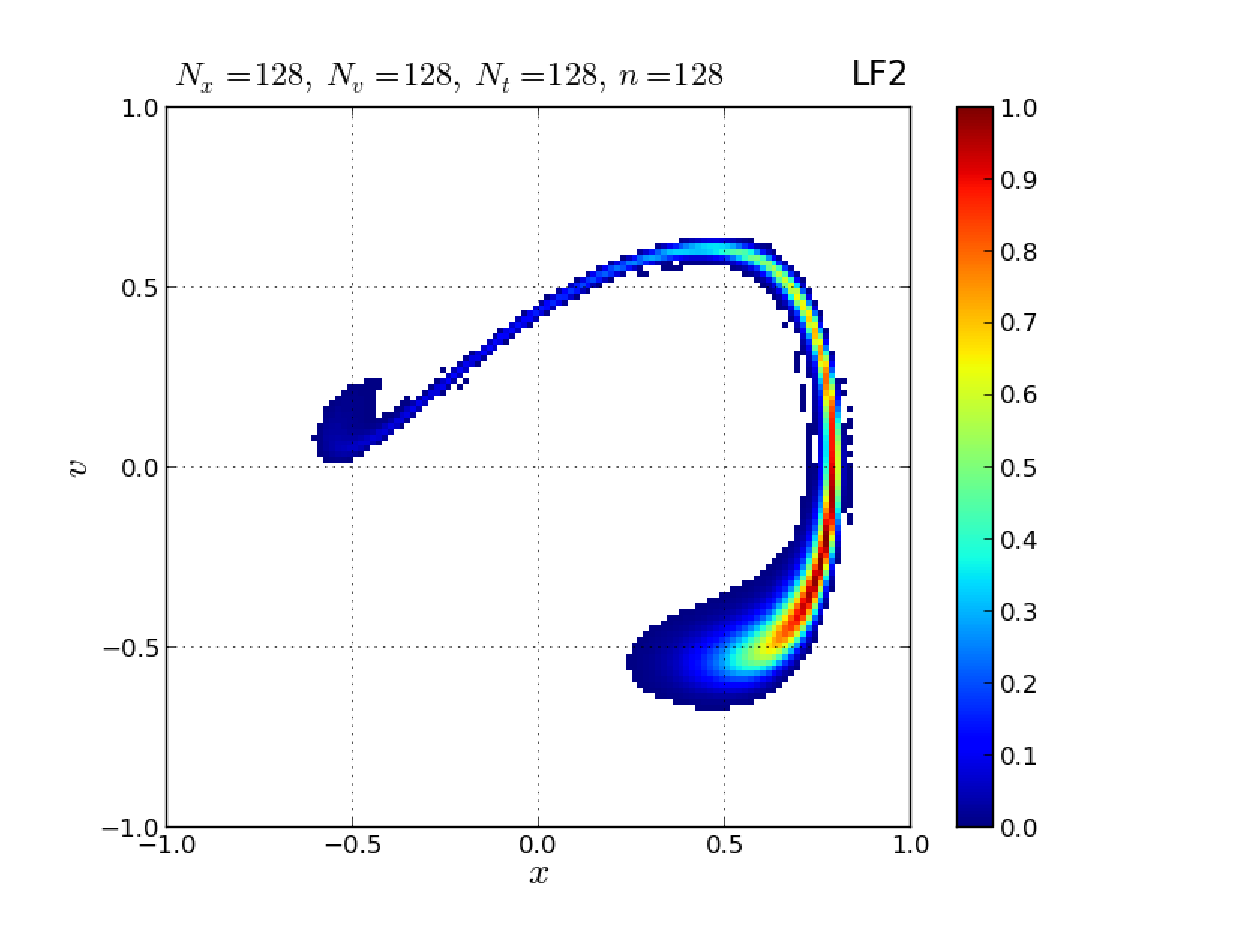
\includegraphics[width=\textwidth]{graphics/plot_-_1DVP_F12_Nx128Nv128Nt128_it00128}
\end{figure}
  \column{0.5\textwidth}
\begin{figure}
\centering
 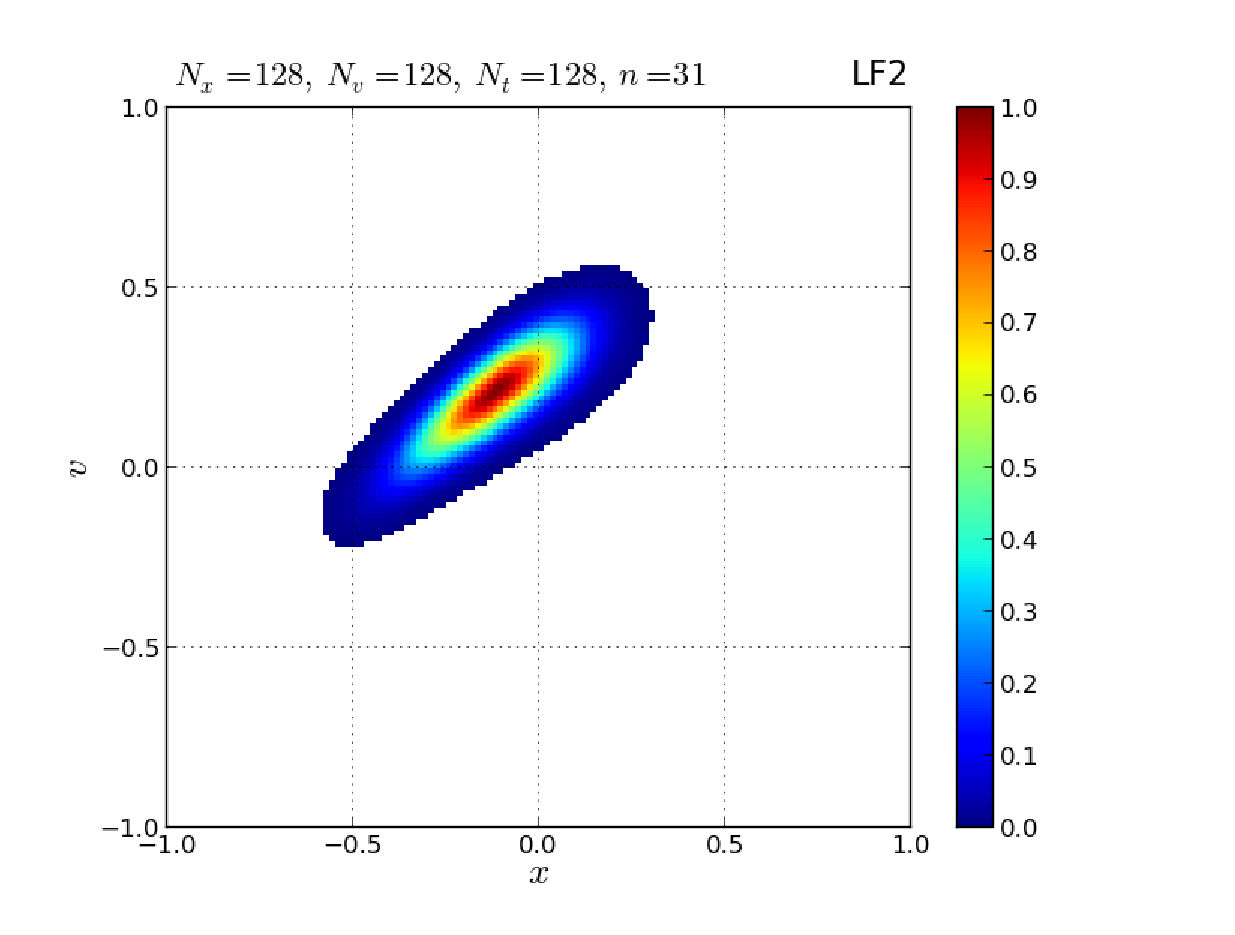
\includegraphics[width=\textwidth]{graphics/plot_-_1DVP_F12_Nx128Nv128Nt128_it00031}\\ \vspace*{-4mm}
 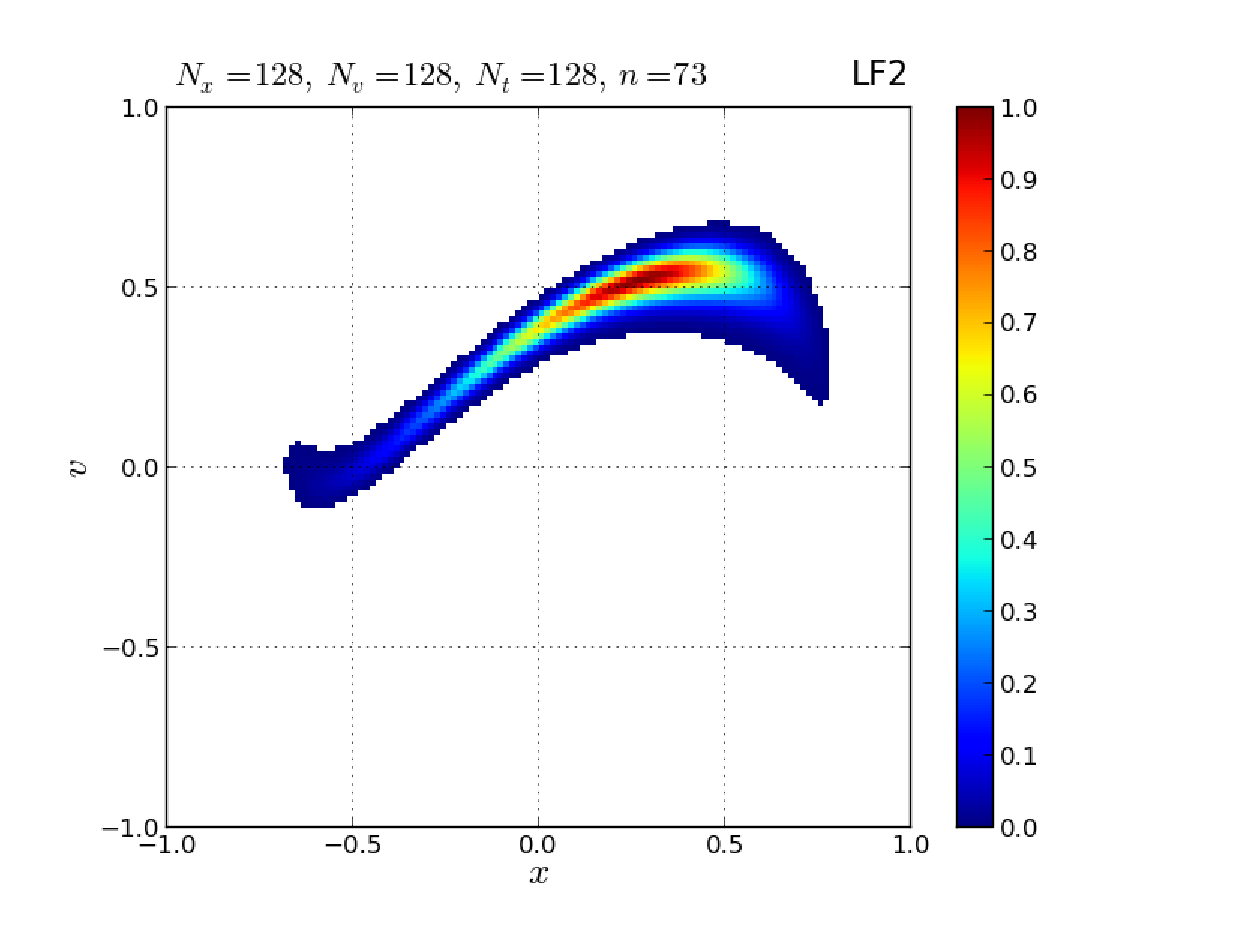
\includegraphics[width=\textwidth]{graphics/plot_-_1DVP_F12_Nx128Nv128Nt128_it00073}
\end{figure}
 \end{columns}


\end{frame}

%----------------------------------------------------------------------------------------------------%
%----------------------------------------------------------------------------------------------------%

\begin{frame}{1D-1V Vlasov equation: prescribed $\vec{E}$-field: demonstration}

\centering [show movie: plot\_-\_1DVP\_F12\_Nx256Nv256Nt256.mpeg]

\end{frame}

%----------------------------------------------------------------------------------------------------%
%----------------------------------------------------------------------------------------------------%

\section{Proposed work}
 
%----------------------------------------------------------------------------------------------------%
%----------------------------------------------------------------------------------------------------% 

\begin{frame}

\centering{\LARGE{Proposed work}}

\end{frame}

%----------------------------------------------------------------------------------------------------%
%----------------------------------------------------------------------------------------------------%

\begin{frame}{1D-1V Vlasov-Poisson system}
\begin{itemize}
\item We aim to extend the code to calculate electric field self-consistently
$$\partial_t f + v\partial_x f = 0, \qquad  \epsilon_0\partial_x^2\phi = -q \int dv f(t,x,v)$$
\item Will benchmark with bump-on-tail instability and Landau damping test cases as obtained by:
\begin{itemize}
\item \textbf{Discontinuous Galerkin:} Rossmanith, J. A. and Seal, D.C. \emph{A positivity-preserving high-order semi-Lagrangian discontinuous Galrkin scheme for the Vlasov-Poisson equations}. J. Comput. Phys. \textbf{230}, 16 (2011), p.6203--6232 
\item \textbf{Finite difference:} T. Zhou, Y. Guo., et al. \emph{Numerical study on Landau damping}. Phys. D Nonlinear Phenom. \textbf{157} (2001) p.322-333.
     \item \textbf{Convected scheme:} G\"{u}\c{c}lu, Y., et al. \emph{Arbitrarily high order convected scheme solution of the Vlasov-Poisson system}. J. Comput. Phys. \textbf{270}, 0 (2014), p.711-752.
\end{itemize}
\end{itemize}
\end{frame}
   
%----------------------------------------------------------------------------------------------------%
%----------------------------------------------------------------------------------------------------%

\begin{frame}{Boundaries}
Boundary region ($\sim$ mm thick) modeling challenges:

\begin{itemize}
    \item sharp gradients in parameters ($n$, $T$, $\phi$)
    \item vast scales and sparsity in phase space
    \item discontinuity at wall
\end{itemize}

We plan to seek high order solutions as a two-step procedure:
\begin{enumerate}
    \item local mesh refinment near wall (\emph{multiple scales of resolution}) $\Rightarrow$ will require extending high order CS to nonuniform meshes
    \item Employ an artificial compression method (ACM, or \emph{Harten}) filter to sharpen the above solution to simulate the cutoff\footnote{Harten, A. \emph{The artificial compression method for computation of shocks and contact discontinuities: III. Self-adjusting hybrid schemes} Mathematics of Computation \textbf{32}, 142 (1978), p.363--389}
\end{enumerate} 

\end{frame}

%----------------------------------------------------------------------------------------------------%
%----------------------------------------------------------------------------------------------------%

\begin{frame}{Collisions}

The chosen collision operator $\left(\frac{\partial f_{\alpha}}{\partial t}\right)_{coll} \equiv C_{\alpha\beta}(f_{\alpha},f_{\beta})$ presents variable complexity
    \begin{itemize}   
    \item \emph{Bhatnagar-Gross-Krook (BGK)} operator:
$$C_{\alpha\alpha}^{BGK} (f_{\alpha}) = \nu^{\alpha / \alpha} (v_{\alpha}) (f_{\alpha} - f_{\alpha}^{Maxwellian})$$
    \end{itemize} 
Many realistic scenarios require integral representations:
    \begin{itemize}
    \item Lorentz collision operator ($m_{\beta} \gg m_{\alpha}$)
    \item Fokker-Planck collisions \,\,\,($\Delta\theta \ll 1$)
    \item Boltzmann collision integral
    \item Landau collision operator $C_{\alpha\beta}^L$
 $$C_{\alpha\beta}^L = \frac{\partial}{\partial\vec{v}_{\alpha}}\cdot \int_{\mathbb{R}^N} d\vec{v}_{\beta}a(\vec{v}_{\alpha} - \vec{v}_{\beta})[f_{\beta}\frac{\partial f_{\alpha}}{\partial \vec{v}_{\alpha}}- f_{\alpha}\frac{\partial f_{\beta}}{\partial \vec{v}_{\beta}}]$$ 
    \item need a high order and efficient means of calculating based on high order solutions from coarser meshes $\Rightarrow$ \textbf{integral deferred correction} (IDC) by correction loops.

\end{itemize}

\end{frame}

% Fokker-Planck equation premised on particle energy changes in collision events are small (i.e. small angle approx invoked), and that the process is Markovian (i.e. f(t+dt,x) = \int f(t, x - \xi)\zeta(\xi, x - \xi )d\xi , f(t+dt) only depends on t, not before, limited memory property
  

%----------------------------------------------------------------------------------------------------%
%----------------------------------------------------------------------------------------------------%

\begin{frame}{Collisions, cont'd}
\textbf{\emph{Integral deferred correction (IDC)}} \footnote{Christlieb, A., et al. \emph{Integral deferred correction methods constructed with high-order Runge-Kutta integrators}. Mathematics of Computation (March 2009).} methods will be investigated as a predictor-corrector strategy to include high order accurate solutions with collisions\\[0.5em]

Each time step is partitioned into $m$ substeps:

$$[t^n,t^{n+1}] \quad \Rightarrow \quad t^{n} = t^{n,0} < \ldots < t^{n,m-1}= t^{n+1}$$

and loop through the following procedure for $k = 0, 1, \ldots , m-1$ for the provisional solution $f(t^{n,k})$ \footnote{arXiv:1310.6015v2}:

\begin{enumerate}
    \item Estimate the error according to IDC
    \item Evolve the error equation for $\delta^k \mapsto \delta^{k+1}$ 
    \item Correct the solution $f(t^{n,k+1}) = f(t^{n,k}) + \delta^{k+1}$ 
\end{enumerate}

\end{frame}

%----------------------------------------------------------------------------------------------------%
%----------------------------------------------------------------------------------------------------%

\begin{frame}{Collisions, cont'd}
We will apprehend collisions through the following models
\begin{itemize}
    \item BGK operator ($\alpha,\beta = e,i,n$): $C_{\alpha\alpha}^{BGK} (f_{\alpha})$\footnote{Manheimer, Wallace. et al. \emph{The development of a Krook model for nonlocal transport in laser produced plasmas}. Physics of Plasmas \textbf{15}, 083103 (2008)}
    \item Boltzmann collision integral: $C_{\alpha\beta}^B(f_{\alpha},f_{\beta},\Omega )$:
$$C_{\alpha\beta}^B = \int_{\mathbb{R}^N} dv_{\beta}\int_{S^{N-1}}d\Omega [f(v_{\alpha}')f(v_{\beta}') - f(v_{\alpha})f(v_{\beta})]K(|v_{\alpha} - v_{\beta}|, \Omega )$$

where $f : \mathbb{R}^N \mapsto \mathbb{R}_+$. This will be relevent for the case of charged particle - neutral interactions
     \item Weak form of a Landau collision operator $C_{\alpha\beta}^L$ \footnote{Gamba, Irene. et al. \emph{A conservative spectral method ofr the Boltzmann equation with anisotropic scattering and the grazing collisions limit},  arXiv:1306.4625}
\end{itemize}
We will investigate IDC and determine means for improvement

\end{frame}

%----------------------------------------------------------------------------------------------------%
%----------------------------------------------------------------------------------------------------%

\begin{frame}{Electrostatic sheath physics}

Upon completion of the above goals, we aim to simulate two charge species to explore \textbf{\emph{electrostatic sheath physics}}.

\begin{itemize}
\item Bohm sheath theory applicable for collisional plasma
\item Boundary work \,\,\,\,\quad\qquad$\Rightarrow$ can model \emph{sheath} 
\item Accurate collisions \,\quad\quad $\Rightarrow$ can model \emph{presheath}
\item kinetic solutions with self-consistent field calculations $\Rightarrow$ \emph{sheath edge} (se) kinetic Bohm criterion can be checked on ion density function $f^i$
$$\int_0^{\infty} \frac{f_{se}^i(v) dv}{v^2} \leq \frac{m_i}{kT_e}$$
\end{itemize}

Alternatively, our kinetic solutions will allow the above Bohm criterion to be used as a boundary condition so that simulations of only the edge are possible.

\end{frame}



%----------------------------------------------------------------------------------------------------%
%----------------------------------------------------------------------------------------------------%

\begin{frame}{Higher dimensions}
If possible, higher dimensions will be pursued\\[1em]
\begin{enumerate}
\item an additional velocity dimension $\Rightarrow$ magnetic fields and collisions can be included \\[1em]
\item an additional spatial dimension \,\,\,$\Rightarrow$ analysis of electrostatic effects in the edge and cross-field $B$ transport\\[1em]
\end{enumerate}

The above lends itself towards analyzing 2D edge problems and scrape-off layer transport.

\end{frame}

%----------------------------------------------------------------------------------------------------%
%----------------------------------------------------------------------------------------------------%
  


 

%We aim to continue our work and address more detailed physics. In terms of equations, the following stepthrough will be followed:
%\begin{enumerate}
%\item \textbf{advection equations}: $\partial_t f + v\partial_x f = 0$ (present work)
%\item Vlasov-Poisson system:
%$$\partial_t f + v\partial_x f + \frac{qE(x)}{m}\partial_v f = 0, \qquad \partial_x E(t,x) = \frac{q}{\epsilon_0}\int f(t,x,v)dv$$
%\item Boltzmann-Poisson system
%$$\partial_t f + v\partial_x f + \frac{qE(x)}{m}\partial_v f = (\partial_t f)_{coll}, \quad \partial_x E(t,x) = \frac{q}{\epsilon_0}\int f(t,x,v)dv$$
%\end{enumerate}



\section{Conclusions}

%----------------------------------------------------------------------------------------------------%
%----------------------------------------------------------------------------------------------------% 

\begin{frame}

\centering{\LARGE{Summary and conclusions}}

\end{frame}

%----------------------------------------------------------------------------------------------------%
%----------------------------------------------------------------------------------------------------%

\begin{frame}{Conclusions}
Motivations: 
    \begin{itemize}
    \item \fbox{\textbf{Goal}}: simulating electrostatic plasma systems
    \item \underline{\emph{Eulerian} schemes}: CFL time restriction, high resolution mesh, large memory requirements
    \item \underline{\emph{Lagrangian} schemes}: no CFL restriction, propagator for a given problem required, phase space cells filament
    \item \underline{\emph{Semi-Lagrangian} (SL) schemes}: no CFL restriction, convect phase space fluid along known particle characteristics
    \end{itemize}
\textbf{The convected scheme} (CS) is selected among SL methods:
    \begin{itemize}
    \item simple to implement (cf. discontinuous Galerkin) 
    \item advection equation solutions can be made high order 
    \item split operator methods disassemble higher dimensional equations into 1D advection equations in phase space $\Rightarrow$ can use foundation of CS solvers for higher dimensions
    \end{itemize}

\end{frame}

%----------------------------------------------------------------------------------------------------%
%----------------------------------------------------------------------------------------------------%
\begin{frame}{Conclusions, cont'd}
Summary:
    \begin{itemize} 
    \item Two varieties of CS have been implemented, distinguished by how corrections (derivatives) are computed:
        \begin{itemize}
        \item \underline{$FDN$ methods} -- by finite differences ($FD5$ shown)\\[0.5em]
        \item \underline{$FN\phantom{D}$ methods} -- calculated in Fourier space ($F2-F21$ shown)
        \end{itemize}
        \item 1D solvers applied to advection eqs.: $v$ = const and $v = v(x)$
        \item Time splitting algorithms were implemented:
        \begin{itemize} 
        \item LF2\phantom{12} -- 2nd order, 1 stage
        \item Y4\phantom{1-2}\,  -- 4th order, 3 stages
        \item O6-4\phantom{1} -- 6th order, optimized, 6 stages
        \item O11-6 -- 6th order, optimized, 11 stages
        \end{itemize}
    \item These methods were demonstrated with test cases: 
        \begin{itemize} 
        \item 2D rotating advection equation
        \item 1D-1V Vlasov equation with prescribed $\vec{E}$-field
        \end{itemize}
    \end{itemize} 
\end{frame} 

%----------------------------------------------------------------------------------------------------%
%----------------------------------------------------------------------------------------------------%

\begin{frame}{Conclusions and summary, cont'd}
Conclusions and research proposals: 
    \begin{itemize}
    \item Extend code to handle \textbf{1D-1V Vlasov-Poisson system} with self-consistent field calculations
    \item Inclusion of boundary $\Rightarrow$ \textbf{Harten filter}
    \item Inclusion of collisions $\Rightarrow$ \textbf{Deferred correction methods}
    \item With the above goals achieved $\Rightarrow$ can simulate sheath physics
    \item If progress permits, we will work towards increasing the dimensions:
        \begin{itemize}
        \item additional velocity dimension (1D-2V)  $\Rightarrow$ can include collisions and magnetic fields $\Rightarrow$ \textbf{Boltzmann-Maxwell} system
        \item additional space dimension (2D-2V) $\Rightarrow$ analysis of cross-field interplay with edge transport $\Rightarrow$ \textbf{scrape-off layer transport},
 magnetic field $\Rightarrow$ Bohm-Chodura criterion and \textbf{magnetic presheath} can be explored
        \end{itemize}
    \end{itemize}
 \end{frame} 
  
%----------------------------------------------------------------------------------------------------%
%----------------------------------------------------------------------------------------------------%



\subsection*{Thanks!}

\begin{frame}{\subsecname}
\centering    \Huge{Thank you!}
\end{frame}


\end{document}


%----------------------------------------------------------------------------------------------------%

\begin{frame}{Insert title}
Insert text
\end{frame}

%----------------------------------------------------------------------------------------------------%




